%**************************************%
%*    Generated from PreTeXt source   *%
%*    on 2018-07-24T15:26:34-04:00    *%
%*                                    *%
%*   http://mathbook.pugetsound.edu   *%
%*                                    *%
%**************************************%
\documentclass[10pt,]{book}
%% Custom Preamble Entries, early (use latex.preamble.early)
%% Default LaTeX packages
%%   1.  always employed (or nearly so) for some purpose, or
%%   2.  a stylewriter may assume their presence
\usepackage{geometry}
%% Some aspects of the preamble are conditional,
%% the LaTeX engine is one such determinant
\usepackage{ifthen}
\usepackage{ifxetex,ifluatex}
%% Raster graphics inclusion
\usepackage{graphicx}
%% Colored boxes, and much more, though mostly styling
%% skins library provides "enhanced" skin, employing tikzpicture
%% boxes may be configured as "breakable" or "unbreakable"
%% "raster" controls grids of boxes, aka side-by-side
\usepackage{tcolorbox}
\tcbuselibrary{skins}
\tcbuselibrary{breakable}
\tcbuselibrary{raster}
%% xparse allows the construction of more robust commands,
%% this is a necessity for isolating styling and behavior
%% The tcolorbox library of the same name loads the base library
\tcbuselibrary{xparse}
%% Hyperref should be here, but likes to be loaded late
%%
%% Inline math delimiters, \(, \), need to be robust
%% 2016-01-31:  latexrelease.sty  supersedes  fixltx2e.sty
%% If  latexrelease.sty  exists, bugfix is in kernel
%% If not, bugfix is in  fixltx2e.sty
%% See:  https://tug.org/TUGboat/tb36-3/tb114ltnews22.pdf
%% and read "Fewer fragile commands" in distribution's  latexchanges.pdf
\IfFileExists{latexrelease.sty}{}{\usepackage{fixltx2e}}
%% Text height identically 9 inches, text width varies on point size
%% See Bringhurst 2.1.1 on measure for recommendations
%% 75 characters per line (count spaces, punctuation) is target
%% which is the upper limit of Bringhurst's recommendations
\geometry{letterpaper,total={340pt,9.0in}}
%% Custom Page Layout Adjustments (use latex.geometry)
\geometry{paperheight=11in, paperwidth=8.5in, top=0.75in, bottom=0.75in, left=1.5in, right=1.5in}
%% This LaTeX file may be compiled with pdflatex, xelatex, or lualatex
%% The following provides engine-specific capabilities
%% Generally, xelatex and lualatex will do better languages other than US English
%% You can pick from the conditional if you will only ever use one engine
\ifthenelse{\boolean{xetex} \or \boolean{luatex}}{%
%% begin: xelatex and lualatex-specific configuration
%% fontspec package will make Latin Modern (lmodern) the default font
\ifxetex\usepackage{xltxtra}\fi
\usepackage{fontspec}
%% realscripts is the only part of xltxtra relevant to lualatex 
\ifluatex\usepackage{realscripts}\fi
%% 
%% Extensive support for other languages
\usepackage{polyglossia}
%% Main document language is US English
\setdefaultlanguage{english}
%% Spanish
\setotherlanguage{spanish}
%% Vietnamese
\setotherlanguage{vietnamese}
%% end: xelatex and lualatex-specific configuration
}{%
%% begin: pdflatex-specific configuration
%% translate common Unicode to their LaTeX equivalents
%% Also, fontenc with T1 makes CM-Super the default font
%% (\input{ix-utf8enc.dfu} from the "inputenx" package is possible addition (broken?)
\usepackage[T1]{fontenc}
\usepackage[utf8]{inputenc}
%% end: pdflatex-specific configuration
}
%% Symbols, align environment, bracket-matrix
\usepackage{amsmath}
\usepackage{amssymb}
%% allow page breaks within display mathematics anywhere
%% level 4 is maximally permissive
%% this is exactly the opposite of AMSmath package philosophy
%% there are per-display, and per-equation options to control this
%% split, aligned, gathered, and alignedat are not affected
\allowdisplaybreaks[4]
%% allow more columns to a matrix
%% can make this even bigger by overriding with  latex.preamble.late  processing option
\setcounter{MaxMatrixCols}{30}
%%
%% Color support, xcolor package
%% Always loaded, for: add/delete text, author tools
\PassOptionsToPackage{usenames,dvipsnames,svgnames,table}{xcolor}
\usepackage{xcolor}
%%
%% Semantic Macros
%% To preserve meaning in a LaTeX file
%% Only defined here if required in this document
%% Subdivision Numbering, Chapters, Sections, Subsections, etc
%% Subdivision numbers may be turned off at some level ("depth")
%% A section *always* has depth 1, contrary to us counting from the document root
%% The latex default is 3.  If a larger number is present here, then
%% removing this command may make some cross-references ambiguous
%% The precursor variable $numbering-maxlevel is checked for consistency in the common XSL file
\setcounter{secnumdepth}{3}
%% begin: General AMS environment setup
%% Environments built with amsthm package
\usepackage{amsthm}
%% Numbering for Theorems, Conjectures, Examples, Figures, etc
%% Controlled by  numbering.theorems.level  processing parameter
%% Numbering: all theorem-like numbered consecutively
%% i.e. Corollary 4.3 follows Theorem 4.2
%% Always need some theorem environment to set base numbering scheme
%% even if document has no theorems (but has other environments)
%% Create a never-used style first, always
%% simply to provide a global counter to use, namely "cthm"
\newtheorem{cthm}{BadTheoremStringName}[section]
%% end: General AMS environment setup
%% begin: environments with italicized bodies, theorems and similar
%% Style is like a theorem, and for statements without proofs
%% Theorem-like environments in modified "plain" style
%% We manage the head, do not adjust vertical spacing
%% Thus "space after theorem head" is necessary
%% This provides an automatic period after the number
\newtheoremstyle{ptxplainnotitle}
  {}% space above
  {}% space below
  {\itshape}% body font
  {}% indent amount
  {\bfseries}% theorem head font
  {.}% punctuation after theorem head
  {0.5em}% space after theorem head
  {}% theorem head specification
%% We now manage punctuation on-sight, elsewhere,
%% assuming non-trivial content inside a "title"
\newtheoremstyle{ptxplaintitle}
  {}% space above
  {}% space below
  {\itshape}% body font
  {}% indent amount
  {\bfseries}% theorem head font
  {}% punctuation after theorem head
  {0.5em}% space after theorem head
  {\thmname{#1}\thmnumber{ #2}\thmnote{ #3}}% theorem head specification
%% Only variants actually used in document appear here
%% Template eventually creates an environment of the given name
%% No arguments => Theorem 2.6. via "notitle" style variant
%% One optional argument => Theorem 2.6 Fantastic! via "title" style variant
%% AMS proof environment is basically fine as-is and special treatment
%% would certainly interfere with the functioning of \qed, etc.
%% So we simply localize the default heading
%% Redefinition of the "proof" environment is to cause a long alternate
%% title to line-break appropriately.  Code is cut verbatim, by suggestion,
%% from "Using the amsthm Package" Version 2.20.3, September 2017
%% end: environments with italicized bodies, theorems and similar
%% begin: environments with normal bodies, examples, etc.
%% Other environments go in modified "definition" style
%% Similar to above
\newtheoremstyle{ptxdefinitionnotitle}
  {}% space above
  {}% space below
  {}% body font
  {}% indent amount
  {\bfseries}% theorem head font
  {.}% punctuation after theorem head
  {0.5em}% space after theorem head
  {\thmname{#1}\thmnumber{ #2}}% theorem head specification
\newtheoremstyle{ptxdefinitiontitle}
  {}% space above
  {}% space below
  {}% body font
  {}% indent amount
  {\bfseries}% theorem head font
  {}% punctuation after theorem head
  {0.5em}% space after theorem head
  {\thmname{#1}\thmnumber{ #2}\thmnote{ #3}}% theorem head specification
\theoremstyle{ptxdefinitionnotitle}
\newtheorem{definitionnotitle}[cthm]{Definition}
\theoremstyle{ptxdefinitiontitle}
\newtheorem{definitiontitle}[cthm]{Definition}
\NewDocumentEnvironment{definition}{o}
  {\IfValueTF{#1}{\begin{definitiontitle}[#1]}{\begin{definitionnotitle}}}
  {\IfValueTF{#1}{\end{definitiontitle}}{\end{definitionnotitle}}}
\theoremstyle{ptxdefinitionnotitle}
\newtheorem{examplenotitle}[cthm]{Example}
\theoremstyle{ptxdefinitiontitle}
\newtheorem{exampletitle}[cthm]{Example}
\NewDocumentEnvironment{example}{o}
  {\IfValueTF{#1}{\begin{exampletitle}[#1]}{\begin{examplenotitle}}}
  {\IfValueTF{#1}{\end{exampletitle}}{\end{examplenotitle}}}
%% An inline exercise is like other environments
\theoremstyle{ptxdefinitionnotitle}
\newtheorem{inlineexercisenotitle}[cthm]{Checkpoint}
\theoremstyle{ptxdefinitiontitle}
\newtheorem{inlineexercisetitle}[cthm]{Checkpoint}
\NewDocumentEnvironment{inlineexercise}{o}
  {\IfValueTF{#1}{\begin{inlineexercisetitle}[#1]}{\begin{inlineexercisenotitle}}}
  {\IfValueTF{#1}{\end{inlineexercisetitle}}{\end{inlineexercisenotitle}}}
%% end: environments with normal bodies, examples, etc.
%% Divisional exercises are rendered as faux list items
%% with hard-coded numbers as arguments, not as LaTeX environments
\NewDocumentEnvironment{divisionexercise}{mo}
  {\textbf{#1}.\IfValueT{#2}{\ \textbf{#2}}\quad}
  {\par\smallskip\noindent}
%% named list environment and style
\newtcolorbox{namedlistcontent}
  {breakable, skin=enhanced, sharp corners, colback=white, colframe=black,
   boxrule=0.15ex, left skip=3ex, right skip=3ex}
%% Localize LaTeX supplied names (possibly none)
\renewcommand*{\chaptername}{Chapter}
%% Equation Numbering
%% Controlled by  numbering.equations.level  processing parameter
\numberwithin{equation}{section}
%% For improved tables
\usepackage{array}
%% Some extra height on each row is desirable, especially with horizontal rules
%% Increment determined experimentally
\setlength{\extrarowheight}{0.2ex}
%% Define variable thickness horizontal rules, full and partial
%% Thicknesses are 0.03, 0.05, 0.08 in the  booktabs  package
\makeatletter
\newcommand{\hrulethin}  {\noalign{\hrule height 0.04em}}
\newcommand{\hrulemedium}{\noalign{\hrule height 0.07em}}
\newcommand{\hrulethick} {\noalign{\hrule height 0.11em}}
%% We preserve a copy of the \setlength package before other
%% packages (extpfeil) get a chance to load packages that redefine it
\let\oldsetlength\setlength
\newlength{\Oldarrayrulewidth}
\newcommand{\crulethin}[1]%
{\noalign{\global\oldsetlength{\Oldarrayrulewidth}{\arrayrulewidth}}%
\noalign{\global\oldsetlength{\arrayrulewidth}{0.04em}}\cline{#1}%
\noalign{\global\oldsetlength{\arrayrulewidth}{\Oldarrayrulewidth}}}%
\newcommand{\crulemedium}[1]%
{\noalign{\global\oldsetlength{\Oldarrayrulewidth}{\arrayrulewidth}}%
\noalign{\global\oldsetlength{\arrayrulewidth}{0.07em}}\cline{#1}%
\noalign{\global\oldsetlength{\arrayrulewidth}{\Oldarrayrulewidth}}}
\newcommand{\crulethick}[1]%
{\noalign{\global\oldsetlength{\Oldarrayrulewidth}{\arrayrulewidth}}%
\noalign{\global\oldsetlength{\arrayrulewidth}{0.11em}}\cline{#1}%
\noalign{\global\oldsetlength{\arrayrulewidth}{\Oldarrayrulewidth}}}
%% Single letter column specifiers defined via array package
\newcolumntype{A}{!{\vrule width 0.04em}}
\newcolumntype{B}{!{\vrule width 0.07em}}
\newcolumntype{C}{!{\vrule width 0.11em}}
\makeatother
%% Figures, Tables, Listings, Named Lists, Floats
%% The [H]ere option of the float package fixes floats in-place,
%% in deference to web usage, where floats are totally irrelevant
%% You can remove some of this setup, to restore standard LaTeX behavior
%% HOWEVER, numbering of figures/tables AND theorems/examples/remarks, etc
%% may de-synchronize with the numbering in the HTML version
%% You can remove the "placement={H}" option to allow flotation and
%% preserve numbering, BUT the numbering may then appear "out-of-order"
%% Floating environments: http://tex.stackexchange.com/questions/95631/
\usepackage{float}
\usepackage{newfloat}
\usepackage{caption}%% Adjust stock figure environment so that it no longer floats
\SetupFloatingEnvironment{figure}{fileext=lof,placement={H},within=section,name=Figure}
\captionsetup[figure]{labelfont=bf}
%% http://tex.stackexchange.com/questions/16195
\makeatletter
\let\c@figure\c@cthm
\makeatother
%% Adjust stock table environment so that it no longer floats
\SetupFloatingEnvironment{table}{fileext=lot,placement={H},within=section,name=Table}
\captionsetup[table]{labelfont=bf}
%% http://tex.stackexchange.com/questions/16195
\makeatletter
\let\c@table\c@cthm
\makeatother
%% Create "named list" environment to hold lists with captions
%% We do not use a floating environment, so list can page-break
\newenvironment{namedlist}{\par\bigskip\noindent}{}
%% New caption type for numbering, style, etc.
\DeclareCaptionType[within=section]{namedlistcap}[List]
\captionsetup[namedlistcap]{labelfont=bf,aboveskip=1.0ex,belowskip=\baselineskip}
%% http://tex.stackexchange.com/questions/16195
\makeatletter
\let\c@namedlistcap\c@cthm
\makeatother
%% Footnote Numbering
%% We reset the footnote counter, as given by numbering.footnotes.level
\makeatletter\@addtoreset{footnote}{section}\makeatother
%% More flexible list management, esp. for references
%% But also for specifying labels (i.e. custom order) on nested lists
\usepackage{enumitem}
%% Indented groups of "exercise" within an "exercises" division
%% tcolorbox styles for exercisegroup layout
%% We use a LaTeX length to pass a width from the enclosing
%% exercisegroup (parameterized by the number of columns)
%% down into the environment for the actual exercises.
%% "exercise group exercise width"
\newlength{\egexwidth}
%% An "exercise group exercise" has a bold number inline at
%% the start of the exercise.  This serial number is a parameter
%% of the tcolorbox "egexercise" environment, so is passed to "title".
%% Debug: to make spacing obvious, set "colback=green" in "exgroupexstyle"
\tcbset{ exgroupexstyle/.style={size=minimal,width=\egexwidth,colback=white,frame empty,valign=top,coltitle=black,fonttitle=\bfseries,attach title to upper,after title={.\space}} }
\DeclareTColorBox{egexercise}{m}{title=#1, exgroupexstyle}
%% An "xparse" environment will represent the entire exercise group,
%% with the number of columns as a parameter.
%% TODO: make the 1-column version the default without an argument, bail on raster
%% The "egexwidth" length gets set on entry, widths are computed in XSL stylesheet
%% The overall indentation and gaps are also hard-coded in the XSL
%% The "solution" version only changes to no-indentation
\tcbset{ exgroupstyle/.style={raster equal height=rows,raster force size=false, raster left skip=0.05\linewidth, raster column skip=
0.03\linewidth} }
\tcbset{ exgroupsolutionstyle/.style={raster equal height=rows,raster force size=false, raster right skip=0.05\linewidth, raster column skip=
0.03\linewidth} }
\NewDocumentEnvironment{exercisegroup}{m}
  {\setlength{\egexwidth}{\ifx1#1{0.95}\fi\ifx2#1{0.46}\fi\ifx3#1{0.296666666666667}\fi\ifx4#1{0.215}\fi\ifx5#1{0.166}\fi\ifx6#1{0.166}\fi\linewidth}
   \begin{tcbraster}
    [exgroupstyle,raster columns=#1]}
  {\end{tcbraster}}
\NewDocumentEnvironment{exercisegroupsolution}{m}
  {\setlength{\egexwidth}{\ifx1#1{0.95}\fi\ifx2#1{0.46}\fi\ifx3#1{0.296666666666667}\fi\ifx4#1{0.215}\fi\ifx5#1{0.166}\fi\ifx6#1{0.166}\fi\linewidth}
   \begin{tcbraster}
    [exgroupsolutionstyle,raster columns=#1]}
  {\end{tcbraster}}
%% hyperref driver does not need to be specified, it will be detected
\usepackage{hyperref}
%% Hyperlinking active in PDFs, all links solid and blue
\hypersetup{colorlinks=true,linkcolor=blue,citecolor=blue,filecolor=blue,urlcolor=blue}
\hypersetup{pdftitle={Contemporary Pre-Calculus Through Applications}}
%% If you manually remove hyperref, leave in this next command
\providecommand\phantomsection{}
%% Graphics Preamble Entries
\usepackage{tikz}
\usepackage{pgfplots}
\usepackage{pgfplotstable}
\pgfplotsset{axis lines = middle,
   x label style={at={(axis description cs:0.5,0)}, anchor=north},
   y label style={at={(axis description cs:0,.5)}, rotate=90, anchor=south},
   scaled y ticks=false,
   /pgfplots/xlabel near ticks/.style={
      /pgfplots/every axis x label/.style={
        at={(ticklabel cs:0.5)},anchor=near ticklabel
        }
      },
   /pgfplots/ylabel near ticks/.style={
      /pgfplots/every axis y label/.style={
        at={(ticklabel cs:0.5)},rotate=90,anchor=near ticklabel}
        }
      }
\usetikzlibrary{backgrounds}
\usetikzlibrary{arrows,matrix}
\usetikzlibrary{snakes}
%% If tikz has been loaded, replace ampersand with \amp macro
\ifdefined\tikzset
    \tikzset{ampersand replacement = \amp}
\fi
%% tcolorbox styles for sidebyside layout
\tcbset{ sbsstyle/.style={raster equal height=rows,raster force size=false} }
\tcbset{ sbsheadingstyle/.style={size=minimal,halign=center,fontupper=\bfseries,colback=white,frame empty} }
\tcbset{ sbspanelstyle/.style={size=minimal,colback=white,frame empty} }
\tcbset{ sbscaptionstyle/.style={size=minimal,halign=center,colback=white,frame empty} }
%% Enviroments for side-by-side and components
%% Necessary to use \NewTColorBox for boxes of the panels
%% "newfloat" environment to squash page-breaks within a single sidebyside
\DeclareFloatingEnvironment[placement={H}]{sbscontainer}
%% "xparse" environment for entire sidebyside
\NewDocumentEnvironment{sidebyside}{mmmm}
  {\begin{sbscontainer}\begin{tcbraster}
    [sbsstyle,raster columns=#1,
    raster left skip=#2\linewidth,raster right skip=#3\linewidth,raster column skip=#4\linewidth]}
  {\end{tcbraster}\end{sbscontainer}}
%% "tcolorbox" environments for three components of a panel
\NewTColorBox{sbsheading}{m}{sbsheadingstyle,width=#1\linewidth}
\NewTColorBox{sbspanel}{mO{top}}{sbspanelstyle,width=#1\linewidth,valign=#2}
\NewTColorBox{sbscaption}{m}{sbscaptionstyle,width=#1\linewidth}
%% extpfeil package for certain extensible arrows,
%% as also provided by MathJax extension of the same name
%% NB: this package loads mtools, which loads calc, which redefines
%%     \setlength, so it can be removed if it seems to be in the 
%%     way and your math does not use:
%%     
%%     \xtwoheadrightarrow, \xtwoheadleftarrow, \xmapsto, \xlongequal, \xtofrom
%%     
%%     we have had to be extra careful with variable thickness
%%     lines in tables, and so also load this package late
\usepackage{extpfeil}
%% Custom Preamble Entries, late (use latex.preamble.late)
%% Begin: Author-provided packages
%% (From  docinfo/latex-preamble/package  elements)
%% End: Author-provided packages
%% Begin: Author-provided macros
%% (From  docinfo/macros  element)
%% Plus three from MBX for XML characters

\newcommand{\lt}{<}
\newcommand{\gt}{>}
\newcommand{\amp}{&}
%% End: Author-provided macros
\begin{document}
\frontmatter
%% begin: half-title
\thispagestyle{empty}
{\centering
\vspace*{0.28\textheight}
{\Huge Contemporary Pre-Calculus Through Applications}\\}
\clearpage
%% end:   half-title
%% begin: adcard
\thispagestyle{empty}
\null%
\clearpage
%% end:   adcard
%% begin: title page
%% Inspired by Peter Wilson's "titleDB" in "titlepages" CTAN package
\thispagestyle{empty}
{\centering
\vspace*{0.14\textheight}
%% Target for xref to top-level element is ToC
\addtocontents{toc}{\protect\hypertarget{cpta}{}}
{\Huge Contemporary Pre-Calculus Through Applications}\\[3\baselineskip]
{\Large Mathematics Department}\\[0.5\baselineskip]
{\Large North Carolina School of Science and Mathematics}\\[3\baselineskip]
{\Large July 24, 2018}\\}
\clearpage
%% end:   title page
%% begin: copyright-page
\thispagestyle{empty}
\vspace*{\stretch{2}}
\vspace*{\stretch{1}}
\null\clearpage
%% end:   copyright-page
%% begin: table of contents
%% Adjust Table of Contents
\setcounter{tocdepth}{1}
\renewcommand*\contentsname{Contents}
\tableofcontents
%% end:   table of contents
\mainmatter
\typeout{************************************************}
\typeout{Chapter 1 Data}
\typeout{************************************************}
\chapter[{Data}]{Data}\label{chapter01}
\hypertarget{p-1}{}%
Introduction to this chapter%
\typeout{************************************************}
\typeout{Section 1.1 }
\typeout{************************************************}
\section[{}]{}\label{chapter01-section01}
\typeout{************************************************}
\typeout{Chapter 2 Transformations of Functions}
\typeout{************************************************}
\chapter[{Transformations of Functions}]{Transformations of Functions}\label{chapter02}
\hypertarget{p-2}{}%
Introduction to this chapter%
\typeout{************************************************}
\typeout{Section 2.1 }
\typeout{************************************************}
\section[{}]{}\label{chapter02-section01}
\typeout{************************************************}
\typeout{Chapter 3 Combining Functions}
\typeout{************************************************}
\chapter[{Combining Functions}]{Combining Functions}\label{chapter03}
\hypertarget{p-3}{}%
Introduction to this chapter%
\typeout{************************************************}
\typeout{Section 3.1 }
\typeout{************************************************}
\section[{}]{}\label{chapter03-section01}
\typeout{************************************************}
\typeout{Chapter 4 Exponential Functions}
\typeout{************************************************}
\chapter[{Exponential Functions}]{Exponential Functions}\label{chapter04}
\typeout{************************************************}
\typeout{Section 4.1 Recursive Functions}
\typeout{************************************************}
\section[{Recursive Functions}]{Recursive Functions}\label{chapter04-section01}
\hypertarget{p-4}{}%
In a previous chapter we learned that a function is a special sets of ordered pairs.  In most of the examples in the preceeding chapters, functions were described by an algebraic expression that could be evaluated for a particular input value resulting in a unique output value. Such algebraic expressions are called closed form or explicit expressions.  For these functions, the relationship \(y=f(x)\) is used to show how the \(y\)-value is related to the given \(x\)-value. For example, the function \(f(x)=x^2+6x\) is an explicit function. This notation tells us that any particular numerical value for \(x\) is paired with the \(y\)-value equal to \(x^2+6x\). So 1 is paired with 7, since \(f(1)=(1)^2+6(1)=7\) , and \(-3\) is paired with \(-9\), since \(f(-3)=(-3)^2+6(-3)=-9\).%
\par
\hypertarget{p-5}{}%
In this section we will investigate functions that are defined recursively. The domain values for these functions are positive whole numbers, and each range value is defined in terms of the preceding range value, rather than in terms of an \(x\)-value.%
\begin{example}[{Ibuprofen in the blood stream.}]\label{ibuprofen-example-one-dose}
\hypertarget{p-6}{}%
Joan has a headache and decides to take a 200mg ibuprofen tablet for pain relief.  The drug is absorbed into her system and stays in her system until the drug is metabolized and filtered out by the liver and kidneys.  Ibuprofen is rapidly metabolized.  Every four hours, Joan's body removes \(67\%\) of the ibuprofen that was in her body at the beginning of that four-hour time period.  How much of the ibuprofen will remain in her system \(24\) hours after taking the \(200\)mg tablet?%
\par\smallskip%
\noindent\textbf{Solution}.\hypertarget{solution-1}{}\quad%
\hypertarget{p-7}{}%
One way to generate values for the amount of ibuprofen in Joan's system is to use an iterative process.  In any iterative process the current value of a variable is used to determine the next value.  In this example, we generate a new amount of ibuprofen by subtracting the amount of ibuprofen filtered out of Joan's system from the amount that was previously there.  Since Joan begins with 200mg of ibuprofen, we write%
\begin{gather*}
D_0 = 200
\end{gather*}
where \(D_0\) is used to represent the amount of ibuprofen present at the start of the process%
\par
\hypertarget{p-8}{}%
We will use \(D_1\) to represent the amount of ibuprofen left after four hours.  The subscripts are used to count the steps, or iterations,  in the iterative process. In this problem the subscript  represents the number of four-hour time periods since Joan took the tablet.  In four hours, her kidneys have filtered out \(67\%\) of the drug from her bloodstream, so we write%
\begin{gather*}
D_1=D_0-.67D_0=200-.67 \cdot 200 = 66
\end{gather*}
%
\par
\hypertarget{p-9}{}%
The amount of drug in her body after a second four-hour time period is represented by \(D_2\).%
\begin{gather*}
D_2=D_1-0.67D_1=66-.067 \cdot 66 = 21.78
\end{gather*}
%
\par
\hypertarget{p-10}{}%
Similarly, we know that successive values of the amount of drug in her body can be generated by%
\begin{align*}
D_3 \amp = D_2-0.67D_2 = 7.187\\
D_4 \amp = D_3-0.67D_3 = 2.372
\end{align*}
and, in general,%
\begin{gather*}
D_n=D_{n-1}-0.67D_{n-1},n=1,2,3...
\end{gather*}
%
\par
\hypertarget{p-11}{}%
Using a spreadsheet or calculator, we can generate successive values of \(D_n\) as shown in \hyperref[figure-ibuprofen-one-dose]{Figure~2}.  Note that values in the table are rounded to three decimal places but that exact values were used in all computations. The amount of drug in Joan's body drops to less than \(1\) mg between the fourth and fifth time periods.  If she takes a single \(200\) mg dose, Joan will have only about \(0.258\) mg remaining in her body \(24\) hours later.%
\begin{figure}
\centering
\begin{sidebyside}{2}{0.0375}{0.0375}{0.075}
\begin{sbspanel}{0.2}
\resizebox{\linewidth}{!}{{
\pgfplotstabletypeset[
col sep=comma,
column type=l,
every head row/.style={after row=\hline},
every column/.style={column type/.add={|}{|}},
every first column/.style={column type/.add={}{|}},
columns/0/.style={string type, column name={$n$}},
columns/1/.style={string type, column name={$D_n$}},
]{data-single-dose-ibuprofen.csv}
}
}
\end{sbspanel}
\begin{sbspanel}{0.65}
\resizebox{\linewidth}{!}{{
\begin{tikzpicture}
\begin{axis}[
axis line style = {<->},
width = 0.5\linewidth,
xlabel = Number of 4 hour intervals,
ylabel = Amount of Ibuprofen (mg),
label style={font=\tiny},
xmin = -1, xmax= 7,
ymin = -25, ymax=250,
ytick = {0,100,200},
xtick = {0, 1, ...,6},
tick label style={font=\tiny},
]
\addplot table [only marks, x index = {0}, y index = {1}, col sep=comma]{data-single-dose-ibuprofen.csv};
\end{axis}
\end{tikzpicture}
}
}
\end{sbspanel}
\end{sidebyside}
\caption{Amount of drug in Joan's body (Single 200 mg dose)\label{figure-ibuprofen-one-dose}}
\end{figure}
\hypertarget{p-12}{}%
The graph in \hyperref[figure-ibuprofen-one-dose]{Figure~2} shows the ordered pairs \((n,D_n)\) generated by the recursive system%
%
\begin{gather*}
D_0=200\\
D_n=D_{n-1} - 0.67D_{n-1}, n=1,2,3,...
\end{gather*}
\hypertarget{p-13}{}%
Each point on the graph shows the amount of ibuprofen in Joan’s body at the end of a four-hour time period. Notice that there is obvious curvature in this graph.  The amount of drug in Joan’s body does not decrease by the same number of milligrams during each time interval.%
\end{example}
\typeout{************************************************}
\typeout{Exercises 4.1.1 Class Practice}
\typeout{************************************************}
\subsection[{Class Practice}]{Class Practice}\label{exercises-1}
\begin{divisionexercise}{1}\hypertarget{chapter04-section01-initial-ibuprofen-exercise}{}
\hypertarget{p-14}{}%
Modify the recursive system used in \hyperref[ibuprofen-example-one-dose]{Example~1} as appropriate to answer the following questions: \leavevmode%
\begin{enumerate}[label=(\alph*)]
\item\hypertarget{li-1}{}Suppose Joan takes tablets that contain \(250\) milligrams of ibuprofen. How much ibuprofen would be in her body after \(4, 8, 12, 16, 20,\) and \(24\) hours?%
\item\hypertarget{li-2}{}Suppose Joan's kidneys filter only \(50\%\) of the drug in a four hour time period.  If Joan takes a \(200\) mg tablet every \(4\) hours, how much ibuprofen would she have in her system after \(4, 8, 12, 16, 20,\) and \(24\) hours?%
\end{enumerate}
%
\end{divisionexercise}%
\begin{divisionexercise}{2}\hypertarget{exercise-2}{}
\hypertarget{p-15}{}%
In each recursive system, the domain of \(D_n\) is \(n=1,2,3, ...\) and \(D_n\) represents the amount of ibuprofen in Joan's system after n four-hour time periods.  For each system, find how much drug remains after \(24\) hours, and identify the rate at which Joan's system filters out the drug. \leavevmode%
\begin{enumerate}[label=(\alph*)]
\item\hypertarget{li-3}{}\(D_0=300, D_n=D_{n-1} - 0.8D_{n-1}\)%
\item\hypertarget{li-4}{}\(D_0=150, D_n=D_{n-1} - 0.2D_{n-1}\)%
\item\hypertarget{li-5}{}\(D_0=500, D_n=0.2D_{n-1}\)%
\item\hypertarget{li-6}{}\(D_0=500, D_n=0.5D_{n-1}\)%
\end{enumerate}
%
\end{divisionexercise}%
\begin{example}[{Repated dose of ibuprofen.}]\label{example-2}
\hypertarget{p-16}{}%
Joan strained her knee playing tennis and her doctor has prescribed ibuprofen to reduce the inflammation and control pain.  Joan is instructed to take two 200-milligram ibuprofen tablets every 4 hours for three days.  Joan doesn’t like taking medicine, so she decides to take only one tablet every four hours for six days.  After the six days, Joan’s knee has not responded to the medication.  Naturally, she knew that the knee would take longer to respond to the reduced treatment, but she did not expect no response at all.  What could have happened?%
\par\smallskip%
\noindent\textbf{Solution}.\hypertarget{solution-2}{}\quad%
\hypertarget{p-17}{}%
In this situation, Joan did not take just a single 200 mg tablet.  Every four hours she took another 200 mg tablet, and we can modify our recursive system to model this behavior. At the end of the nth four-hour period, Joan’s body has filtered \(67\%\) of the drug that was in her body after n-1st  four-hour period.  In addition, 200 mg from the new tablet have been added into her body.  The recursive system representing the amount of ibuprofen in Joan’s body if she takes one tablet every four hours is%
%
\begin{gather*}
D_0=200\\
D_n=D_{n-1} - 0.67D_{n-1} + 200, n=1,2,3,...
\end{gather*}
\hypertarget{p-18}{}%
The subscript n represents the number of four-hour time periods that have elapsed since Joan took the first dose.  By iterating the recursive system we can generate values of \(D_n\) that represent the amounts of drug in Joan’s body at the end of each four-hour period, assuming  \(67\%\) of the drug is filtered in a four-hour period.  These values, rounded to two decimal places, are shown together with a graph in \hyperref[figure-ibuprofen-multi-dose]{Figure~4}%
\begin{figure}
\centering
\begin{sidebyside}{2}{0.0375}{0.0375}{0.075}
\begin{sbspanel}{0.2}
\resizebox{\linewidth}{!}{{
\pgfplotstabletypeset[
col sep=comma,
column type=l,
every head row/.style={after row=\hline},
every column/.style={column type/.add={|}{|}},
every first column/.style={column type/.add={}{|}},
columns/0/.style={string type, column name={$n$}},
columns/1/.style={string type, column name={$D_n$}},
]{data-multi-dose-ibuprofen.csv}
}
}
\end{sbspanel}
\begin{sbspanel}{0.65}
\resizebox{\linewidth}{!}{{
\begin{tikzpicture}
\begin{axis}[
axis line style = {<->},
width = 0.5\linewidth,
xlabel = Number of 4 hour intervals,
ylabel = Amount of Ibuprofen (mg),
label style={font=\tiny},
xmin = -1.5, xmax= 11,
ymin = -30, ymax=350,
ytick = {0,100,200,300},
xtick = {0, 1, ...,10},
tick label style={font=\tiny},
]
\addplot table [only marks, x index = {0}, y index = {1}, col sep=comma]{data-multi-dose-ibuprofen.csv};
\end{axis}
\end{tikzpicture}
}
}
\end{sbspanel}
\end{sidebyside}
\caption{Amount of drug in Joan's body (Reoccuring 200 mg doses)\label{figure-ibuprofen-multi-dose}}
\end{figure}
\hypertarget{p-19}{}%
The points shown in \hyperref[figure-ibuprofen-multi-dose]{Figure~4} represent the amount of the drug in Joan’s body immediately after she takes a tablet.  Between consecutrive doses, we know that the level of the drug declines.  We assume that the level “jumps up” at the moment she takes another tablet, and the recursive system enables us to compute these values.   If we  record the drug levels only after she takes a tablet, then we see that these values reach an equilibrium of approximately 298.51 mg.  To see why this equilibrium has been reached, consider how much of the 298.51 mg of the drug will be filtered in four hours.  Joan’s kidneys will filter out \(67\%\) of the 298.51 mg in her body, or approximately 200 mg, which will be replaced when she takes the next tablet. Equilibrium occurs because the amount of drug taken into the body is the same as the amount filtered prior to taking the next tablet.%
\par
\hypertarget{p-20}{}%
Suppose the drug Joan is taking has a therapeutic level of 450 mg.  This means that there must be at least 450 milligrams of the drug in her body for Joan to receive the benefits of the drug.  No wonder she thought the drug was not working.  It wasn’t!%
\end{example}
\typeout{************************************************}
\typeout{Exercises 4.1.2 Exercises}
\typeout{************************************************}
\subsection[{Exercises}]{Exercises}\label{exercises-2}
\begin{divisionexercise}{1}\hypertarget{exercise-3}{}
\hypertarget{p-21}{}%
Modify the recursive  system  used in \hyperref[ibuprofen-example-one-dose]{Example~1} as appropriate to answer the following questions: \leavevmode%
\begin{enumerate}[label=(\alph*)]
\item\hypertarget{li-7}{}Suppose Joan takes tablets that contain 250 milligrams of ibuprofen.  How much ibuprofen would be in her body after 4, 8, 12, 16, 20, and 24 hours?%
\item\hypertarget{li-8}{}Suppose Joan’s kidneys filter only \(50\%\) of the drug in a four hour time period.  If Joan takes a 200 mg tablet every 4 hours, how much ibuprofen would she  have in her system after  4, 8, 12, 16, 20 and 24 hours?%
\end{enumerate}
%
\end{divisionexercise}%
\begin{divisionexercise}{2}\hypertarget{exercise-4}{}
\hypertarget{p-22}{}%
If Joan takes her medication every 4 hours, determine the amount of drug in Joan’s body after 2 days (twelve  4-hour time periods) and the equilibrium level resulting from each of the following recursive systems.  Plot the ordered pairs you generate on a graph.  Note that in some cases the initial dosage and subsequent doses are not the same size.  In each exercise, the domain of \(D_n\) is \(n=1,2,3, ...\) \leavevmode%
\begin{enumerate}[label=(\alph*)]
\item\hypertarget{li-9}{}\(D_0=200, D_n=D_{n-1} - 0.4D_{n-1} + 200\)%
\item\hypertarget{li-10}{}\(D_0=800, D_n=0.6D_{n-1} + 200\)%
\item\hypertarget{li-11}{}\(D_0=600, D_n=0.4D_{n-1} + 200\)%
\item\hypertarget{li-12}{}\(D_0=600, D_n=D_{n-1} - 0.4D_{n-1} + 200\)%
\item\hypertarget{li-13}{}\(D_0=600, D_n=0.6D_{n-1} + 300\)%
\item\hypertarget{li-14}{}\(D_0=600, D_n=0.4D_{n-1} + 300\)%
\end{enumerate}
%
\end{divisionexercise}%
\begin{divisionexercise}{3}\hypertarget{exercise-5}{}
\hypertarget{p-23}{}%
Each of the systems in exercise 2 can be written in the form%
\begin{gather*}
D_0=a\\
D_n=(1-r) D_{n-1}+b, n=1,2,3...
\end{gather*}
\leavevmode%
\begin{enumerate}[label=(\alph*)]
\item\hypertarget{li-15}{}What does \(r\) represent in the context of Joan's medication?  Why is \(r\) between 0 and 1?%
\item\hypertarget{li-16}{}By looking back at the results of exercise 2 and by trying other variations, determine the effect of changing \(a\), \(r\), and \(b\) on the amount of drug in Joan's body after 5 days.%
\item\hypertarget{li-17}{}Determine the equilibrium level in terms of \(a\), \(r\), and \(b\).  You can recognize that equilibrium has been reached if  \(D_n=D_{n-1}\).%
\item\hypertarget{li-18}{}Use the result of part c to determine the equilibrium level of a drug if you take 200 mg every 4 hours and your kidneys filter out \(50\%\) of the drug in your body every 4 hours.%
\end{enumerate}
%
\end{divisionexercise}%
\begin{divisionexercise}{4}\hypertarget{exercise-6}{}
\hypertarget{p-24}{}%
A company has \(\$10,000\) worth of equipment and for tax purposes they want to figure the depreciation of the equipment over a 10-year time period.  One method is to reduce the value each year by the same dollar amount.  A second method is to decrease the value of the equipment each year by the same percent of the current value each year. \leavevmode%
\begin{enumerate}[label=(\alph*)]
\item\hypertarget{li-19}{}Using the first method, generate a table and graph for the value of the equipment if it is  decreased each year by \(\$2000\).%
\item\hypertarget{li-20}{}Using the second method, generate a table and graph for the value of the equipment if it is decreased by \(20\%\) each year.%
\end{enumerate}
%
\end{divisionexercise}%
\begin{divisionexercise}{5}\hypertarget{exercise-7}{}
\hypertarget{p-25}{}%
One of the primary responsibilities of the manager of a swimming pool is to maintain the proper concentration of chlorine in the swimming pool.  The concentration should be between 1 and 2 parts per million (ppm).  If the concentration gets as high as 3 ppm swimmers experience burning eyes.  If the concentration gets below 1 ppm, the water will become cloudy, which is unappealing.  If it drops below 0.5 ppm, algae begin to grow.  During a period of one day, \(15\%\) of the chlorine present in the pool dissipates (mainly due to the sun). \leavevmode%
\begin{enumerate}[label=(\alph*)]
\item\hypertarget{li-21}{}If the chlorine content starts at 2.5 ppm and no additional chlorine is added, how long will it be before the water becomes cloudy?%
\item\hypertarget{li-22}{}If the chlorine content starts at 2.5 ppm and the equivalent of 0.5 ppm of chlorine is added daily, what will happen to the level of chlorine in the pool in the long run?%
\item\hypertarget{li-23}{}If the chlorine content starts at 2.5 ppm and the equivalent of 0.1 ppm of chlorine is added daily, what will happen to the level of chlorine in the pool in the long run?%
\item\hypertarget{li-24}{}How much chlorine must be added daily for the chlorine level to stabilize at 1.8 ppm?%
\end{enumerate}
%
\end{divisionexercise}%
\begin{divisionexercise}{6}\hypertarget{exercise-8}{}
\hypertarget{p-26}{}%
The Fish and Wildlife Division monitors the trout population in a stream that is under their jurisdiction.  Their research indicates that natural predators, together with pollution and fishing, are causing the trout population to decrease at a rate of \(20\%\) per month.  They propose to introduce additional trout into the stream each month.  Assume the current population is 300.  Use tables and graphs to investigate the following: \leavevmode%
\begin{enumerate}[label=(\alph*)]
\item\hypertarget{li-25}{}What will happen to the trout population over the next ten months with no replenishment program?%
\item\hypertarget{li-26}{}What is the long-term result of introducing 100 trout into the stream each month?%
\item\hypertarget{li-27}{}Investigate the result of changing the number of trout introduced each month.  What is the impact on the long-term population of the number of trout added each month?%
\item\hypertarget{li-28}{}Investigate the impact on the long-term behavior of the population of changing the initial population.  What is the effect of the initial population?%
\item\hypertarget{li-29}{}What is the impact of the rate of decrease in the population during the replenishment program?%
\item\hypertarget{li-30}{}There are three parameters in this problem: the initial number of trout, the rate of decrease, and the number of trout added each month. Which parameter seems to have the most influenceon the long-term behavior? Explain briefly.%
\end{enumerate}
%
\end{divisionexercise}%
\begin{divisionexercise}{7}\hypertarget{exercise-9}{}
\hypertarget{p-27}{}%
Drugs generally have a therapeutic range rather than a single therapeutic level.  In other words, a drug is effective if the level in the body is between two values.  At concentrations below this range, too little of the drug is present to have a measurable effect, and concentrations above this range may be toxic.  The level of drug in the body peaks just after the drug is taken, while the drug level is at a minimum just before the dosage is taken.  Suppose Joan takes an anti-inflammatory drug at the prescribed dosage of 440 mg every 12 hours and her kidneys filter \(60\%\) of the drug from her body every 12 hours.  Use tables and graphs to investigate the following: \leavevmode%
\begin{enumerate}[label=(\alph*)]
\item\hypertarget{li-31}{}Generate a sequence of values for the level of drug in Joan’s body just before each dose.%
\item\hypertarget{li-32}{}In the long-run, the level of drug in Joan’s body will range  between what two values?%
\item\hypertarget{li-33}{}Suppose the therapeutic range of the anti-inflammatory drug is between 300 mg and 800 mg.  What adjustment, if any, needs to be made in Joan’s dosage to stay within this range in the long run?%
\end{enumerate}
%
\end{divisionexercise}%
\begin{divisionexercise}{8}\hypertarget{exercise-10}{}
\hypertarget{p-28}{}%
Suppose Morgan  wants to buy a television that costs \(\$549\).  He has a part-time job, and he is able to save \(\$85.00\) each week.  Suppose he accumulates the money at home. \leavevmode%
\begin{enumerate}[label=(\alph*)]
\item\hypertarget{li-34}{}Write a recursive system that can be used to determine how much Morgan has saved over time.%
\item\hypertarget{li-35}{}Use the recursive system to generate values for the amount of money Morgan has saved in thirteen weeks.%
\item\hypertarget{li-36}{}Make a graph to show the amount Morgan has saved versus the number of weeks he has been saving.%
\item\hypertarget{li-37}{}The points graphed in part (c) should appear linear.  Explain why the situation implies that these ordered pairs are linear.%
\item\hypertarget{li-38}{}Write an explicit function of the form \(A=f(t)\) that could be used to generate the same ordered pairs you graphed in part (c).%
\item\hypertarget{li-39}{}State the domain and the range of the explicit function within the context of this problem.  Compare them to the domain and range of the recursively defined function.%
\end{enumerate}
%
\end{divisionexercise}%
\begin{divisionexercise}{9}\hypertarget{exercise-11}{}
\hypertarget{p-29}{}%
Now suppose that Morgan deposits his savings in a bank that will pay \(0.02\%\) interest each week. \leavevmode%
\begin{enumerate}[label=(\alph*)]
\item\hypertarget{li-40}{}Write a recursive system that can be used to determine how much Morgan has saved over time.%
\item\hypertarget{li-41}{}Use the recursive system to generate values for the amount of money Morgan has in the bank after 13 weeks of saving.%
\item\hypertarget{li-42}{}Make a graph to show the amount Morgan has saved versus the number of weeks he has been saving.%
\item\hypertarget{li-43}{}Are the ordered pairs graphed in part (c) linear?  Explain why or why not.%
\item\hypertarget{li-44}{}State the domain and range of the recursively defined function.%
\end{enumerate}
%
\end{divisionexercise}%
\typeout{************************************************}
\typeout{Section 4.2 Using Recursion to Understand Loans and Investments}
\typeout{************************************************}
\section[{Using Recursion to Understand Loans and Investments}]{Using Recursion to Understand Loans and Investments}\label{chapter04-section02}
\hypertarget{p-30}{}%
Recursive systems are useful for finding solutions to various types of problems.%
\par
\hypertarget{p-31}{}%
Suppose you are interested in purchasing a car and need a \(\$10,000\) loan. The lending agency is going to charge you interest each month and you are going to make a payment each month. You plan to pay \(\$230\) each month until the loan is paid off. Suppose the interest rate is \(0.45\%\) per month (approximately \(5.4\%\) per year). How long will it take you to repay the loan? What is the total amount you will have to repay?  You can answer these questions using recursion.%
\par
\hypertarget{p-32}{}%
When making monthly payments to repay a loan, an interest payment is charged on all of the money that is owed at the end of each month.  In this example, at the end of the first month you will owe \((0.0045)(10,000)=\$45.00\) in interest. After making the first payment you will owe \(\$10,000+\$45-\$230=\$9815\). The amount you still owe on the loan at the end of a month is equal to the amount you owed previously plus the interest minus the amount of your payment. This is expressed in a recursive system as:%
%
\begin{gather*}
L_0=10,000, L_n = L_{n-1}+(0.0045)\cdot L_{n-1}-230, \text{where } n=1,2,3,...
\end{gather*}
\hypertarget{p-33}{}%
where \(L_n\) is the amount you owe on the loan after \(n\) months.  This amount is also known as the \emph{principal}, or the \emph{outstanding balance}. If we iterate this system, the values we generate represent the outstanding balance at the end of each month.%
%
\begin{gather*}
L_1=L_0+(0.0045)\cdot L_0-230=10,000+(0.0045)\cdot 10,000-230=9,815\\
L_2=L_1+(0.0045)\cdot L_1-230=9,815+(0.0045)\cdot 9,815-230=9,629.17\\
L_3=L_2+(0.0045)\cdot L_2-230=9,629.17+(0.0045)\cdot 9,629.17-230=9,442.50
\end{gather*}
\hypertarget{p-34}{}%
Note that values have been rounded to the nearest cent.  All the decimal places on the calculator were retained in the computations.%
\par
\hypertarget{p-35}{}%
After three months, you will owe \(\$9,442.50\) on the loan. Notice that you have paid a total of \(\$230\cdot 3=\$690\), but only \(\$10,000-\$9442.50=\$557.50\) was applied towards decreasing the principal of the loan. The remaining \(\$132.50\) was payment of interest.%
\par
\hypertarget{p-36}{}%
We can continue generating values of \(L_n\) using a more compact form of the iterative equation,%
%
\begin{gather*}
L_n=(1.0045)\cdot L_{n-1}-230
\end{gather*}
\hypertarget{p-37}{}%
which yields%
%
\begin{gather*}
L_4=(1.0045)\cdot L_3-230=\$9,254.99\\
L_5=(1.0045)\cdot L_4-230=\$9,066.64\\
L_6=(1.0045)\cdot L_5-230=\$8,877.44
\end{gather*}
\hypertarget{p-38}{}%
After six months, you owe \(\$8,877.44\) of the original \(\$10,000\) principal.  You have paid \(\$1,380\) in interest, and this payment has reduced the outstanding balance by \(\$1,122.56\).  Over \(\$250\) was interest on the loan.%
\par
\hypertarget{p-39}{}%
If we continue the payments of \(\$230\) for four years (48 months), the final payment will probably not bring the outstanding balance to exactly zero dollars.  Although it is possible to calculate a loan payment that will exactly pay off the loan in 48 equal payments, it is common practice for the lender to make all of the payments, except for the last one, a whole dollar amount, or even round these payments to the nearest five or ten-dollar amounts. Doing this will almost certainly make the final payment different from the rest.  This final payment is known as the balloon payment%
\par
\hypertarget{p-40}{}%
The graph and partial table in \hyperref[loan-balance]{Figure~1} show that it will take \(47\) payments to get the balance down to \(\$341.20\).  After one additional month the balance will be \(\$341.20\cdot 1.0045=\$342.74\) if we round in the usual manner.  Thus, the balloon payment would be \(\$342.74\).%
\begin{figure}
\centering
\begin{sidebyside}{2}{0}{0}{0}
\begin{sbspanel}{0.3}
\resizebox{\linewidth}{!}{{
\pgfplotstabletypeset[
col sep=comma,
column type=l,
every head row/.style={after row=\hline},
every column/.style={column type/.add={|}{|}},
every first column/.style={column type/.add={}{|}},
columns/0/.style={string type, column name={$n$}},
columns/1/.style={string type, column name=Loan Balance},
]{data-loan-balance-table.csv}
}
}
\end{sbspanel}
\begin{sbspanel}{0.7}
\resizebox{\linewidth}{!}{{
\begin{tikzpicture}
\begin{axis}[
axis line style = {<->},
width = 0.5\linewidth,
xlabel = Number of Payments,
y label style={at={(axis description cs:-.1,.5)}},
ylabel = Outstanding Balance (\$),
label style={font=\tiny},
xmin = -5, xmax= 50,
ymin = -2000, ymax=12000,
ytick = {0,2000, ...,10000},
xtick = {0, 4, ...,48},
tick label style={font=\tiny},
]

\addplot table [only marks, x index = {0}, y index = {1}, col sep=comma]{data-loan-balance-graph.csv};

\end{axis}
\end{tikzpicture}
}
}
\end{sbspanel}
\end{sidebyside}
\caption{Loan Ammoritization\label{loan-balance}}
\end{figure}
\hypertarget{p-41}{}%
Since the first \(47\) payments were each \(\$230\), the total amount paid is \(47\cdot \$230 + \$342.74 = \$11,152.74\).  We see that it costs \(\$1,152.74\) to borrow \(\$10,000\) for \(48\) months.%
\par
\hypertarget{p-42}{}%
The process of paying off a loan is known as \emph{amortizing the loan}, or \emph{loan amortization}. When we study loan amortization, we are interested in the amount borrowed, the interest rate, the payment, the length of time it will take to repay the loan and the total amount the borrower will have to repay.%
\par
\hypertarget{p-43}{}%
We can generalize the recursive system used to determine the total amount repaid as follows.  If we borrow an amount \(A\) and let \(r\) represent the interest rate per time period and \(P\) the amount of the payment during each time period, we can describe the amount owed after \(n\) time periods with the system%
%
\begin{gather*}
L_0=A, L_n=L_{n-1} + r \cdot L_{n-1} - P , n=1,2,3,...
\end{gather*}
\hypertarget{p-44}{}%
or%
%
\begin{gather}
L_0=A,L_n=(1+r)L_{n-1} - P , n=1,2,3,...\label{recursive-loan-equation}
\end{gather}
\hypertarget{p-45}{}%
You should complete practice problem 1 at the end of the section at this time%
\par
\hypertarget{p-46}{}%
When borrowers take out a loan, they typically know the amount they want to borrow, the interest rate they will have to pay, and the length of time they have to pay off the loan.  We are interested in determining the payment that will allow the borrower to pay back the loan in the required time.  For most loans, the borrower makes payments every month. Thus, a car loan that needs to be repaid in \(5\) years requires \(60\) monthly payments and a mortgage loan that is repaid in \(15\) years requires \(180\) monthly payments. For simplicity's sake, our first few examples will assume that payments are made annually (that is, once per year) rather than monthly.%
\begin{example}[{Finding the Yearly Payment Needed to Pay Off a Loan.}]\label{example-3}
\hypertarget{p-47}{}%
Suppose you buy a car and take out a loan of \(\$22,000\) at \(6.5\%\) annual interest to be paid back over four years.  What is the yearly payment you must make to pay off the loan in four equal payments?%
\par\smallskip%
\noindent\textbf{Solution}.\hypertarget{solution-3}{}\quad%
\hypertarget{p-48}{}%
Referring to \hyperref[recursive-loan-equation]{equation~(\ref{recursive-loan-equation})} we have%
%
\begin{gather*}
L_0=22,000,L_n=(1+0.065)L_{n-1}-P
\end{gather*}
\hypertarget{p-49}{}%
and our goal is to find the value of \(P\) so that \(L_4=0\)%
\par
\hypertarget{p-50}{}%
If there were no interest charged, you would have to make a payment of \(\$5,500\) each year to repay the \(\$22,000\).  Since you must pay interest on the loan, \(\$5,500\) per year is obviously too small a payment and we conclude that \(\> \$5,500\).  We can confirm that \(\$5,500\) is too small a payment  with the recursive system:%
%
\begin{gather*}
L_0=22,000,L_n=(1+0.065)L_{n-1} - 5,500
\end{gather*}
\begin{table}
\centering
\begin{tabular}{ll}
\multicolumn{1}{lB}{\(n\)}&\(L_n\)\tabularnewline\hrulethick
\multicolumn{1}{lB}{\(0\)}&\(\$22,000\)\tabularnewline\hrulemedium
\multicolumn{1}{lB}{\(1\)}&\(\$22,000(1+0.065)-\$5,500=\$17,930\)\tabularnewline\hrulemedium
\multicolumn{1}{lB}{\(2\)}&\(\$17,930(1+0.065)-\$5,500=\$13,595.45\)\tabularnewline\hrulemedium
\multicolumn{1}{lB}{\(3\)}&\(\$13,595.45(1+0.065)-\$5,500=\$8,979.15\)\tabularnewline\hrulemedium
\multicolumn{1}{lB}{\(4\)}&\(\$8,979.15(1+0.065)-\$5,500=\$4,062.80\)\tabularnewline\hrulemedium
\end{tabular}
\caption{\label{table-1}}
\end{table}
\hypertarget{p-51}{}%
This confirms that if we make an annual payment of \(\$5,500\) for each of 4 years, the outstanding balance on a loan of \(\$22,000\) is \(\$4,062.80\) at the end of the \(4\) years. So \(\$5,500\) is too small an annual payment to pay off the loan.%
\par
\hypertarget{p-52}{}%
With a \(6.5\%\) annual interest rate, we know that the interest for the first year is \(\$1,430\) ( \(6.5\%\) of \(\$22,000\) ), so a reasonable guess for the payment might be \(\$5500+\$1430=\$6930\). However, in the second year we will need to pay less than \(\$1430\) in interest because the outstanding balance has decreased.  Therefore, a payment of \(\$6930\) per year will result in an overpayment for the last three years.  The calculations below show that \(\$6930\) is indeed too large an annual payment; that is, \(P \lt 6,930\).%
%
\begin{gather*}
L_0=22,000, L_n=(1+0.065)L_{n-1}-6,930
\end{gather*}
\begin{table}
\centering
\begin{tabular}{ll}
\multicolumn{1}{lB}{\(n\)}&\(L_n\)\tabularnewline\hrulethick
\multicolumn{1}{lB}{\(0\)}&\(\$22,000\)\tabularnewline\hrulemedium
\multicolumn{1}{lB}{\(1\)}&\(\$22,000(1+0.065)-\$6,930=\$16,500\)\tabularnewline\hrulemedium
\multicolumn{1}{lB}{\(2\)}&\(\$16,500(1+0.065)-\$6,930=\$10,642.50\)\tabularnewline\hrulemedium
\multicolumn{1}{lB}{\(3\)}&\(\$10,642.50(1+0.065)-\$6,930=\$4,404.26\)\tabularnewline\hrulemedium
\multicolumn{1}{lB}{\(4\)}&\(\$4,404.26(1+0.065)-\$6,930=-\$2,239.46\)\tabularnewline\hrulemedium
\end{tabular}
\caption{\label{table-2}}
\end{table}
\hypertarget{p-53}{}%
We have established that \(\$5500\) is too small a payment and \(\$6930\) is too large a payment; that is, \(5,500 \lt P \lt 6,930\)  Our next logical guess for a payment might be mid-way between these two payments, or \(\$6215\).  We can do recursive calculations to see if this payment is too small, which would result in a positive outstanding balance after \(4\) years, or if this payment is too large, resulting in a negative outstanding balance after \(4\) years.%
\par
\hypertarget{p-54}{}%
The outstanding principal is modeled by the recursive system%
%
\begin{gather*}
L_0=22,000, L_n=(1+0.065)L_{n-1} - 6,215
\end{gather*}
\hypertarget{p-55}{}%
The successive principals are shown in the table.%
\begin{table}
\centering
\begin{tabular}{ll}
\multicolumn{1}{lB}{\(n\)}&\(L_n\)\tabularnewline\hrulethick
\multicolumn{1}{lB}{\(0\)}&\(\$22,000\)\tabularnewline\hrulemedium
\multicolumn{1}{lB}{\(1\)}&\(\$22,000(1+0.065)-\$6,215=\$17,215\)\tabularnewline\hrulemedium
\multicolumn{1}{lB}{\(2\)}&\(\$17,215(1+0.065)-\$6,215=\$12,118.98\)\tabularnewline\hrulemedium
\multicolumn{1}{lB}{\(3\)}&\(\$12,118.98(1+0.065)-\$6,215=\$6,691.71\)\tabularnewline\hrulemedium
\multicolumn{1}{lB}{\(4\)}&\(\$6,691.71(1+0.065)-\$6,215=\$911.67\)\tabularnewline\hrulemedium
\end{tabular}
\caption{\label{table-3}}
\end{table}
\hypertarget{p-56}{}%
An annual payment of \(\$6,215\) is not sufficient to pay off the loan in four years, as a balance of \(\$911.67\) remains after the four payments.  We conclude that \(6,215 \lt P \lt 6,930\) and we need to pay more than \(\$6,215\).  If we again select the average of two payments, one that is too large and one that is too small, we will have arrived at a better guess.  We know \(\$6,930\) is too large and \(\$,6215\) is too small, so our next guess will be \(\frac{6930+6215}{2} = \$6,572.50\).  The successive balances would now be as shown.%
\begin{table}
\centering
\begin{tabular}{ll}
\multicolumn{1}{lB}{\(n\)}&\(L_n\)\tabularnewline\hrulethick
\multicolumn{1}{lB}{\(0\)}&\(\$22,000\)\tabularnewline\hrulemedium
\multicolumn{1}{lB}{\(1\)}&\(\$22,000(1+0.065)-\$6,572.50=\$16,857.50\)\tabularnewline\hrulemedium
\multicolumn{1}{lB}{\(2\)}&\(\$16,857.50(1+0.065)-\$6,572.50=\$11,380.74\)\tabularnewline\hrulemedium
\multicolumn{1}{lB}{\(3\)}&\(\$11,380.74(1+0.065)-\$6,572.50=\$5,547.99\)\tabularnewline\hrulemedium
\multicolumn{1}{lB}{\(4\)}&\(\$5,547.99(1+0.065)-\$6,572.50=-\$663.90\)\tabularnewline\hrulemedium
\end{tabular}
\caption{\label{table-4}}
\end{table}
\hypertarget{p-57}{}%
We see that a payment of \(\$6,572.50\) is too large since after \(4\) payments you have paid \(\$663.90\) more than necessary. We now know that the appropriate payment \(P\) is in the interval  \(6,215 \lt  P \lt 6,572.50\)%
\par
\hypertarget{p-58}{}%
We can continue the process of averaging two payments, one that is too large and one that is too small. Eventually we find that three payments of \(\$6,393.75\) and a fourth balloon payment of \(\$6,393.75 + \$123.89\) will bring the outstanding balance to zero dollars.%
\end{example}
\hypertarget{p-59}{}%
The process used to find an appropriate payment is called \emph{binary search}. We began the process by finding an interval that contained the appropriate payment. This interval is bounded by a payment that is too low and a payment that is too high. We found the midpoint of the interval and determined if that payment was too large or too small.  If the "midpoint payment" is too high, that is, if we have a negative balance after four payments, then consider a new interval that is the lower half of the previous interval; otherwise, take the new interval to be the upper half of the previous interval We continue bisecting, which results in a smaller and smaller interval that we know contains the appropriate payment.  We stop bisecting the interval as soon as we have found a payment that results in a balance of zero, or as close to zero as we need.%
\typeout{************************************************}
\typeout{Exercises 4.2 Exercises}
\typeout{************************************************}
\subsection*{Exercises}\hypertarget{exercises-3}{}
\addcontentsline{toc}{subsection}{Exercises}
\begin{divisionexercise}{1}\hypertarget{exercise-12}{}
\hypertarget{p-60}{}%
How long will it take to amortize a loan and how much will the loan cost under each of the following conditions?  In each case \(L_0, r\) and \(P\) represent the initial amount borrowed, the monthly interest rate, and the monthly payment, respectively. Determine the balloon payment for each scenario as well.%
\leavevmode%
\begin{enumerate}[label=(\alph*)]
\item\hypertarget{li-45}{}\(L_0=\$5000, r=1\%\) and \(P=\$200\)%
\item\hypertarget{li-46}{}\(L_0=\$5000, r=1.5\%\) and \(P=\$200\)%
\item\hypertarget{li-47}{}\(L_0=\$5000, r=0.5\%\) and \(P=\$200 \)%
\item\hypertarget{li-48}{}\(L_0=\$5000, r=1\%\) and \(P=\$250\)%
\end{enumerate}
\end{divisionexercise}%
\begin{divisionexercise}{2}\hypertarget{exercise-13}{}
\hypertarget{p-61}{}%
Maisha opens a retirement account on her \(35^{th}\) birthday with a deposit of \(\$2,400\).  Each year on her birthday, she plans to deposit an additional \(\$2,400\).  The account earns interest at a rate of \(10\%\) annually.%
\leavevmode%
\begin{enumerate}[label=(\alph*)]
\item\hypertarget{li-49}{}How much will Maisha have saved by the time she retires at age \(65\)?%
\item\hypertarget{li-50}{}Suppose Maisha wants to have \(\$1\) million in the account by age \(65\).  To the nearest hundred dollars, how much should she deposit each year?%
\item\hypertarget{li-51}{}Suppose Maisha starts saving ten years earlier, at age \(25\).  To the nearest hundred dollars, how much should she deposit each year to have \(\$1\) million at retirement?%
\end{enumerate}
\end{divisionexercise}%
\begin{divisionexercise}{3}\hypertarget{exercise-14}{}
\hypertarget{p-62}{}%
You and your parents need to borrow money to pay for your college tuition.  You are looking for an education loan for \(\$50,000\).  The Village Bank offers a \(15\)-year loan at \(7\%\) annual interest.  The Hometown Bank offers a \(20\)-year loan at \(6\%\) annual interest.  Which loan is better?  Explain what criteria you used to decide.%
\end{divisionexercise}%
\begin{divisionexercise}{4}\hypertarget{exercise-15}{}
\hypertarget{p-63}{}%
Isaac wants to buy a car and is shopping for a four year (\(48\) month) loan. If he needs to borrow \(\$24,000\) and the loan charges \(4.6\%\) annual interest, what must be his annual payment to pay off the loan in the required \(4\) years?%
\end{divisionexercise}%
\begin{divisionexercise}{5}\hypertarget{exercise-16}{}
\hypertarget{p-64}{}%
Kyle and Taylor have taken out a loan for \(\$175,000\) to buy their first house. They have a \(15\)-year mortgage and an annual interest rate of \(3.9\%\).%
\leavevmode%
\begin{enumerate}[label=(\alph*)]
\item\hypertarget{li-52}{}The lending agency tells them that their monthly payment is \(\$1,290\), and so they pay \(\$1,290\) every month for \(179\) months. What must be their final payment (the \(180^{th}\)) so that the loan is paid off?  In total, how much did it cost them to borrow \(\$175,000\) for \(15\) years?%
\item\hypertarget{li-53}{}Kyle and Taylor recognize that they may save money in the long run if they make payments larger than what the lending agency requires. They decide to pay \(\$2,000\) for the first \(5\) years (\(60\) months) and then pay the required \(\$1,290\) per month until the loan is paid off. How long will it take them to bring their outstanding balance to zero. In total, how much did it cost them to borrow \(\$175,000\) for \(15\) years?%
\end{enumerate}
\end{divisionexercise}%
\begin{divisionexercise}{6}\hypertarget{exercise-17}{}
\hypertarget{p-65}{}%
Terry has his heart set on owning a Tesla electric car. He will sell his current car to raise some of the money, but still needs to take out a \(\$55,000\) loan to be able to afford a Tesla. His credit union will charge him \(4.2\%\) interest per year, a special rate for an energy efficient car. He will make equal monthly payments in order to pay off the loan in \(72\) months.%
\par
\hypertarget{p-66}{}%
Your task is to determine what his monthly payment needs to be. You will make several educated guesses about how much he needs to pay each month in order to finish paying off the loan and bring his outstanding balance down to zero with \(72\) payments.%
\leavevmode%
\begin{enumerate}[label=(\alph*)]
\item\hypertarget{li-54}{}In a table like the one shown, record the size of the monthly payment and the balance Terry still owes at the end of 72 months. The first row of the table has been completed. It indicates that if Terry makes a payment of \(\$950\) each month, he will have overpaid by about \(\$6,900\) after the \(72^{nd}\) payment.%
\begin{table}
\centering
\begin{tabular}{ll}
\multicolumn{1}{lB}{Monthly Payment}&Outstanding Balance after \(72\) Monthly Payments\tabularnewline\hrulethick
\multicolumn{1}{lB}{\(\$950\)}&\(-\$6905.08\)\tabularnewline\hrulemedium
\multicolumn{1}{lB}{}&\tabularnewline\hrulemedium
\multicolumn{1}{lB}{}&\tabularnewline\hrulemedium
\multicolumn{1}{lB}{}&\tabularnewline\hrulemedium
\multicolumn{1}{lB}{}&\tabularnewline\hrulemedium
\end{tabular}
\caption{\label{table-5}}
\end{table}
\item\hypertarget{chapter04-section02-tesla-scatterplot}{}Make a scatterplot that shows monthly payment on the horizontal axis and outstanding balance on the vertical.%
\item\hypertarget{li-56}{}Describe how you can take advantage of the shape of the scatterplot to find the monthly payment that will yield a zero outstanding balance after \(72\) months.%
\item\hypertarget{li-57}{}Confirm that a monthly payment of \(\$865.51\) will pay off the loan (the balance will round to zero).  What does this number have to do with the scatterplot you made in (\hyperlink{chapter04-section02-tesla-scatterplot}{b})?%
\end{enumerate}
\end{divisionexercise}%
\typeout{************************************************}
\typeout{Section 4.3 Geometric Growth and Decay}
\typeout{************************************************}
\section[{Geometric Growth and Decay}]{Geometric Growth and Decay}\label{chapter04-section03}
\hypertarget{p-67}{}%
Some recursively defined functions have important applications in life.  One of the simplest, yet most important, represents \emph{geometric decay}. In geometric decay, the value of the function at time \(n\) is directly proportional to the value at time. This relationship suggests a recursive definition for geometric decay. The first example from Section \hyperref[chapter04-section01]{1}, Example \hyperref[ibuprofen-example-one-dose]{1}, involved the amount of ibuprofen in Joan's system at time \(n\) if she takes a single \(200\) mg tablet. Since her body filters out \(67\%\) of the ibuprofen present, the amount remaining after \(n\) time intervals is always \(33\%\) of the amount remaining after \(n-1\) time intervals.%
\par
\hypertarget{p-68}{}%
In that case, we calculated the amount of drug in Joan's boady with the recursive system%
%
\begin{gather*}
D_0=200, D_n=0.33 \cdot D_{n-1}, n=1,2,3,...
\end{gather*}
\begin{example}[{Fading Blue Jeans.}]\label{example-fading-blue-jeans}
\hypertarget{p-69}{}%
Blue jeans fade when they are washed. Suppose a pair of jeans loses \(2\%\) of its color with each washing.  How much of the original color is left after \(50\) washes?%
\par\smallskip%
\noindent\textbf{Solution}.\hypertarget{solution-4}{}\quad%
\hypertarget{p-70}{}%
In this problem, we use the system%
%
\begin{gather*}
C_0=1, C_n=0.98 \cdot C_{n-1}, n=1,2,3,...
\end{gather*}
\hypertarget{p-71}{}%
where \(C_n\) is the amount of color remaining in the jeans after \(n\) washings%
\par
\hypertarget{p-72}{}%
We use \(1\) as the initial value to represent all or \(100\%\) of the color.  Since we want to measure the amount of color remaining, the coefficient in the recursive equation is \(0.98\).  With \(50\) iterations of the equation for \(C_n\), we find that the jeans have about \(36\%\) of their original color left after \(50\) washings.%
\end{example}
\begin{example}[{Electrical Power Demand.}]\label{example-electrical-power-demand}
\hypertarget{p-73}{}%
The amount of electrical power used by a community is increasing by \(5\%\) per year.  This year, they used \(500\) thousand kilowatt-hours of electrical power.  How many years will it take until the electrical power consumption for this community has doubled?%
\par\smallskip%
\noindent\textbf{Solution}.\hypertarget{solution-5}{}\quad%
\hypertarget{p-74}{}%
This is an example of \emph{geometric growth}, since the amount of power is increasing each year. We use the recursive system%
%
\begin{gather*}
P_0=500, P_n=1.05 \cdot P_{n-1}, n=1,2,3,...
\end{gather*}
\hypertarget{p-75}{}%
Since the amount of power used is increasing by \(5\%\) each year, next year the citizens of the community will use \(105\%\) of what they used this year.  By iterating the equation for \(P_n\), we find that after \(14\) years the community will use about \(990\) thousand kwh per year and after \(15\) years they will use about \(1039\) thousand kwh per year.  The amount of power required by the community will have doubled in a little less than \(15\) years.  Note that this conclusion assumes that the demand for electrical power continues to increase by \(5\%\) per year.%
\end{example}
\begin{example}[{Radioactive Decay.}]\label{example-radioactive-decay}
\hypertarget{p-76}{}%
Potassium-42 is a radioactive element that is often used in biological experiments as a tracer element.  Potassium-42, like all radioactive elements, decays into a non-radioactive form at a rate proportional to the amount present.  Potassium-42 loses \(5.545\%\) of its mass every hour.  If \(1\) milligram of potassium-42 is initially present in an animal, at what time will only \(0.1\) milligram be present?%
\par\smallskip%
\noindent\textbf{Solution}.\hypertarget{solution-6}{}\quad%
\hypertarget{p-77}{}%
Note that the effect of losing \(5.545\%\) is equivalent to retaining \(94.455\%\). We use the recursive system%
%
\begin{gather*}
P_0=1, P_n=0.94455 \cdot P_{n-1}, n=1,2,3,...
\end{gather*}
\hypertarget{p-78}{}%
We are interested in finding the amount of time until \(P_n\) is less than or equal to \(0.1\).  Iterating the equation for \(P_n\), we find that \(P_{40} = 0.1021\) and \(P_{41} = 0.0964\). So after \(40\) hours, \(0.1021\) mg of potassium-42 remain, and after \(41\) hours, \(0.0964\) mg remain. Sometime between \(40\) and \(41\) hours we expect to have only \(0.1\) mg of potassium-42 remaining.%
\par
\hypertarget{p-79}{}%
The recursive system we used to generate amounts of potasium-42 does not allow us to determine the amount present between the \(40^{th}\) hour and the \(41^{st}\) hour.  The amount of potassium-42 changes incrementally between the \(40^{th}\) and the \(41^{st}\) hours, but the recursive equation we have used to represent this phenomenon cannot give us information about potassium levels between \(P_{40}\) and \(P_{41}\).%
\end{example}
\hypertarget{p-80}{}%
Each of the three previous examples uses a recursive system that can be written as%
%
\begin{gather*}
Y_0=a,Y_n=(1+k) \cdot Y_{n-1}, n=1,2,3, ...
\end{gather*}
\hypertarget{p-81}{}%
If \(k \gt 0\), this system represents geometric growth (with growth rate \(k\)); as \(n\) increases, the value of \(Y_n\)  increases.  If \(k \lt 0\), the system represents geometric decay (and \(k\) is the decay rate); as \(n\) increases, the value of \(Y_n\)  decreases.  In either case, the next value of \(Y_n\) depends entirely on the value of \(k\) and the old value of \(Y_n\).%
\par
\hypertarget{p-82}{}%
Geometric growth that can be described with a recursive system can also be described by an explicit function.  To demonstrate, we will iterate the system used in \hyperref[example-radioactive-decay]{Example~3} to describe electricity consumption%
%
\begin{align*}
P_0&=500\\
P_1&=(1+0.05)P_0\\
P_2&=(1+0.05)P_1\\
P_3&=(1+0.05)P_2\\
P_4&=(1+0.05)P_3
\end{align*}
\hypertarget{p-83}{}%
We can rewrite each of these equations in terms of \(P_0\), which yields%
%
\begin{align*}
P_1&=(1.05)P_0\\
P_2&=(1.05) P_1=(1.05) (1.05)P_0=(1.05)^2 P_0\\
P_3&=(1.05) P_2=(1.05) (1.05)^2 P_0=(1.05)^3 P_0\\
P_4&=(1.05) P_3=(1.05) (1.05)^3 P_0=(1.05)^4 P_0
\end{align*}
\hypertarget{p-84}{}%
If we continue this process, we see that the \(n^{th}\) term is given by%
%
\begin{gather*}
P_n=(1.05)^n P_0
\end{gather*}
\hypertarget{p-85}{}%
In general, we can convert the recursive system for geometric growth or decay, namely%
%
\begin{gather*}
Y_0=a,Y_n=(1+k) \cdot Y_{n-1}, n=1,2,3, ...
\end{gather*}
\hypertarget{p-86}{}%
to an explicit function in terms of \(a, k, \)and \(n\), as follows:%
%
\begin{align*}
Y_0&=a\\
Y_1&=(1+k)Y_0 = (1+k)a\\
Y_2&=(1+k)Y_1 = (1+k)(1+k)a = a(1+k)^2\\
Y_3&=(1+k)Y_2 = (1+k)a(1+k)^2 = a(1+k)^3
\end{align*}
\hypertarget{p-87}{}%
If we continue this process, we see that the \(n^{th}\) term is given by%
%
\begin{gather*}
Y_n=a(a+k)^n
\end{gather*}
\hypertarget{p-88}{}%
Note the distinction between the recursive equation%
%
\begin{gather*}
Y_n=Y_{n-1}(1+k)
\end{gather*}
\hypertarget{p-89}{}%
and the explicit equation%
%
\begin{gather*}
Y_n=a(1+k)^n
\end{gather*}
\hypertarget{p-90}{}%
The recursive equation shows that each value of \(Y_n\)  is obtained from the preceding value by multiplying by \((1+k)\). The explicit equation uses an exponent to represent this repeated multiplication.%
\par
\hypertarget{p-91}{}%
If we wanted the value of \(Y_{100}\), the recursive equation would require that values of \(Y_1, Y_2, Y_3,\) and so forth up to \(Y_{99}\),  all be calculated. In contrast, the explicit equation \(Y_n=a(1+k)^n\) allows us to calculate \(Y_{100}\) without requiring any intermediate values.%
\par
\hypertarget{p-92}{}%
The explicit equation can be rewritten using the more traditional functional notation:%
\begin{definition}[{Explicit Function for Geometric Growth.}]\label{explicit-geometric-growth-equation}
%
\begin{gather*}
Y(n)=a(1+k)^n
\end{gather*}
\end{definition}
\hypertarget{p-93}{}%
In equation \hyperref[explicit-geometric-growth-equation]{4} the independent variable \(n\) is in the exponent, so this function is an exponential function. The exponential function \(Y(n)=a(1+k)^n\) is the closed form representation of the recursive system  \(Y_0=a,Y_n=(1+k)Y_{n-1}\)%
\begin{example}\label{example-one-time-bank-desposit}
\hypertarget{p-94}{}%
Suppose you plan to make a one-time deposit into a bank account that will earn \(0.45\%\) monthly interest.  How large must this deposit be so that you will have a college fund of \(\$75,000\) available after \(18\) years or \(216\) months?%
\par\smallskip%
\noindent\textbf{Solution}.\hypertarget{solution-7}{}\quad%
\hypertarget{p-95}{}%
We can solve this problem using the recursive model \(S_0 = a\), \(S_n = (1.0045) S_{n-1}\) but we will have to guess and check to find the appropriate value of \(S_0\) that gives of \(S_{216} = 75,000\).  Using the closed form \(S(n)=a(1.0045)^n\) , we need to find the value of \(a\) such that \(75,000 = a (1.0045)^{216}\).  Solving for \(a\) gives the equation \(a = \frac{75,000}{(1.0045)^{216}}\) , or \(a = \$28,436.36\).  We see that the closed form is useful when we do not need all the intermediate values that the recursive form generates.%
\end{example}
\begin{example}[{Continuous Versus Discrete.}]\label{example-continuous-discrete}
\hypertarget{p-96}{}%
In Example \hyperref[example-radioactive-decay]{3} we considered the amount of Potassium-42 that remains present during the decay process.  We used the recursive system%
%
\begin{gather*}
P_0=1, P_n=0.94455P_{n-1}, n=1,2,3,...
\end{gather*}
\hypertarget{p-97}{}%
to determine the amount of Potassium-42 remaining after \(n\) 1-hour time intervals.%
\par
\hypertarget{p-98}{}%
We could also use the explicit function%
%
\begin{gather*}
P(t)=1 \cdot (0.944355)^t
\end{gather*}
\hypertarget{p-99}{}%
to represent the amount of Potassium-42 remaining \(t\) hours after the decay process begins. Use each of these representations to determine how much Potassium remains after \(12\) hours.%
\par\smallskip%
\noindent\textbf{Solution}.\hypertarget{solution-8}{}\quad%
\hypertarget{p-100}{}%
This is what our work looks like if we use the recursive system:%
%
\begin{align*}
P_0&=1\\
P_1&=0.94455 \cdot P_0 = 0.94455\\
P_2&=0.94455 \cdot P_1 = 0.94455 \cdot 0.94455 = 0.892175\\
P_3&=0.94455 \cdot P_2 = 0.94455 \cdot 0.892175 = 0.847036\\
P_4&=0.94455 \cdot P_3 = 0.94455 \cdot 0.847036 = 0.7959757\\
...\\
P_{12}&=0.94455 \cdot P_{11} = 0.94455 \cdot 0.53392 = 0.5043121
\end{align*}
\hypertarget{p-101}{}%
If we use the explicit function:%
%
\begin{gather*}
P(12)=1(0.94455)^{12} = 0.5043121
\end{gather*}
\hypertarget{p-102}{}%
Both representations tell us that in \(12\) hours the amount of Potassium-42 will have decreased from \(1\) milligram to about \(0.5\) milligram.%
\par
\hypertarget{p-103}{}%
We need to be aware of the advantages and disadvantages of each representation that we used in \hyperref[example-one-time-bank-desposit]{Example~5}. The recursive system is inherently discrete.  Values of \(P_n\) can be calculated only for positive interger values of \(n\), where n counts the number of \(1\)-hour time intervals that have elapsed since we measured \(1\) milligram of potassium-42. The recursive representation is not able to tell us anything about the amount of potassium present between \(P_2\) and \(P_3\), in fact, \(P_{2.7}\) is not even defined.%
\par
\hypertarget{p-104}{}%
The explicit function \(P(t)=1 \cdot (0.944355)^t\) uses \(t\) as a variable whose domain is all positive real numbers and \(P(2.7)\) is well-defined and meaningful. The explicit function can tell us the amount of Potassium-42 present at any time on the continuum between zero and infinity.%
\par
\hypertarget{p-105}{}%
Graphs of both the recursive and the explicit representations are shown below%
\begin{figure}
\centering
\begin{sidebyside}{2}{0}{0}{0}
\begin{sbspanel}{0.5}
\resizebox{\linewidth}{!}{{
\begin{tikzpicture}
\begin{axis}[
axis line style = {<->},
width = 0.5\linewidth,
xlabel = 1-hour time periods,
y label style={at={(axis description cs:0,.5)}},
ylabel = Mg of Potassium,
label style={font=\tiny},
xmin = -2, xmax = 17,
ymin = -0.2, ymax = 1.2,
ytick = {0,0.1, ...,1.2},
xtick = {0, 1, ...,17},
tick label style={font=\tiny},
]

\addplot table [only marks, x index = {0}, y index = {1}, col sep=comma]{data-potassium-42.csv};

\end{axis}
\end{tikzpicture}
}
}
\end{sbspanel}
\begin{sbspanel}{0.5}
\resizebox{\linewidth}{!}{{
\begin{tikzpicture}
\begin{axis}[
axis line style = {<->},
width = 0.5\linewidth,
xlabel = Elapsed Time (hrs),
y label style={at={(axis description cs:0,.5)}},
ylabel = Mg of Potassium,
label style={font=\tiny},
xmin = -2, xmax = 17,
ymin = -0.2, ymax = 1.2,
ytick = {0,0.1, ...,1.2},
xtick = {0, 1, ...,17},
tick label style={font=\tiny},
]

\addplot [thick, blue, <->, mark=none, domain=-1:17]{0.944355^x};

\end{axis}
\end{tikzpicture}
}
}
\end{sbspanel}
\end{sidebyside}
\caption{Mg of Potassium Over Time: Discrete and Continuous Models\label{figure-discrete-p42}}
\end{figure}
\hypertarget{p-106}{}%
Note that in the graph on the left, the horizontal scale shows the number of \(1\)-hour time intervals that have elapsed since \(P_0\). On the right, the horizontal scale shows elapsed time. This is consistent with the fact that the recursive system has domain \(n=1,2,3,...\) and the explicit function has domain all positive real numbers.%
\end{example}
\hypertarget{p-107}{}%
\hyperref[example-continuous-discrete]{Example~6} shows that we must pay attention to issues of domain when we are choosing between using recursive and explicit representations of a particular phenomenon. Some phenomena by their very nature have a discrete (and thus discontinuous) domain, and these are often best represented recursively. Other phenomena are by nature continuous and may be better represented by an explicit function. Of course, with appropriate care about interpretations, we can choose to use a continuous function to represent a discrete phenomenon.  We can also use a discrete representation for a continuous phenomenon. If we choose to do this, we need to pay particular attention to the way that we interpret our calculations.%
\typeout{************************************************}
\typeout{Exercises 4.3.1 Class Practice}
\typeout{************************************************}
\subsection[{Class Practice}]{Class Practice}\label{exercises-4}
\begin{divisionexercise}{1}\hypertarget{exercise-18}{}
\begin{sidebyside}{2}{0.025}{0.025}{0.05}
\begin{sbspanel}{0.5}
\hypertarget{p-108}{}%
When a basketball is released and drops to a hard surface, it's path looks something like what is shown in the photo. Each time that it bounces, it rebounds to \(75\%\) of the height from which it was released (assuming that the ball is correctly inflated.) If a ball is dropped from \(3\) meters, we can write the recursive system:%
\begin{gather*}
H_0=3, H_n = 0.75 H_{n-1}
\end{gather*}
%
\end{sbspanel}
\begin{sbspanel}{0.4}
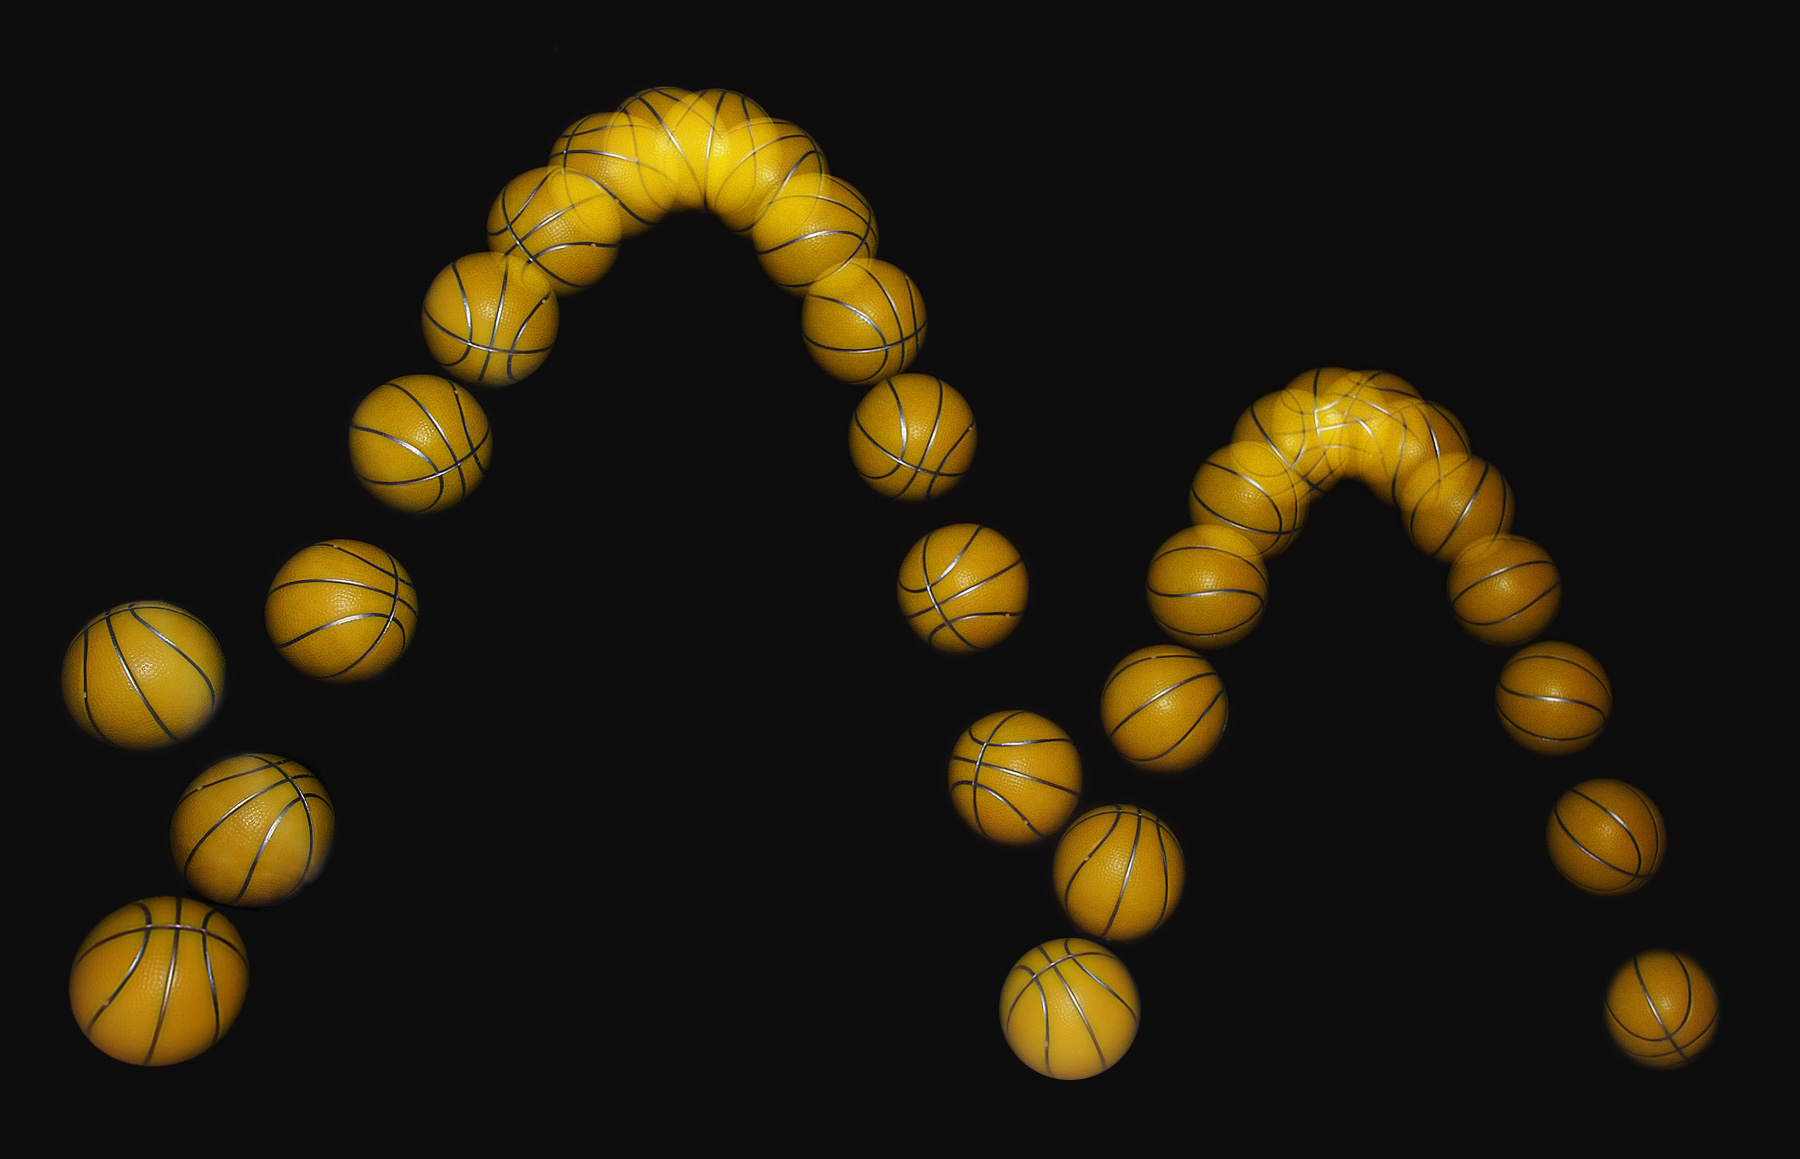
\includegraphics[width=1\linewidth]{src/images/bouncing_ball_strobe_edit.jpg}
\end{sbspanel}
\end{sidebyside}
\begin{sidebyside}{2}{0.025}{0.025}{0.05}
\begin{sbspanel}{0.5}
\hypertarget{p-109}{}%
The graph shows the rebound height on the vertical axis and bounce number on the horizontal. Sketch a graph of the associated explicit function \(h(t)=3(0.75)^t\) where \(h(t)\) is the height at time \(t\). Explain how the graph you sketch is related to the discrete graph that is shown.%
\end{sbspanel}
\begin{sbspanel}{0.4}
\resizebox{\linewidth}{!}{{
\begin{tikzpicture}
\begin{axis}[
axis line style = {<->},
width = 0.5\linewidth,
xlabel = Number of Bounces,
y label style={at={(axis description cs:0,.5)}},
ylabel = Rebound Height (meters),
label style={font=\tiny},
xmin = -2, xmax = 8,
ymin = -0.2, ymax = 3.25,
ytick = {0, .25, ...,3},
xtick = {0, 1, ...,7},
tick label style={font=\tiny},
]

\addplot[only marks, color=blue] coordinates {
(0,  3)
(1,  2.25)
(2,  1.6875)
(3,  1.265625)
(4,  0.94921875)
(5,  0.711914063)
(6,  0.533935547)
(7, 0.40045166)
};

\end{axis}
\end{tikzpicture}
}
}
\end{sbspanel}
\end{sidebyside}
\end{divisionexercise}%
\begin{divisionexercise}{2}\hypertarget{exercise-19}{}
\hypertarget{p-110}{}%
In \hyperref[example-fading-blue-jeans]{Example~1} we used the recursive system \(C_0=1, C_n = 0.98C_{n-1}\) to represent the amount of color left in blue jeans after \(n\) washings. The graph shows remaining color on the vertical axis and number of washings on the horizontal axis. Sketch a graph of the associated explicit function \(C(t)=1(0.98)^t\) where \(t\) represents elapsed time.  Write a few sentences to explain how and why your graph differs from the discrete graph shown.%
\begin{figure}
\centering
{
\begin{tikzpicture}
\begin{axis}[
axis line style = {<->},
width = 0.5\linewidth,
xlabel = Number of Washes,
y label style={at={(axis description cs:0,.5)}},
ylabel = Percent Color Remaining,
label style={font=\tiny},
xmin = -2, xmax = 15,
ymin = -0.2, ymax = 1.2,
ytick = {0, .2, ...,1},
xtick = {0, 1, ...,14},
tick label style={font=\tiny},
]

\addplot[only marks, color=blue] coordinates {
(0,  1)
(1,  0.98)
(2,  0.9604)
(3,  0.941192)
(4,  0.92236816)
(5,  0.903920797)
(6,  0.885842381)
(7,  0.868125533)
(8,  0.850763023)
(9,  0.833747762)
(10,  0.817072807)
(11,  0.800731351)
(13,  0.769022389)
(12,  0.784716724)
(14,  0.753641941)
};

\end{axis}
\end{tikzpicture}
}
\caption{\label{figure-5}}
\end{figure}
\end{divisionexercise}%
\begin{example}\label{example-recursive-salary}
\hypertarget{p-111}{}%
Rebecca starts working for a company at a salary of \(\$40,000\) per year. Based on the company's history, she can expect raises of \(3.5\%\) each year on the anniversary of her employment. When will she first make \(\$50,000\)?%
\par\smallskip%
\noindent\textbf{Solution}.\hypertarget{solution-9}{}\quad%
\hypertarget{p-112}{}%
We can use the recursive system \(A_0=40,000, A_n=1.035A_{n-1}, n=1,2,3,...\) to determine when her salary will equal or exceed \(\$50,000\).  Rebecca’s first pay raise will result in a salary of \(\$41,400\).  Her sixth raise will bring her salary up to \(\$49,170.21\) and her seventh raise will put her pay over \(\$50,000\) at \(\$50,891.17\).%
\par
\hypertarget{p-113}{}%
We could also use a closed form function to solve for the time at which her salary will reach \(\$50,000\).  This function is \(S(t)=40,000(1.035)^t\). By evaluating this function, we find that \(S(6)=49,170.21\) and \(S(7)=50,891.17\). Both the recursive model and the closed form model inform us that Rebecca will make more than \(\$50,000\) with her \(7^{th}\) raise.%
\par
\hypertarget{p-114}{}%
If we wanted to know what Rebecca would make if she stayed with this company for \(30\) years, it would be easier to use the closed form and substitute \(t=30\).  In many cases either the recursive system or the closed form could be used to arrive at the same answer. In cases where we need to predict far into the future, it is more efficient to use the closed form. In cases where we want to see all of the intermediate values, as would be the case for the balance due on a loan after each payment, it would be to our advantage to use the recursive system. In Rebecca's case, if we choose to use an explicit representation we must limit the domain to integer values since her pay raises occur only one time per year.%
\end{example}
\begin{example}[{Doubling Time.}]\label{example-doubling-time}
\hypertarget{p-115}{}%
Suppose the population of a certain type of bacteria is known to grow geometrically and increases by about \(26\%\) every hour. How much time will it take for a population of \(150\) million cells to grow to \(300\) million? How long will it take the population to double again to \(600\) million? When will the population reach \(1200\) million (another doubling)?%
\par\smallskip%
\noindent\textbf{Solution}.\hypertarget{solution-10}{}\quad%
\hypertarget{p-116}{}%
Since the population is growing by \(26\%\) per hour, we can use the recursive system%
%
\begin{gather*}
P_0 = 150, P_n = (1.26)P_{n-1}
\end{gather*}
\hypertarget{p-117}{}%
We also have the option of using the explicit function \(P(t)=150 \cdot (1.26)^t\).  For integer values of \(t\), these two representations give roughly identical values for the number of bacteria cells.%
\begin{sidebyside}{2}{0}{0}{0}
\begin{sbspanel}{0.5}
{\centering%
\begin{tabular}{ll}
\multicolumn{1}{lB}{Time (Hours)}&Cells (Millions)\tabularnewline\hrulethick
\multicolumn{1}{lB}{\(0\)}&\(150\)\tabularnewline\hrulemedium
\multicolumn{1}{lB}{\(1\)}&\(189\)\tabularnewline\hrulemedium
\multicolumn{1}{lB}{\(2\)}&\(238.14\)\tabularnewline\hrulemedium
\multicolumn{1}{lB}{\(3\)}&\(300.06\)\tabularnewline\hrulemedium
\multicolumn{1}{lB}{\(4\)}&\(378.07\)\tabularnewline\hrulemedium
\end{tabular}
\par}
\end{sbspanel}
\begin{sbspanel}{0.5}
{\centering%
\begin{tabular}{ll}
\multicolumn{1}{lB}{Time (Hours)}&Cells (Millions)\tabularnewline\hrulethick
\multicolumn{1}{lB}{\(5\)}&\(476.37\)\tabularnewline\hrulemedium
\multicolumn{1}{lB}{\(6\)}&\(600.22\)\tabularnewline\hrulemedium
\multicolumn{1}{lB}{\(7\)}&\(756.28\)\tabularnewline\hrulemedium
\multicolumn{1}{lB}{\(8\)}&\(952.92\)\tabularnewline\hrulemedium
\multicolumn{1}{lB}{\(9\)}&\(1200.67\)\tabularnewline\hrulemedium
\end{tabular}
\par}
\end{sbspanel}
\end{sidebyside}
\par
\hypertarget{p-118}{}%
The population took about \(3\) hours to double from \(150\) to \(300\) million.  In another \(3\) hours, it had doubled again, and in another \(3\) hours there was yet another population doubling. This population is said to have a \emph{doubling time} of \(3\) hours. Note that the first doubling corresponds to an increase of \(150\) cells, the next doubling is an increase of \(300\) cells, and the third doubling is an increase of \(600\) cells. For each of these doublings, the elapsed time is the same (\(3\) hours) but the increase, measured in cells per hour, is not the same.%
\end{example}
\hypertarget{p-119}{}%
Example \hyperref[example-doubling-time]{10} shows that a population that experiences geometric growth has a doubling time. It is also true that populations that experience geometric decay have a \emph{half-life}. A half-life is the amount of time it takes for a population size to be halved. Populations that experience other types of growth, such as linear, quadratic or logistic, do not have a doubling time.%
\par
\hypertarget{p-120}{}%
The exponential function you studied in Chapter 2, \(f(t)=2^t\), has a doubling time of \(1\) time unit. This is because%
%
\begin{align*}
f(1)&=2^1=2\\
f(2)&=2^2=4\\
f(3)&=2^3=8\\
f(4)&=2^4=16
\end{align*}
\hypertarget{p-121}{}%
A doubling of function-values takes place with each increase of \(1\) unit in \(t\)%
\par
\hypertarget{p-122}{}%
The function \(g(t)=2^{\frac{1}{3} t}\) is a horizontal stretch of the function \(f(t)=2^t\), and this transformation makes \(g(t)\) have a doubling time of \(3\) time units:%
%
\begin{align*}
g(3)&=2^{\frac{1}{3} \cdot 3}=2^1=2\\
g(6)&=2^{\frac{1}{3} \cdot 6}=2^2=4\\
g(9)&=2^{\frac{1}{3} \cdot 9}=2^3=8
\end{align*}
\hypertarget{p-123}{}%
Since \(g(t)=2^{\frac{1}{3} t}\) has a doubling time of \(3\) time units, in Example \hyperref[example-doubling-time]{10} we could have used the function \(y = 150 \cdot 2^{\frac{1}{3} t}\) to model the number of bacteria cells present at time \(t\). You can confirm that the two functions \(y = 150 \cdot 2^{\frac{1}{3} t}\) and \(P(t)=150 \cdot (1.26)^t\) produce roughly the same ordered pairs.%
\typeout{************************************************}
\typeout{Exercises 4.3.2 Exercises}
\typeout{************************************************}
\subsection[{Exercises}]{Exercises}\label{exercises-5}
\hypertarget{exercisegroup-1}{}
\par\noindent \hypertarget{p-124}{}%
In exercises \(1\) through \(4\), identify whether the growth (or decay) that is described is discrete or continuous.  Write either a recursive system or an expliciit function to represent the phenomenon. Use the most appropriate form to answer each question.%
\begin{exercisegroup}{1}
\begin{egexercise}{1}\hypertarget{exercise-20}{}
\hypertarget{p-125}{}%
Research City is growing by \(14\%\) each year.  If the population of the city is approximately one million people and the rate of growth continues at \(14\%\) annually, what will Research City's population be \(15\) years from now?%
\end{egexercise}%
\begin{egexercise}{2}\hypertarget{exercise-21}{}
\hypertarget{p-126}{}%
The population of Coastal City grows by \(3\%\) each year due only to births and deaths among current residents.  The population is currently one million.  Each year \(15,000\) more people move into the city than move out, resulting in a net gain of \(0.015\) milion people. How long will it take Coastal City's population to reach \(1.8\) million people?%
\end{egexercise}%
\begin{egexercise}{3}\hypertarget{exercise-22}{}
\hypertarget{p-127}{}%
Each year hunting and natural predators combine to cause the population of rabbits in the meadow to decrease by \(5\%\).  If the year begins with \(230\) rabbits and the population continues to decrease by \(5\%\) each year, how many rabbits will there be in this meaudow in \(50\) years?%
\end{egexercise}%
\begin{egexercise}{4}\hypertarget{exercise-23}{}
\hypertarget{p-128}{}%
Each year the population of rabbits in the meadow decreases by \(5\%\).  Farmer Dan decides to help the rabbit population by releasing \(5\) new rabbits into the meadow each year.  If the year begins with \(230\) rabbits, describe what will happen to the population over the next ten years.%
\end{egexercise}%
\end{exercisegroup}
\par\noindent%
\par\medskip\noindent
\begin{divisionexercise}{5}\hypertarget{exercise-24}{}
\hypertarget{p-129}{}%
An annual inflation rate of \(k\%\) means that items will cost \(k\%\) more next year than they cost this year.  Based on a yearly inflation rate of \(3\%\), estimate the cost of the following items in \(10\), \(20\), \(30\), and \(40\) years.%
\begin{table}
\centering
\begin{tabular}{ll}
\multicolumn{1}{lB}{Item}&Cost Today\tabularnewline\hrulethick
\multicolumn{1}{lB}{Jeans}&\(\$45.00\)\tabularnewline\hrulemedium
\multicolumn{1}{lB}{Hamburger}&\(\$3.90\)\tabularnewline\hrulemedium
\multicolumn{1}{lB}{Car}&\(\$29,000\)\tabularnewline\hrulemedium
\multicolumn{1}{lB}{Textbook}&\(\$75.00\)\tabularnewline\hrulemedium
\multicolumn{1}{lB}{Movie Ticket}&\(\$9.00\)\tabularnewline\hrulemedium
\end{tabular}
\caption{Cost of Items\label{table-6}}
\end{table}
\end{divisionexercise}%
\begin{divisionexercise}{6}\hypertarget{exercise-25}{}
\hypertarget{p-130}{}%
How much money would you need to invest now in an account that receives \(0.5\%\) monthly interest so that in \(20\) years you will have \(\$50,000\)?%
\end{divisionexercise}%
\begin{divisionexercise}{7}\hypertarget{exercise-26}{}
\hypertarget{p-131}{}%
The number of cells in a certain bacteria colony triples every hour.  Write an explicit function that models this growth.  By what factor does the population grow in half an hour?%
\end{divisionexercise}%
\begin{divisionexercise}{8}\hypertarget{exercise-27}{}
\hypertarget{p-132}{}%
Thorieum-\(234\) is a radioactive material whose half-life is \(25\) days. Write an explicit function for the amount of thorium-\(234\) left after \(t\) days.  What percent of an original amount is left after \(300\) days?%
\end{divisionexercise}%
\begin{divisionexercise}{9}\hypertarget{exercise-28}{}
\hypertarget{p-133}{}%
The population of The Peoples Republic of China in \(2015\) was a little over \(1.39\) billion and growing at a rate of about \(0.5\%\) annually. \leavevmode%
\begin{enumerate}[label=(\alph*)]
\item\hypertarget{li-58}{}Write a recursive system to model the population%
\item\hypertarget{li-59}{}Find an explicit function to model the population%
\item\hypertarget{li-60}{}To the nearest year, how long will it take the population to double? Assume that the growth rate remains \(0.5\%\) per year.%
\item\hypertarget{li-61}{}Use the doubling time you found in part (c) to write an transformation of the function \(y=2^x\) to represent China's population. (Use \(x\) to represent the number of years elapsed since \(2015\).).%
\item\hypertarget{li-62}{}Write a few sentences to compare and contrast the models you found in parts a, b, and d.%
\end{enumerate}
%
\end{divisionexercise}%
\begin{divisionexercise}{10}\hypertarget{exercise-29}{}
\hypertarget{p-134}{}%
When you are \(40\) years old your rich Uncle Harry leaves you \(\$10,000\) in his will when he dies.  His death makes you realize it is time to start saving for your own retirement. Your goal is to deposit enough in a retirement account when you are between the ages of \(40\) and \(65\) that you can "pay yourself" a comfortable amount each year when you are over \(65\). \leavevmode%
\begin{enumerate}[label=(\alph*)]
\item\hypertarget{li-63}{}On your \(40^{th}\) birthday you invest the \(\$10,000\) in an account that pays \(3.5\%\) annual interest.  You also decide to make a yearly deposit in the account of \(\$1,000\). What will your balance be when you turn \(65\)?  Give the amount in your account when you turn \(65\) and write the equations you use to arrive at your answer.%
\item\hypertarget{li-64}{}Will you have enough money in your account when you are \(65\) to pay yourself \(\$5,000\) per year from age \(65\) to age \(80\).  While you are withdrawing money, the balance in the account continues to earn \(3.5\%\) annual interest.  Give a yes or no answer and write the equations you use to support your answer.%
\end{enumerate}
%
\end{divisionexercise}%
\begin{divisionexercise}{11}\hypertarget{exercise-30}{}
\hypertarget{p-135}{}%
Thomas has two plans for saving to buy a car.  In Plan A, he will make an initial deposit of \(\$50\) and then he will deposit \(\$33\) each week in an account that earns \(0.1\%\) interest per week.  In Plan B, he will make an initial deposit of \(\$50\) and then each week he will put \(\$30\) in an account that earns \(0.45\%\) each week. Write recursive equations to show the amounts Thomas would have under each of the plans. Write down the account balances under each plan during weeks \(1 - 3\) and during weeks \(50 - 52\)%
\end{divisionexercise}%
\begin{divisionexercise}{12}\hypertarget{exercise-31}{}
\hypertarget{p-136}{}%
In this section you have seen that the recursive system \(P_0=a, P_n=(1+k) \cdot P_{n-1}, n = 1, 2, 3, ...\) can be written as a closed form exponential function \(P(n)=a \cdot (1+k)^n\). What recursive system can be written as a closed form linear function of the form \(y(n)=a+kn\)?%
\end{divisionexercise}%
\typeout{************************************************}
\typeout{Section 4.4 Summing Geometric Growth}
\typeout{************************************************}
\section[{Summing Geometric Growth}]{Summing Geometric Growth}\label{chapter04-section04}
\hypertarget{p-137}{}%
In \(2012\) the world wide rate of crude oil consumption was about \(89,837\) thousand barrels per day and was increasing at an annual rate of about \(1.42\%\) \footnote{SOURCE: www.eia.gov\label{fn-1}}.  As a consequence, the world consumed about \(32.8\) billion barrels of crude oil in \(2012\) and about \(33.3\) billion barrels in \(2013\).  We can use the explicit function \(A(n)=32.8(1.0142)^n\), where \(n\) represents the number of years since \(2012\), to find that the amount of oil consumed in \(2042\) will be a little over \(50\) billion barrels, since \(A(30)=32.8(1.0142)^30 = 50.07\).  That is certainly a large amount, but knowing the amount in any one year does not really tell the whole story.  A more important question:  What is the total amount of crude oil that will be consumed between \(2012\) and \(2042\)?  This total represents the quantity of oil that will be depleted from world oil reserves over this \(31\)-year time period.%
\par
\hypertarget{p-138}{}%
To determine the total amount of oil consumed from \(2012\) to \(2042\), we want to find the sum:%
\begin{gather*}
T=A(0)+A(1)+A(2)+...+A(30)
\end{gather*}
%
\par
\hypertarget{p-139}{}%
We can rewrite the equation for \(T\) as:%
\begin{gather*}
T=32.8+32.8(1.0142)+32.8(1.0142)^2+...+32.8(1.0142)^{30}
\end{gather*}
%
\par
\hypertarget{p-140}{}%
Notice that each term in the sum is \(1.0142\) times the previous term. This sum is an example of a geometric series, which is a sum in which each successive addend is found by multiplying the previous term by some fixed value. Or, put another way, a geometric series is the sum of a geometric sequence.%
\par
\hypertarget{p-141}{}%
A more general way to represent a geometric series is:%
\begin{gather}
S = a + ar + ar^2 + ar^3 + ... + ar^n\label{chapter04-section04-geoseries-step1}
\end{gather}
%
\par
\hypertarget{p-142}{}%
This series has first term a and each subsequent term is obtained from the preceding term by multiplying by \(r\). The ratio of two consecutive terms in a geometric series is always \(r\), so r is known as the common ratio.%
\par
\hypertarget{p-143}{}%
We can find a formula for the sum of a geometric series without actually adding all of the terms, instead we use algebra in a clever way.  First, we multiply both sides of equation (1) by \(r\), which yields:%
\begin{gather}
Sr = ar + ar^2 + ar^3 + ar^4 + ... + ar^{n+1}\label{chapter04-section04-geoseries-step2}
\end{gather}
%
\par
\hypertarget{p-144}{}%
Most of the terms on the right sides of equations \hyperref[chapter04-section04-geoseries-step1]{(\ref{chapter04-section04-geoseries-step1})} and \hyperref[chapter04-section04-geoseries-step2]{(\ref{chapter04-section04-geoseries-step2})} are the same.  If we now subtract equation \hyperref[chapter04-section04-geoseries-step2]{(\ref{chapter04-section04-geoseries-step2})} from equation \hyperref[chapter04-section04-geoseries-step1]{(\ref{chapter04-section04-geoseries-step1})}, meaning we subtract the left side of \hyperref[chapter04-section04-geoseries-step2]{(\ref{chapter04-section04-geoseries-step2})} from the left side of \hyperref[chapter04-section04-geoseries-step1]{(\ref{chapter04-section04-geoseries-step1})} and the same with the right sides, we obtain the new equation:%
\begin{gather*}
S-Sr = a - ar^{n+1}
\end{gather*}
%
\par
\hypertarget{p-145}{}%
Solving this equation to isolate \(S\), we have:%
\begin{gather}
S = \frac{a-ar^{n+1}}{1-r}\label{chapter04-section04-geoseries-step3}
\end{gather}
%
\par
\hypertarget{p-146}{}%
Equation \hyperref[chapter04-section04-geoseries-step3]{(\ref{chapter04-section04-geoseries-step3})} represents the sum of the terms \(a\) through \(ar^n\) of a geometric series with first term \(a\) and common ratio \(r\), assuming \(r \neq 1\).%
\par
\hypertarget{p-147}{}%
Note that if \(r=1\) the series%
\begin{gather*}
S = a + ar + ar^2 + ar^3 + ... + ar^n
\end{gather*}
is equivalent to%
\begin{gather*}
S = a + a + a + a + ... + a
\end{gather*}
and the sum of this series is simply \(S=(n+1)a\)%
\par
\hypertarget{p-148}{}%
Returning to the question regarding world crude oil consumption from \(2012\) through \(2042\), we need to find the sum of terms \(0\) through \(30\) of a geometric series with initial term \(32.8\) and common ratio \(1.0142\) .  This sum is given by%
\begin{gather*}
T = \frac{32.8-32.8(1.0142)^{31}}{1-(1.0142)} \approx 1,266 \text{ billion barrels of oil} 
\end{gather*}
%
\par
\hypertarget{p-149}{}%
In the world’s top \(17\) oil producing countries, estimates of the total proven oil reserves that are recoverable with \(2012\) technology are in the range of \(1200\) to \(1300\) billion barrels.  Therefore, if oil consumption continues to increase at the rate observed in \(2012\), proven oil reserves will be almost exhausted by \(2042\).%
\par
\hypertarget{p-150}{}%
You will encounter a wide variety of situations in mathematics classes and in other disciplines that require finding the sum of a geometric series. This happens frequently enough that you should be sure to include in the collection of mathematical tools you have available to you either the formula for the sum of a geometric series, or the method used here to arrive at that sum.%
\par
\hypertarget{p-151}{}%
Below are two additional examples from the financial world where this concept is used.%
\begin{example}[{Value of an Annuity.}]\label{value-on-an-annuity}
\hypertarget{p-152}{}%
Suppose your parents want to set aside money for college tuition for a younger sibling.  They begin saving when she is twelve by opening an account with an initial deposit of \(\$100\).  At the beginning of each month for six years thereafter, they deposit an additional \(\$100\).  An account into which regular payments are made (or from which regular withdrawals are made) is called \emph{an annuity}.  The account into which they place the money earns \(0.5\%\) monthly interest, which is added to the account at the end of each month.  How much money will be in the account at the end of six years?%
\par\smallskip%
\noindent\textbf{Solution}.\hypertarget{solution-11}{}\quad%
\hypertarget{p-153}{}%
The initial deposit earns interest for \(72\) months, which means that in \(72\) months the first \(\$100\) deposited has grown to a value of \(\$100(1.005)^{72}\).  The money deposited at the beginning of the second month earns interest for \(71\) months and grows to \(\$100(1.005)^{71}\).  Each successive deposit earns interest for one month less than the previous deposit.  We will assume that your parents close the account on the day that they make the final payment of \(\$100\); this means that the final \(\$100\) deposit earns no interest.  The timeline in \hyperref[deposit-timeline]{Figure~2} shows each deposit together with the amount of interest earned by each deposit.%
\begin{figure}
\centering
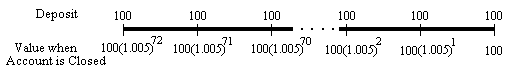
\includegraphics[width=0.8\linewidth]{src/images/chapter04-section04-depositchart.png}
\caption{Timeline for interest and deposit in an annuity (REDO GRAPHIC)\label{deposit-timeline}}
\end{figure}
\hypertarget{p-154}{}%
The balance of the annuity after six years is the sum of the values of all 73 deposits, which is%
\begin{gather*}
B = 100 + 100(1.005) + 100(1.005)^2 + 100(1.005)^3 + ... + 100(1.005)^{72}
\end{gather*}
This is a geometric series with initial term \(100\) and common ratio \(1.005\), so we can use equation \hyperref[chapter04-section04-geoseries-step3]{(\ref{chapter04-section04-geoseries-step3})} to write the sum of this series as%
\begin{gather}
B= \frac{100-100(1.005)^{73}}{1-1.005}\label{mrow-80}
\end{gather}
which equals \(\$8,784.09\), the balance of the annuity after six years.  Note that only \(\$7,300\) was deposited, so over \(6\) years the deposits have earned over \(\$1,400\) in interest.%
\end{example}
\begin{example}[{Paying Off a Loan.}]\label{example-12}
\hypertarget{p-155}{}%
Suppose you borrow \(\$20,000\) to buy a car, and you agree to pay back the loan over \(48\) months at \(0.4 \%\) interest per month.  You want to determine the monthly payment \(P\) that you must make in order to pay off the loan. You know how to find the payment using a "guess and check" method.  Now, since you are able to find the sum of a geometric series, you can write and solve an equation to find the payment.%
\par\smallskip%
\noindent\textbf{Solution}.\hypertarget{solution-12}{}\quad%
\hypertarget{p-156}{}%
Your outstanding balance can be represented with the recursive system%
%
\begin{gather*}
L_0=20,000, L_n=1.004L_{n-1}-P, n=1,2,3,...
\end{gather*}
\hypertarget{p-157}{}%
Where \(L_n\) is the amount still owed on the loan after \(n\) months and \(P\) is the monthly payment in dollars.  We know that after one month,%
%
\begin{gather*}
L_1=1.004(20,000)-P
\end{gather*}
\hypertarget{p-158}{}%
After two months, the amount still owed is given by%
%
\begin{gather*}
L_2 = 1.004L_1-P
\end{gather*}
\hypertarget{p-159}{}%
which, by substitution is equivalent to%
%
\begin{align*}
L_2&=1.004(1.004 \cdot 20,000 - P) - P\\
\text{or}\\
L_2&=1.004^2(20,000)-1.004P-P
\end{align*}
\hypertarget{p-160}{}%
Similarly, since \(L_3=1.004L_2-P\), we have:%
%
\begin{align*}
L_3&=1.004(1.004^2 (20,000) - 1.004P - P) - P\\
L_3&=1.004^3(20,000) - 1.004^2P - 1.004P - P
\end{align*}
\hypertarget{p-161}{}%
We can continue to iterate to find the outstanding balance after any number of months. For instance,%
%
\begin{gather*}
L_5=1.004^5 (20,000)-1.004^4 P-1.004^3 P-1.004^2 P-1.004P-P
\end{gather*}
\hypertarget{p-162}{}%
In general, we see that after \(n\) months the oustanding balance is given by:%
%
\begin{gather}
L_n=1.004^n (20,000) - P \big( 1.004^{n-1} + 1.004^{n-2} + ... + 1.004^2 + 1.004 + 1 \big)\label{general-annuity-formula-long}
\end{gather}
\hypertarget{p-163}{}%
Embedded in the right side of equation \hyperref[general-annuity-formula-long]{(\ref{general-annuity-formula-long})} is the geometric series%
%
\begin{gather*}
1 + 1.004 + 1.004^2 + 1.004^3 + ... + 1.004^{n-2} + 1.004^{n-1}
\end{gather*}
\hypertarget{p-164}{}%
which has first term \(1\) and common ratio \(1.004\). Using equation \hyperref[chapter04-section04-geoseries-step3]{(\ref{chapter04-section04-geoseries-step3})}, we know that%
%
\begin{gather*}
1 + 1.004 + 1.004^2 + 1.004^3 + ... + 1.004^{n-2} + 1.004^{n-1} = \frac{1-1.004^n}{1-1.004}
\end{gather*}
\hypertarget{p-165}{}%
Substituting into equation \hyperref[general-annuity-formula-long]{(\ref{general-annuity-formula-long})} we obtain the following representation for  \(L_n\):%
%
\begin{gather}
L_n = 1.004^n (20,000) - P\bigg(\frac{1-1.004}{1-1.004^n}\bigg)\label{general-annuity-formula-condensed}
\end{gather}
\hypertarget{p-166}{}%
We want \(48\) payments to reduce the outstanding balance to zero, that is, our goal is  \(L_{48}=0\). This means that we can solve the following equation to find the value of \(P\).%
%
\begin{gather*}
0 = 1.004^{48}(20,000)-P\bigg(\frac{1-1.004^{48}}{1-1.004}\bigg)
\end{gather*}
\hypertarget{p-167}{}%
Solving for \(P\), we find%
%
\begin{align*}
P &= 1.004^{48}(20,000)\bigg(\frac{1-1.004^{48}}{1-1.004}\bigg)\\
\text{or, equivalently}\\
P&=\frac{1.004^{48}(20,000)(0.004)}{1.004^{48}-1}
\end{align*}
\hypertarget{p-168}{}%
which means that \(P \approx 458.78\). The loan will be paid off in \(48\) months with a monthly payment of \(\$458.78\). You should verify using the recursive system%
%
\begin{gather*}
L_0 = 20,000, L_n = 1.004L_{n-1}, n = 1, 2, 3, ...
\end{gather*}
\hypertarget{p-169}{}%
that the balance after \(48\) payments, \(L_{48}\) is zero. Note that due to rounding, your answer may not be exactly zero. The final baloon payment may be a few cents more or less than \(\$458.78\)%
\par
\hypertarget{p-170}{}%
It is worthwhile to take a moment to study equation \hyperref[general-annuity-formula-condensed]{(\ref{general-annuity-formula-condensed})}, which effectively gives an explicit function for \(L(n)\).%
%
\begin{gather*}
L(n) = 1.004^n (20,000) - P \bigg(\frac{1-1.004^n}{1-1.004}\bigg)
\end{gather*}
\hypertarget{p-171}{}%
Recall that the monthly interest rate was \(0.4\%\), the amount borrowed was \(\$20,000\),  \(L(n)\) is the amount still owed after \(n\) payments, and \(P\) is the monthly payment. You should conclude that if the monthly interest rate is k\% and the amount borrowed is \(\$A\), then \(L(n)\), the amount still owed after \(n\) payments, will be given by%
%
\begin{gather}
L(n) = (1+k)^n A - P \bigg(\frac{1-(1+k)^n}{1-(1+k)}\bigg)\label{mrow-100}
\end{gather}
\hypertarget{p-172}{}%
If you want the outstanding balance to be zero after \(n^*\) months, you can solve to find the value of \(P\) for which \(L(n^*)=0\).%
\end{example}
\typeout{************************************************}
\typeout{Exercises 4.4 Exercises}
\typeout{************************************************}
\subsection*{Exercises}\hypertarget{exercises-6}{}
\addcontentsline{toc}{subsection}{Exercises}
\begin{divisionexercise}{1}\hypertarget{exercise-32}{}
\hypertarget{p-173}{}%
Consider the geometric series \(100+100(1.05)+100(1.05)^2+100(1.05)^3+...\)%
\leavevmode%
\begin{enumerate}[label=(\alph*)]
\item\hypertarget{li-65}{}Find the sum of the first \(10\) terms of the series%
\item\hypertarget{li-66}{}Find the sum of the first \(100\) terms of the series%
\item\hypertarget{li-67}{}Find the sum of the first \(500\) terms of the series%
\end{enumerate}
\end{divisionexercise}%
\begin{divisionexercise}{2}\hypertarget{exercise-33}{}
\hypertarget{p-174}{}%
Consider the geometric series \(200+200(0.8)+200(0.8)^2+200(0.8)^3+...\)%
\leavevmode%
\begin{enumerate}[label=(\alph*)]
\item\hypertarget{li-68}{}Find the sum of the first \(50\) terms of the series%
\item\hypertarget{li-69}{}Find the sum of the first \(500\) terms of the series%
\item\hypertarget{li-70}{}Find the sum of the first \(1000\) terms of the series%
\item\hypertarget{li-71}{}Make a prediction about the sum of the first million terms. Compare your prediction with the actual sum.%
\end{enumerate}
\end{divisionexercise}%
\begin{divisionexercise}{3}\hypertarget{exercise-34}{}
\hypertarget{p-175}{}%
Consider the geometric series \(3+1.5+0.75+0.375+...\)%
\leavevmode%
\begin{enumerate}[label=(\alph*)]
\item\hypertarget{li-72}{}Find the sum of the first \(10\) terms of the series%
\item\hypertarget{li-73}{}Find the sum of the first \(50\) terms of the series%
\item\hypertarget{li-74}{}How many terms of the series must be added to bring the sum to at least \(5.99999\)?%
\end{enumerate}
\end{divisionexercise}%
\begin{divisionexercise}{4}\hypertarget{exercise-35}{}
\hypertarget{p-176}{}%
Consider the geometric series with first term \(\frac{9}{10}\) and common ratio \(\frac{1}{10}\)%
\leavevmode%
\begin{enumerate}[label=(\alph*)]
\item\hypertarget{li-75}{}Find the sum of the first \(10\) terms of the series%
\item\hypertarget{li-76}{}Find the sum of the first \(100\) terms of the series%
\item\hypertarget{li-77}{}Explain if it is meaningful to talk about adding infinitely many of the terms in this series%
\end{enumerate}
\end{divisionexercise}%
\begin{divisionexercise}{5}\hypertarget{exercise-36}{}
\hypertarget{p-177}{}%
Let \(T(n)\) represent the sum of the first \(n\) terms of the series \(1 - \frac{1}{2} + \frac{1}{4} - \frac{1}{8} + ...\)%
\leavevmode%
\begin{enumerate}[label=(\alph*)]
\item\hypertarget{li-78}{}Find the sum of \(T(10)\) without actually adding terms.%
\item\hypertarget{li-79}{}Find an explicit expression for \(T(n)\) in terms of \(n\).%
\item\hypertarget{li-80}{}Describe how the values of \(T(n)\) behave as \(n\) increases without bound.%
\end{enumerate}
\end{divisionexercise}%
\begin{divisionexercise}{6}\hypertarget{exercise-37}{}
\hypertarget{p-178}{}%
Let \(T(n)\) represent the sum of the first \(n\) terms of the series \(0.3 + 0.03 + 0.003 + 0.0003 + ...\)%
\leavevmode%
\begin{enumerate}[label=(\alph*)]
\item\hypertarget{li-81}{}Find an explicit expression for \(T(n)\) in terms of \(n\).%
\item\hypertarget{li-82}{}Describe how the values of \(T(n)\) behave as \(n\) increases without bound.%
\end{enumerate}
\end{divisionexercise}%
\begin{divisionexercise}{7}\hypertarget{exercise-38}{}
\hypertarget{p-179}{}%
Let \(S(n)\) represent the sum of the first \(n\) terms of the series with common ratio \(r\). For what values of \(r\) is it meaningful to talk about adding infinitely many terms of the series?%
\end{divisionexercise}%
\begin{divisionexercise}{8}\hypertarget{exercise-39}{}
\hypertarget{p-180}{}%
Find the sum of each geometric series.%
\leavevmode%
\begin{enumerate}[label=(\alph*)]
\item\hypertarget{li-83}{}\(3 + 6 + 12 + ... + 192\)%
\item\hypertarget{li-84}{}\(1 + 0.2 + (0.2)^2 + (0.2)^3 + ... + (0.2)^14\)%
\item\hypertarget{li-85}{}\(4 + 4^2 + 4^3 + ... + 4^45\)%
\item\hypertarget{li-86}{}\(3 + \frac{3}{5} + \frac{3}{25} + \frac{3}{125} + ... + \frac{3}{5^{20}}\)%
\item\hypertarget{li-87}{}\(3 - \frac{3}{5} + \frac{3}{25} - \frac{3}{125} + ... + \frac{3}{5^{20}}\)%
\end{enumerate}
\end{divisionexercise}%
\begin{divisionexercise}{9}\hypertarget{exercise-40}{}
\hypertarget{p-181}{}%
In the oil consumption problem at the beginning of this section, the consumption of oil is increasing at a rate of \(1.42\%\) per year. By how many billions of barrels will the total consumption of oil from \(2012\) to \(2042\) be reduced if the rate of increase is reduced to \(1\%\)?%
\end{divisionexercise}%
\begin{divisionexercise}{10}\hypertarget{exercise-41}{}
\hypertarget{p-182}{}%
The number of new cars sold at a car dealer each year grows at a rate of \(1.5\%\) a year. This year, the dealer sold \(200\) cars. Assume that the \(1.5\%\) annual growth rate continues.%
\leavevmode%
\begin{enumerate}[label=(\alph*)]
\item\hypertarget{li-88}{}How many cars will the dealer sell \(15\) years from now%
\item\hypertarget{li-89}{}What is the total number of cars that will have been sold between this year and \(15\) years in the future?%
\end{enumerate}
\end{divisionexercise}%
\begin{divisionexercise}{11}\hypertarget{exercise-42}{}
\hypertarget{p-183}{}%
The landfill in Jefferson County can hold \(22.6\) million cubic yards of compacted garbage. In \(2015\) the city of Jefferson and the surrounding communities contributed \(550,000\) cubic yards of garbage to the landfill. The following year the total amount was about \(560,000\) cubic yards, which represents a \(1.8\%\) increase. This rate of Increase is actually smaller than the population growth rate of the county, so residents are reducing their per capita contributions to the land fill. \footnote{Adapted from Mathematics Modeling our Worlds COMAP course 2\label{fn-2}}%
\leavevmode%
\begin{enumerate}[label=(\alph*)]
\item\hypertarget{li-90}{}Find the total amount of garbage, in cubic yards, that the country residents will contribute to the landfill over the next \(10\) years, from \(2015\) thru \(2024\)%
\item\hypertarget{li-91}{}In what year will the landfill reach its capacity, if the annual growth rate of garbage volume remains at \(1.8\%\)?%
\item\hypertarget{li-92}{}Suppose that new recycling program can decrease the number of cubic yards of garbage that the country produces. In \(2015\) residents contributed \(550,000\) cubic yards of garbage to the landfill and annual rate of increase is brought down to \(1\%\).  How many years will the landfill last under these conditions?%
\item\hypertarget{li-93}{}How long would the landfill last if the annual rate of increase of garbage contribution was brought down to zero?%
\end{enumerate}
\end{divisionexercise}%
\begin{divisionexercise}{12}\hypertarget{exercise-43}{}
\hypertarget{p-184}{}%
You have an annuity to which you initially depot \(\$1,000\) and you add \(\$150\) each month. The account earns interest at \(0.35\%\) monthly interest rate; interest earned is added to the account balance at the end of each month.%
\leavevmode%
\begin{enumerate}[label=(\alph*)]
\item\hypertarget{li-94}{}Write a recursive model for the situation.%
\item\hypertarget{li-95}{}How much money will you have after \(3\) years?%
\item\hypertarget{li-96}{}How much money will you have after \(n\) months? Your answer should be written in the form of an explicit expression.%
\end{enumerate}
\end{divisionexercise}%
\begin{divisionexercise}{13}\hypertarget{exercise-44}{}
\hypertarget{p-185}{}%
Compare these two investment strategies to save for retirement by determining the account balance at age \(65\):%
\par
\hypertarget{p-186}{}%
\emph{Strategy I:} For the \(8\) years from age \(44\) to age \(52\), invest \(\$300\) per month and earn interest at a rate of \(0.75\%\) per month. Do not save any more money after age \(52\), and make no withdrawals from the account.%
\par
\hypertarget{p-187}{}%
\emph{Strategy II:} For the \(16\) years from age \(49\) to age \(65\), invest \(\$300\) per month and earn at a rate of \(0.75\%\) per month. Make no withdrawals from the account.%
\end{divisionexercise}%
\begin{divisionexercise}{14}\hypertarget{exercise-45}{}
\hypertarget{p-188}{}%
Start by writing an explicit function that expresses \(Y_n\) in terms of \(n\) if the values of \(Y_n\) are generated by the recursive system \(Y_0=A, Y_n=aY_{n-1}+b, n = 1, 2, 3, ...\) Use the method for summing a geometric series. Then:%
\leavevmode%
\begin{enumerate}[label=(\alph*)]
\item\hypertarget{li-97}{}Use your explicit function to determine the balance in an annuity after \(25\) years if an initial deposit of \(\$50,000\) and regular annual deposits of \(\$1,000\) have all earned interest at a \(3.5\%\) annual rate.%
\item\hypertarget{li-98}{}Use your explicit function to determine the outstanding balance after \(60\) months on a loan of \(\$55,000\) if payments of \(\$600\) are made each month and the interest rate is \(2.4\%\) per month.%
\end{enumerate}
\end{divisionexercise}%
\begin{divisionexercise}{15}\hypertarget{exercise-46}{}
\hypertarget{p-189}{}%
Earl and Larry are twins.  They both went to work at the age of \(24\) at the same job.  On their birthday each year (starting with their \(25^{\text{th}}\)birthday), they received identical bonuses of \(\$2,000\).  However, they decided to deal with their finances differently.\footnote{Adapted from: Smith, Keith, Tim and Tom's Financial Adventure, HIMap Pull-Out Section, COMAP Consortium, Fall, 1991\label{fn-3}}%
\par
\hypertarget{p-190}{}%
%
\par
\hypertarget{p-191}{}%
\emph{Earl's Strategy}: Earl decided to invest his money early in life, and each year, he took his bonus and put it in a savings account that earned \(6.6\%\) annual interest.  At the age of \(34\), Earl decided to live life a little and began spending his bonuses (beginning with the one he received at age \(35\)).  He did not, however, use any of the money he already had in his savings account.  He let it continue growing until He turned \(60\) years old, without depositing any new money into his savings account.%
\par
\hypertarget{p-192}{}%
%
\par
\hypertarget{p-193}{}%
\emph{Larry's Strategy:} Larry decided to have some fun when he was young and spent his bonuses up until he turned \(34\).  After he turned \(34\) and received his bonus, he realized that he should start thinking about the future and put some money away for retirement.  He began to invest his bonuses (starting with the one he received at age \(35\)) in a savings account that earned \(6.6\%\) annual interest.  He did this until the age of \(60\), including the bonus he received on his \(60^{\text{th}}\) birthday.%
\par
\hypertarget{p-194}{}%
%
\par
\hypertarget{p-195}{}%
Your task is to compare Earl's and Larry's investment strategies.  Your analysis should include the amount each twin has in his bank account on their \(60^{\text{th}}\) birthday as well as how much bonus money each twin was able to spend between the ages of \(25\) and \(60\).  Which investment strategy would you recommend?  Your comparison should include both \emph{recursive equations and explicit functions} that represent the amount of money Earl and Larry have in their respective accounts at any time.%
\end{divisionexercise}%
\typeout{************************************************}
\typeout{Section 4.5 Compound Interest (or the Magic of Compounding)}
\typeout{************************************************}
\section[{Compound Interest (or the Magic of Compounding)}]{Compound Interest (or the Magic of Compounding)}\label{chapter04-section05}
\hypertarget{p-196}{}%
In the previous section, we encountered a situation in which money was deposited into an interest-bearing account, and the interest was added to the account at regular intervals.  For example, suppose Maria deposits \(\$1,000\) in an account that earns interest at a rate of \(5\%\) annually.  After one year, the balance of the account will increase to \(\$1,050\).  After two years the balance will be \(\$1,102.50\) and so on according to the recursive equation%
%
\begin{gather*}
A_n = A_{n-1} + 0.05 A_{n-1}
\end{gather*}
\hypertarget{p-197}{}%
where \(A_n\) is the account balance after \(n\) years. \(A_n\) is known as the \emph{future value} of the initial deposit of \(\$1,000\) after \(n\) years.  The interest in Maria's account is \emph{compounded annually}, which means that the interest that has been earned during a year is credited to the account at the end of that year.%
\par
\hypertarget{p-198}{}%
Rather than adding earned interest into an account at the end of each year, financial institutions often use quarterly, monthly, or daily compounding.  For example, a bank that compounds monthly would add one month's interest into the account at the end of every month. As a consequence, during the second month, the initial deposit and the first month's interest will both earn interest.  During the third month, the initial deposit and two months of interest payments will earn interest.%
\par
\hypertarget{p-199}{}%
What effect does the frequency of compounding have on the future value of Maria's \(\$1,000\) deposit?  We will rely on the formula \(I=prt\), where \(I\) is the amount of interest earned in one compounding time period, \(p\) the principal, \(r\) the annual interest rate, and \(t\) the time (in years) between successive compoundings. We see that at the end of the first month, the amount of interest earned is \(I=1000 \cdot 0.05 \cdot 1/12 \approx 4.17\)  The account balance after one month is%
%
\begin{gather*}
\$1,000 + \$1,000(0.05) \frac{1}{12} = \$1,000 \bigg( 1 + \frac{0.05}{12}\bigg) = \$1,004.17
\end{gather*}
\hypertarget{p-200}{}%
At the end of the second month, the account has a balance of%
%
\begin{gather*}
\$1,004.17\bigg(1 + \frac{0.05}{12}\bigg) = \$1,008.35
\end{gather*}
\hypertarget{p-201}{}%
At the end of the third month, the account has a balance of%
%
\begin{gather*}
\$1,008.35 \bigg(1 + \frac{0.05}{12}\bigg) = \$1,012.55
\end{gather*}
\hypertarget{p-202}{}%
At the end of the first year, which contains twelve compounding periods, the balance will be%
%
\begin{gather*}
\$1,000 \bigg(1 + \frac{0.05}{12}\bigg)^{12} = \$1,051.16
\end{gather*}
\hypertarget{p-203}{}%
Notice that this amount is higher than the balance of \(\$1,050.00\) that we expect at the end of one year using annual compounding. This increased balance is the result of Maria earning interest on interest payments that have been deposited into the account during the year.%
\begin{example}[{Investment Accounts.}]\label{chapter04-section05-investment-accounts}
\hypertarget{p-204}{}%
Financial institutions often offer a variety of investment accounts from which their customers can choose.%
\leavevmode%
\begin{enumerate}
\item\hypertarget{li-99}{}What will be Felix’s account balance after \(1\) year if he deposits \(\$100\) in an account that pays \(5\%\) annual interest that is compounded quarterly? What annual interest rate, compounded only one time per year, would result in the same account balance?%
\item\hypertarget{li-100}{}What will be Felix’s account balance after \(1\) year if he deposits \(\$100\) in an account that pays \(4.9\%\) annual interest that is compounded daily? What annual interest rate, compounded only one time per year, would result in the same account balance?%
\item\hypertarget{li-101}{}Would Felix be better off investing money in an account that earns \(5.1\%\) annual interest that is compounded annually, or an account that earns \(5\%\) that is compounded every hour?%
\end{enumerate}
\par\smallskip%
\noindent\textbf{Solution}.\hypertarget{solution-13}{}\quad%
\leavevmode%
\begin{enumerate}
\item\hypertarget{li-102}{}If \(5\%\) annual interest is compounded quarterly (four times per year) then the account balance is multiplied by \((1+\frac{0.05}{4})\) each quarter. The account balance after \(n\) quarters is given by \(A(n)=100(1+\frac{0.05}{4})^n\). After \(1\) year, the balance will be \(A(4)=100(1+\frac{0.05}{4})^4 \approx \$105.09\). Felix would have ended up with the same account balance if he earned an interest rate of \(5.09\%\) that was compounded once per year.%
\item\hypertarget{li-103}{}When \(4.9\%\) annual interest is compounded daily (\(365\) times per year) the balance after \(n\) days is given by  \(A(n)=100(1+\frac{0.049}{365})^n\). After \(1\) year, the balance will be \(A(365) = 100(1+\frac{0.049}{365})^{365} \approx \$105.02\). An annual interest rate of \(5.02\%\) compounded once per year would have yielded the same balance as \(4.9\%\) compounded daily.%
\item\hypertarget{li-104}{}Felix can compare these accounts even if he does not know how much money he has to invest or how much time he will leave his money in the account.  Use \(A\) to represent his initial deposit.  If \(5.1\%\) interest is compounded once per year, his balance is multiplied by \((1.051)\) every year, and after \(n\) years his balance will be \(A(1.051)^n\) dollars. Now consider \(5\%\) annual interest being compounded every hour.  Since each compounding period is \(\frac{1}{8760}\) year, his balance is multiplied by \((1+\frac{0.05}{8760})\) every hour. Since there are \(8760\) hours in a year, the account balance is multiplied by \((1+\frac{0.05}{8760})^{8760}\) every year. Note that \((1 + \frac{0.05}{8760} )^{8760} \approx 1.0513\), so after \(n\) years Felix’s account balance will be \(A(1.0513)^n\) dollars. Felix is better off investing in the account that pays \(5\%\) interest compounded hourly because \(A(1.0513)^n > A(1.051)^n\) for all positive values of \(A\) and of \(n\).%
\end{enumerate}
\end{example}
\hypertarget{p-205}{}%
The different interest rates and compounding frequencies in \hyperref[chapter04-section05-investment-accounts]{Example~1} highlight the need for a way to compare these accounts. In part (a) we saw that \(5\%\) compounded quarterly has the same “effect” on an account balance as \(5.09\%\) compounded once per year. So we call \(5.09\%\) the \emph{effective annual yield}, or \emph{effective annual interest rate} of \(5\%\) compounded quarterly.  It is the interest rate that if compounded only once per year would yield the same balance as another rate with more frequent compounding. In part (b) we saw that \(4.8\%\) annual interest compounded daily has an effective annual yield of \(5.02\%\). In (c), we saw that \(5\%\) annual interest compounded once per hour has an effective annual yield of \(5.13\%\).%
\typeout{************************************************}
\typeout{Exercises 4.5.1 Class Practice}
\typeout{************************************************}
\subsection[{Class Practice}]{Class Practice}\label{exercises-7}
\begin{divisionexercise}{1}\hypertarget{chapter04-section05-classpractice-recursive-vs-explicit}{}
\leavevmode%
\begin{enumerate}[label=(\alph*)]
\item\hypertarget{li-105}{}Write a recursive system to represent the future value of an initial deposit \(A_0\) that earns \(r\%\) annual interest that is compounded quarterly. Let \(A_n\) represent the value after \(n\) years%
\item\hypertarget{li-106}{}Write an explicit function to represent the future value of an initial deposit \(A_0\) that earns \(r\%\) annual interest that is compounded quarterly. Let \(A(n)\) represent the value after \(n\) years%
\end{enumerate}
\end{divisionexercise}%
\begin{divisionexercise}{2}\hypertarget{exercise-48}{}
\hypertarget{p-206}{}%
Write representations as described in \hyperlink{chapter04-section05-classpractice-recursive-vs-explicit}{Exercise~1}, but use monthly compounding%
\end{divisionexercise}%
\begin{divisionexercise}{3}\hypertarget{exercise-49}{}
\hypertarget{p-207}{}%
Write representations as described in \hyperlink{chapter04-section05-classpractice-recursive-vs-explicit}{Exercise~1}, but use \(k\) compounding periods per year%
\end{divisionexercise}%
\hypertarget{p-208}{}%
\hyperref[impact-of-compounding-table]{Table~2} shows the future value of \(\$1,000\) earning \(5\%\) annual interest for various compounding frequencies. (All table entries are rounded to the nearest dollar.) You should be able to confirm the entries in the table.  For instance,%
%
\begin{gather*}
\$1,647 \approx \$1,000 \bigg( ( 1 + \frac{0.05}{12}) ^{12} \bigg)^{10} = \$1,000 \bigg( ( 1 + \frac{0.05}{12})^{120}\bigg)
\end{gather*}
\begin{table}
\centering
\begin{tabular}{llllllll}
\multicolumn{1}{cB}{}&\multicolumn{1}{cB}{Yearly}&\multicolumn{1}{cB}{Quarterly}&\multicolumn{1}{cB}{Monthly}&\multicolumn{1}{cB}{Weekly}&\multicolumn{1}{cB}{Daily}&\multicolumn{1}{cB}{Hourly}&\multicolumn{1}{c}{By the Minute}\tabularnewline[0pt]
\multicolumn{1}{cB}{Years (N)}&\multicolumn{1}{cB}{\(k=1\)}&\multicolumn{1}{cB}{\(k=4\)}&\multicolumn{1}{cB}{\(k=12\)}&\multicolumn{1}{cB}{\(k=52\)}&\multicolumn{1}{cB}{\(k=365\)}&\multicolumn{1}{cB}{\(k=8,760\)}&\multicolumn{1}{c}{\(k=525,600\)}\tabularnewline\hrulethick
\multicolumn{1}{lB}{1}&\multicolumn{1}{lB}{\(\$1,050\)}&\multicolumn{1}{lB}{\(\$1,051\)}&\multicolumn{1}{lB}{\(\$1,051\)}&\multicolumn{1}{lB}{\(\$1,051\)}&\multicolumn{1}{lB}{\(\$1,051\)}&\multicolumn{1}{lB}{\(\$1,051\)}&\(\$1,051\)\tabularnewline\hrulethick
\multicolumn{1}{lB}{10}&\multicolumn{1}{lB}{\(\$1,629\)}&\multicolumn{1}{lB}{\(\$1,634\)}&\multicolumn{1}{lB}{\(\$1,647\)}&\multicolumn{1}{lB}{\(\$1,648\)}&\multicolumn{1}{lB}{\(\$1,649\)}&\multicolumn{1}{lB}{\(\$1,649\)}&\(\$1,649\)\tabularnewline\hrulethick
\multicolumn{1}{lB}{25}&\multicolumn{1}{lB}{\(\$3,386\)}&\multicolumn{1}{lB}{\(\$3,463\)}&\multicolumn{1}{lB}{\(\$3,481\)}&\multicolumn{1}{lB}{\(\$3,488\)}&\multicolumn{1}{lB}{\(\$3,490\)}&\multicolumn{1}{lB}{\(\$3,490\)}&\(\$3,490\)\tabularnewline\hrulethick
\multicolumn{1}{lB}{50}&\multicolumn{1}{lB}{\(\$11,467\)}&\multicolumn{1}{lB}{\(\$11,495\)}&\multicolumn{1}{lB}{\(\$12,119\)}&\multicolumn{1}{lB}{\(\$12,168\)}&\multicolumn{1}{lB}{\(\$12,180\)}&\multicolumn{1}{lB}{\(\$12,182\)}&\(\$12,183\)\tabularnewline\hrulethick
\end{tabular}
\caption{Impact of the Frequency of Compounding\label{impact-of-compounding-table}}
\end{table}
\hypertarget{p-209}{}%
Reading down any column of \hyperref[impact-of-compounding-table]{Table~2}, we notice that the future value increases as the number of years increases.  This is to be expected. But reading across any row reveals that the future value seems to level off as the frequency of compounding increases.  For any number of years, there appears to be an upper limit to the future value of the account. We see that increasing the frequency of compounding is associated with an increase in the future value, but we don’t expect the future values associated with compounding “by the second” to be appreciably larger than the values displayed in the right-most column of the table for “by the minute” compounding.%
\par
\hypertarget{p-210}{}%
Each entry in \hyperref[impact-of-compounding-table]{Table~2} can be calculated with the explicit function%
%
\begin{gather*}
A(N)=1,000((1 + \frac{0.05}{k})^k)^N \text{or} A(N) = 1000(1 + \frac{0.05}{k})^{kN}
\end{gather*}
\hypertarget{p-211}{}%
where \(A(N)\) is the future value of \(N\) years.%
\par
\hypertarget{p-212}{}%
The value of \(N\) is fixed in each row of \hyperref[impact-of-compounding-table]{Table~2}, in the first row \(N=1\), in the second \(N=10\), and so on.  This means that increases in the future values in a particular row result solely from the value of the expression \((1+\frac{0.05}{k})^k\).  Since the future values associated with each value of \(N\) appear to have a limit, we suspect that the quantity \((1+\frac{0.05}{k})^k\) has some limiting value as \(k\) becomes very large.  \hyperref[impact-of-k]{Table~\ref{impact-of-k}} provides values of this quantity for \(k\)-values associated with increasing frequency of compounding.  Correct to six decimal places, the limiting value appears to be \(1.051271\)%
\begin{table}
\centering
\begin{tabular}{llllllll}
\multicolumn{1}{cB}{}&\multicolumn{1}{cB}{Yearly}&\multicolumn{1}{cB}{Quarterly}&\multicolumn{1}{cB}{Monthly}&\multicolumn{1}{cB}{Weekly}&\multicolumn{1}{cB}{Daily}&\multicolumn{1}{cB}{Hourly}&\multicolumn{1}{c}{By the Minute}\tabularnewline[0pt]
\multicolumn{1}{cB}{}&\multicolumn{1}{cB}{\(k=1\)}&\multicolumn{1}{cB}{\(k=4\)}&\multicolumn{1}{cB}{\(k=12\)}&\multicolumn{1}{cB}{\(k=52\)}&\multicolumn{1}{cB}{\(k=365\)}&\multicolumn{1}{cB}{\(k=8,760\)}&\multicolumn{1}{c}{\(k=525,600\)}\tabularnewline\hrulethick
\multicolumn{1}{lB}{\((1+\frac{0.05}{k})^k\)}&\multicolumn{1}{lB}{\(1.050000\)}&\multicolumn{1}{lB}{\(1.050945\)}&\multicolumn{1}{lB}{\(1.051162\)}&\multicolumn{1}{lB}{\(1.061246\)}&\multicolumn{1}{lB}{\(1.051267\)}&\multicolumn{1}{lB}{\(1.051271\)}&\(1.051271\)\tabularnewline\hrulethick
\end{tabular}
\caption{Values of \((1+\frac{0.05}{k})^k\) rounded to six decimal places\label{impact-of-k}}
\end{table}
\hypertarget{p-213}{}%
We can gain some understanding of this limiting value if we cosider the case where the interest is \(100\%\).%
\begin{table}
\centering
\begin{tabular}{lllllll}
\multicolumn{1}{cB}{}&\multicolumn{1}{cB}{\(k=10\)}&\multicolumn{1}{cB}{\(k=100\)}&\multicolumn{1}{cB}{\(k=1,000\)}&\multicolumn{1}{cB}{\(k=10,000\)}&\multicolumn{1}{cB}{\(k=100,000\)}&\multicolumn{1}{c}{\(k=1,000,000\)}\tabularnewline\hrulethick
\multicolumn{1}{lB}{\((1+\frac{1.00}{k})^k\)}&\multicolumn{1}{lB}{\(2.593742\)}&\multicolumn{1}{lB}{\(2.704814\)}&\multicolumn{1}{lB}{\(2.716924\)}&\multicolumn{1}{lB}{\(2.718146\)}&\multicolumn{1}{lB}{\(2.719268\)}&\(2.718280\)\tabularnewline\hrulethick
\end{tabular}
\caption{Values of \((1+\frac{1.00}{k})^k\) rounded to six decimal places\label{discovery-of-e}}
\end{table}
\hypertarget{p-214}{}%
Mathematicians began exploring the behavior of \((1+\frac{1}{k})^k\) early in the eighteenth century.  In essence they found that the value of \((1+\frac{1}{k})^k\) approaches a limiting value as \(k\) gets larger and larger.  Mathematicians define this limiting value, which is \(2.71828...\), as the number \(e\) in honor of the Swiss mathematician Leonhard Euler.  In mathematical notation, we can write%
%
\begin{gather*}
\lim_{k \to \infty} \bigg(1 + \frac{1}{k}\bigg)^k = e 
\end{gather*}
\hypertarget{p-215}{}%
which is read, “the limit of \((1 + \frac{1}{k})^k\) as \(k\) approaches infinity is the number \(e\).”%
\par
\hypertarget{p-216}{}%
Based on the numerical values in \hyperref[impact-of-k]{Table~3}, we see that \((1 + \frac{0.05}{k})^k\) approaches a limiting value of about \(1.051271\) as \(k\) approaches infinity. You can use a calculator to confirm that this value is equal to \(e^0.05\). We write%
%
\begin{gather*}
\lim_{k \to \infty} \bigg(1 + \frac{0.05}{k}\bigg)^k = e^{0.05}
\end{gather*}
\hypertarget{p-217}{}%
We can also use a calculator to compare the values of \(e^{0.02}\) and \((1 + \frac{0.02}{k})^k\) for large values of \(k\), as well as several more values of \(r\).  What we find supports the statement:%
%
\begin{gather*}
\lim_{k \to \infty} \bigg(1 + \frac{r}{k}\bigg)^k = e^r
\end{gather*}
\hypertarget{p-218}{}%
Based on the relationship between limiting values and \(e\), we can use the exponential function with base \(e\) to arrive at useful and accurate approximations for future values when interest is compounded frequently.  For example, if \(3.2\%\) annual interest is compounded \(5,000\) times per year, the future value in \(N\) years of an initial deposit of \(\$1,000\) is \(\$1,000(1+\frac{0.032}{5000})^{5000N}\) which can be approximated by \(\$1,000e^{0.032N}\).  When this approximation is used, the future values are the result of \emph{continuous compounding.}  It is useful to think of continuous compounding as compounding that occurs at every instant. It may be physically impossible to add interest into an account in a way that is truly continuous, but continuous compounding refers to the limiting case of compounding that is more and more frequent.%
\par
\hypertarget{p-219}{}%
The equation%
%
\begin{gather*}
\text{Future Value} = A_0 (e^r)^N = A_0 e^{rN}
\end{gather*}
\hypertarget{p-220}{}%
gives the balance after \(N\) years in an account with continuous compounding, initial deposit , and annual interest rate \(r\).  Note that since the compounding is continuous, the future value changes with any change in time, no matter how small, so it is reasonable to substitute any positive real number for \(N\).%
\par
\hypertarget{p-221}{}%
The continuous function \(F(N)=A_0 e^{rN}\) describing the future value of an account with continuous compounding is an example of an important class of functions known as exponential functions.  All exponential functions are transformations of the exponential function \(y=e^x\).  This function is closely related to the tool-kit function \(y=2^x\) and can be used to describe many "real-world" situations, from the cooling of coffee sitting on a table to the increase of carbon-dioxide in the atmosphere.  Over the next several sections of this chapter, you will become more aquatinted with this important function and the situations in which it is a useful model.%
\typeout{************************************************}
\typeout{Exercises 4.5.2 Exercises}
\typeout{************************************************}
\subsection[{Exercises}]{Exercises}\label{exercises-8}
\begin{divisionexercise}{1}\hypertarget{exercise-50}{}
\hypertarget{p-222}{}%
Compute the balance that results when \(\$2,000\) is deposited for one year in an account paying \(4\%\) annual interest compounded quarterly.  How does this balance compare to an approximation using continuous compounding of \(4\%\) annual interest? Make the comparable comparison if the annual interest rate is \(12\%\).%
\end{divisionexercise}%
\begin{divisionexercise}{2}\hypertarget{exercise-51}{}
\hypertarget{p-223}{}%
If Jack invests \(\$250\) at an annual interest rate of \(7.5\%\), what is the future value after two years if the interest is compounded quarterly? monthly? weekly? daily? continuously?%
\end{divisionexercise}%
\begin{divisionexercise}{3}\hypertarget{exercise-52}{}
\leavevmode%
\begin{enumerate}[label=(\alph*)]
\item\hypertarget{li-107}{}Which has the greater future value after \(5\) years, \(\$1,000\) invested at \(8\%\) with yearly compounding or \(\$1,000\) invested at \(7.75\%\) with quarterly compounding?  Use graphs of appropriate functions to determine if the number of years affects which deposit has a greater future value.%
\item\hypertarget{li-108}{}Which has the greater future value after \(5\) years, \\($1,000\) invested at \(8\%\) compounded yearly or \(\$800\) invested at \(9\%\) compounded yearly?  Does the number of years affect which deposit has the greater future value?%
\end{enumerate}
\end{divisionexercise}%
\begin{divisionexercise}{4}\hypertarget{exercise-53}{}
\hypertarget{p-224}{}%
It has been said that the island of Manhattan was purchased for \(\$24\) in \(1626\).  Suppose the \(\$24\) had been invested at \(6\%\) annual interest compounded quarterly.  What would it be worth today?%
\end{divisionexercise}%
\begin{divisionexercise}{5}\hypertarget{exercise-54}{}
\hypertarget{p-225}{}%
If we denote the effective annual rate by \(R\), then \(R\) satisfies the equation%
%
\begin{gather*}
A(1 + R) = A \bigg(1 + \frac{r}{k}\bigg)^k
\end{gather*}
\hypertarget{p-226}{}%
where \(A\) is the inital deposit, \(k\) is the number of compounding periods per year, and \(r\) is the annual interest rate. Solve the equation for \(R=(1 + \frac{r}{k})^k - 1\).%
\end{divisionexercise}%
\begin{divisionexercise}{6}\hypertarget{exercise-55}{}
\hypertarget{p-227}{}%
Use the concept of effective annual yield to compare a \(7.25\%\) certificate of deposit with quarterly compounding to a \(7\%\) certificate with monthly compounding.  Which option will provide a better return on your investment?%
\end{divisionexercise}%
\begin{divisionexercise}{7}\hypertarget{exercise-56}{}
\hypertarget{p-228}{}%
In this exercise you will look at the relationship between interest rate and doubling time.%
\leavevmode%
\begin{enumerate}[label=(\alph*)]
\item\hypertarget{li-109}{}Complete the table. Assume that the interest is compounded monthly. The doubling time should be accurate to the nearest hundreth of a year.%
\begin{sidebyside}{1}{0}{0}{0}
\begin{sbspanel}{1}
{\centering%
\begin{tabular}{ll}
\multicolumn{1}{cB}{Annual Interest (\(\%\))}&\multicolumn{1}{c}{Doubling Time (Years)}\tabularnewline\hrulethick
\multicolumn{1}{lB}{\(1.5\)}&\tabularnewline\hrulemedium
\multicolumn{1}{lB}{\(3.2\)}&\tabularnewline\hrulemedium
\multicolumn{1}{lB}{\(4.0\)}&\tabularnewline\hrulemedium
\multicolumn{1}{lB}{\(5.3\)}&\tabularnewline\hrulemedium
\multicolumn{1}{lB}{\(7.2\)}&\tabularnewline\hrulemedium
\multicolumn{1}{lB}{\(8.0\)}&\tabularnewline\hrulemedium
\multicolumn{1}{lB}{\(9.4\)}&\tabularnewline\hrulemedium
\multicolumn{1}{lB}{\(12.0\)}&\tabularnewline\hrulemedium
\multicolumn{1}{lB}{\(20.5\)}&\tabularnewline\hrulemedium
\end{tabular}
\par}
\end{sbspanel}
\end{sidebyside}
\item\hypertarget{li-110}{}Make a scatterplot of the set of ordered pairs \((\text{rate}, \text{time to double})\). For example, if you found that a \(5.8\%\) interest rate compounded monthly takes \(12.9\) years to double, you would have the ordered pair \((5.8, 12.9)\).%
\item\hypertarget{li-111}{}Based on the shape of your scatterplot, identify a toolkit function that would be a good model for your scatterplot.  \emph{Hint:} An exponential function would NOT be a good model%
\item\hypertarget{li-112}{}Find a model for the ordered pairs \((\text{rate}, \text{time to double})\). To do this, you should decide by what factor this toolkit function must be vertically stretched so that it will fit your scatterplot.%
\item\hypertarget{li-113}{}According to your model, what is the doubling time for a \(2\%\) interest rate that is compounded monthly?  What is the doubling time for \(10\%\)?  For \(14\%\)? What interest rate will cause an investment to double in \(70\) years?%
\end{enumerate}
\end{divisionexercise}%
\begin{divisionexercise}{8}\hypertarget{exercise-57}{}
\hypertarget{p-229}{}%
Suppose that when you were born your parents estimated they would need \(\$50,000\) for college expenses.  The best interest rate they could find was offered on a certificate of deposit paying \(6\%\) annual interest compounded monthly.%
\leavevmode%
\begin{enumerate}[label=(\alph*)]
\item\hypertarget{li-114}{}What is the effective annual interest rate for this account?%
\item\hypertarget{li-115}{}How much money should your parents have invested to have a balance of \(\$50,000\) on your eighteenth birthday?%
\end{enumerate}
\end{divisionexercise}%
\begin{divisionexercise}{9}\hypertarget{athletic-contract}{}
\hypertarget{p-230}{}%
The amount of money that would have to be invested today to yield some specified amount in the future is called the \emph{present value} of that future amount.  (In exercise 8 you found the present value of \(\$50,000\) to be paid in eighteen years.)  Suppose a professional athlete signs a one-year contract for \(\$2,000,000\) and agrees to be paid over a period of five years.  At the beginning of each of the next five years he or she will be paid \(\$400,000\).  What is the present value of this contract assuming a \(6\%\) interest rate compounded annually?  Another way to ask this question is: how much money should the team management deposit in an account earning \(6\%\) annual interest when the contract is signed to guarantee that they can pay this five-year deal?  Since the athlete is paid at the beginning of each year, assume that the present value of the first payment of \(\$400,000\) is \(\$400,000\).%
\end{divisionexercise}%
\begin{divisionexercise}{10}\hypertarget{exercise-59}{}
\hypertarget{p-231}{}%
Suppose the interest rate is \(5\%\) in the athletic contract discussed in \hyperlink{athletic-contract}{Exercise~9}.  What is the present value of this contract?  Does this make sense when compared with your answer to \hyperlink{athletic-contract}{Exercise~9}?  What would you expect to be true for an interest rate of \(3\%\)?%
\end{divisionexercise}%
\typeout{************************************************}
\typeout{Section 4.6 Exponential Functions}
\typeout{************************************************}
\section[{Exponential Functions}]{Exponential Functions}\label{chapter04-section06}
\hypertarget{p-232}{}%
In Chapter 2 we graphed the toolkit function \(f(x)=2^x\) and in the previous section we introduced the function  \(f(x)=e^x\).  Both of these functions are examples of exponential functions of the form  \(f(x)=b^x\), where  \(b \gt 0\) and \(b \neq 1\).  The positive real number \(b\) is called the \emph{base} of the exponential function.%
\par
\hypertarget{p-233}{}%
We observe that the graph of \(f(x)=2^x\)  contains the points \((0,1)\) and \((1,2)\) and that the graph of \(f(x)=e^x\) contains the points \((0,1)\) and \((1,e)\).  We know that for any positive base \(b\), \(b^0=1\), so graph of \(f(x)=b^x\) always contains the point \((0,1)\). Likewise, since \(b^1=b\) and \(b^(-1)=\frac{1}{b}\), we know that these graphs will also contain the points \((1,b)\) and \((-1,\frac{1}{b})\). In addition, all of the graphs will have the \(x\)-axis as an asymptote.  When the base is greater than \(1\) this asymptote is the negative part of the \(x\)-axis. Figure 6.1 shows a graph of \(f(x)=e^x\), along with the toolkit function \(g(x)=2^x\) on the axes on the left. The graph on the right illustrates \(y=3^x\), \(y=4^x\), and \(y=10^x\).%
\begin{figure}
\centering
\begin{sidebyside}{2}{0}{0}{0}
\begin{sbspanel}{0.5}
\resizebox{\linewidth}{!}{{
\begin{tikzpicture}
\begin{axis}[
axis line style = {<->},
width = 0.5\linewidth,
xlabel = x,
y label style={at={(axis description cs:0,.5)}},
ylabel = y,
label style={font=\tiny},
xmin = -2, xmax = 2,
ymin = -1, ymax = 6,
ytick = {-1,0, ...,6},
xtick = {-2, -1.5, ...,2},
tick label style={font=\tiny},
]

\addplot [thick, blue, <->, mark=none, domain=-2:2]{2^x};
\addplot [thick, red, <->, mark=none, domain=-2:1.7918]{e^x};

\end{axis}
\end{tikzpicture}
}
}
\end{sbspanel}
\begin{sbspanel}{0.5}
\resizebox{\linewidth}{!}{{
\begin{tikzpicture}
\begin{axis}[
axis line style = {<->},
width = 0.5\linewidth,
xlabel = x,
y label style={at={(axis description cs:0,.5)}},
ylabel = y,
label style={font=\tiny},
xmin = -2, xmax = 3,
ymin = -1, ymax = 12,
ytick = {-1,0, ...,12},
xtick = {-2, -1.5, ...,3},
tick label style={font=\tiny},
]

\addplot [thick, blue, <->, mark=none, domain=-2:2.2619]{3^x};
\addplot [thick, red, <->, mark=none, domain=-2:1.7925]{4^x};
\addplot [thick, black, <->, mark=none, domain=-2:1.0792]{10^x};

\end{axis}
\end{tikzpicture}
}
}
\end{sbspanel}
\end{sidebyside}
\caption{Graph of the functions \(f(x)=e^x\) and \(g(x)=2^x\),  and of \(y=3^x\), \(y=4^x\), and \(y=10^x\).\label{exponential-plots}}
\end{figure}
\hypertarget{p-234}{}%
You should recall the laws of exponents%
\begin{gather*}
b^{m+n}=b^m \cdot b^n\\
\text{and}\\
b^{mn}=(b^m)^n=(b^n)^m
\end{gather*}
These laws can be used to explain why exponential functions whose equations appear quite different may in fact be the same function and have the same graph.  The following examples show two such cases.%
\begin{example}\label{example-14}
\hypertarget{p-235}{}%
Graph the function \(f(x)=3^{-x}\) and the function \(g(x)=(\frac{1}{3})^x\).  Explain why the graphs have the appearance they do.%
\par\smallskip%
\noindent\textbf{Solution}.\hypertarget{solution-14}{}\quad%
\hypertarget{p-236}{}%
\leavevmode%
\begin{figure}
\centering
{
\begin{tikzpicture}
\begin{axis}[
axis line style = {<->},
width = 0.5\linewidth,
xlabel = x,
y label style={at={(axis description cs:0,.5)}},
ylabel = y,
label style={font=\tiny},
xmin = -4, xmax = 4,
ymin = -1, ymax = 10,
ytick = {-1,0, ...,10},
xtick = {-4, -3.5, ...,4},
tick label style={font=\tiny},
]

\addplot [thick, blue, <->, mark=none, domain=-2.0959:4]{(1/3)^x};
\addplot [thick, red, <->, mark=none, domain=-4:2.0959]{3^x};

\end{axis}
\end{tikzpicture}
}
\caption{\(h(x) = 3^x\) and \(h(-x) = 3^{-x}\)\label{figure-hreflection-of-3x}}
\end{figure}
 Recall from Chapter 2 that the graph of \(h(-x)\) is the reflection about the \(y\)-axis of the graph of \(h(x)\). Thus the graph of the function \(f(x)=3^{-x}\) is the reflection of the graph of \(y=3^x\) about the \(y\)-axis.  The graph of \(f(x)=3^{-x}\) is shown in \hyperref[figure-hreflection-of-3x]{Figure~3}; it is decreasing, contains the points \((0,1)\) and \((-1,3)\) and approaches the asumptote \(y=0\) as \(x\) approaches infinity. \begin{figure}
\centering
{
\begin{tikzpicture}
\begin{axis}[
axis line style = {<->},
width = 0.5\linewidth,
xlabel = x,
ylabel = g(x),
label style={font=\tiny},
xmin = -3, xmax = 3,
ymin = -1, ymax = 12,
ytick = {-2,0, ...,12},
xtick = {-3, -2, ...,3},
tick label style={font=\tiny},
]

\addplot [thick, blue, <->, mark=none, domain=-2.2:3]{(1/3)^x};

\end{axis}
\end{tikzpicture}
}
\caption{Graph of \(g(x)=(\frac{1}{3})^x\)\label{figure-graphofonethirdtothex}}
\end{figure}
 \hyperref[figure-graphofonethirdtothex]{Figure~4} shows the graph of \(g(x)=(\frac{1}{3})^x\). This is an exponential function with base \(\frac{1}{3}\).  The graph contains the points \((0,1)\)  and \((1,1/3)\) .  Because the base is less than \(1\), the graph is decreasing. To understand why \(f(x)=g(x)\) for all \(x\), note that the rules of exponents tell us that  \((\frac{1}{3})^x = ( 3^{-1} )^x = 3^{-1 \cdot x} = 3^{-x}\). Exponential functions like \(g(x)=(\frac{1}{3})^x\), with a base between zero and one, and functions like \(f(x)=3^{-x}\), with a base greater than one and a negative coefficient in the exponent, are both used to model \emph{exponential decay}.%
\end{example}
\begin{example}\label{example-15}
\hypertarget{p-237}{}%
Use ideas you know about transformations to help you graph the functions  \(g(x) = 4 \cdot 2^x\) and \(k(x)=2^{x+2}\). Why do these graphs look the way they do?%
\par\smallskip%
\noindent\textbf{Solution}.\hypertarget{solution-15}{}\quad%
\hypertarget{p-238}{}%
The graph of \(g(x) = 4 \cdot 2^x\) is a vertical stretch by a factor of \(4\) of the function \(y=2^x\). The graph is shown on the left in Figure XX. The point \((0,1)\) stretches up to \((0,4)\) and the point \((1,2)\) streatches up to \((1,8)\). The graph of \(k(x)=2^{x+2}\) is a horizontal shift \(2\) units to the left of the function \(y=2^x\). The point \((0,1)\) moves left to \((-2,1)\)  and the point \((1,2)\)  moves left to \((-1,2)\). You should notice that the graphs of \(g(x)\) and \(k(x)\) look identical; this is because \(4 \cdot 2^x = 2^2 \cdot 2^x = 2^{x+2}\). \begin{figure}
\centering
\begin{sidebyside}{2}{0}{0}{0}
\begin{sbspanel}{0.5}
\resizebox{\linewidth}{!}{{
\begin{tikzpicture}
\begin{axis}[
axis line style = {<->},
width = 0.5\linewidth,
xlabel = x,
y label style={at={(axis description cs:0,.5)}},
ylabel = y,
label style={font=\tiny},
xmin = -4, xmax = 4,
ymin = -1, ymax = 12,
ytick = {-2,0, ...,12},
xtick = {-3, -2, ...,3},
tick label style={font=\tiny},
]

\addplot [thick, blue, <->, mark=none, domain=-4:3]{2^x};
\addplot [thick, red, <->, mark=none, domain=-4:1.4]{4 * 2^x};

\addplot[only marks, color=red] coordinates {
(0,  4)
(1,  8)
}
;

\node[label={180:{(0,4)}},circle,fill,inner sep=2pt] at (axis cs:0,4) {};
\node[label={180:{(1,8)}},circle,fill,inner sep=2pt] at (axis cs:1,8) {};

\addplot[only marks, color=blue] coordinates {
(0,  1)
(1,  2)
};

\node[label={180:{(0,1)}},circle,fill,inner sep=2pt] at (axis cs:0,1) {};
\node[label={180:{(1,2)}},circle,fill,inner sep=2pt] at (axis cs:1,2) {};

\end{axis}
\end{tikzpicture}
}
}
\end{sbspanel}
\begin{sbspanel}{0.5}
\resizebox{\linewidth}{!}{{
\begin{tikzpicture}
\begin{axis}[
axis line style = {<->},
width = 0.5\linewidth,
xlabel = x,
y label style={at={(axis description cs:0,.5)}},
ylabel = y,
label style={font=\tiny},
xmin = -4, xmax = 4,
ymin = -1, ymax = 12,
ytick = {-2,0, ...,12},
xtick = {-3, -2, ...,3},
tick label style={font=\tiny},
]

\addplot [thick, blue, <->, mark=none, domain=-4:3]{2^x};
\addplot [thick, red, <->, mark=none, domain=-4:1.4]{2^(x+2)};

\addplot[only marks, color=red] coordinates {
(-1,  2)
(-2,  1)
}
;

\node[label={180:{(-1,2)}},circle,fill,inner sep=2pt] at (axis cs:-1,2) {};
\node[label={180:{(-2,1)}},circle,fill,inner sep=2pt] at (axis cs:-2,1) {};

\addplot[only marks, color=blue] coordinates {
(0,  1)
(1,  2)
};

\node[label={180:{(0,1)}},circle,fill,inner sep=2pt] at (axis cs:0,1) {};
\node[label={180:{(1,2)}},circle,fill,inner sep=2pt] at (axis cs:1,2) {};

\end{axis}
\end{tikzpicture}
}
}
\end{sbspanel}
\end{sidebyside}
\caption{\(g(x)=4 \cdot 2^x\) and \(k(x)=2^{x+2}\)\label{exponential-plots-2}}
\end{figure}
 Although the function definitions look different, \(g(x)=4 \cdot 2^x\) and \(k(x)=2^{x+2}\) are actually two different ways of writing the same function.%
\par
\hypertarget{p-239}{}%
Other transformations of exponential functions, such as horizontal compressions and vertical shifts, result in curves that are important in modeling various types of growth and decay.%
\end{example}
\begin{example}[{Growth of a Tumor.}]\label{example-16}
\hypertarget{p-240}{}%
In a laboratory experiment, the growth of a tumor in a mouse was monitored over time.  Using data analysis techniques, the function \(s = 0.32e^{0.11d}\) was found to be a good model for the growth.  In this equation, \(d\) represents the number of days since monitoring began, and \(s\) represents the size of the tumor in cubic centimeters. Graph the function over an appropriate domain.  What is the initial size of the tumor? Determine the size after ten days and after twenty days.%
\par\smallskip%
\noindent\textbf{Solution}.\hypertarget{solution-16}{}\quad%
\hypertarget{p-241}{}%
The graph of  \(s=e^d\) must be compressed vertically by a factor of \(0.32\) and stretched horizontally by a factor of \(\frac{1}{0.11} \approx 9\) to obtain the graph shown in \hyperref[figure-tumor-graph]{Figure~8}  The graph contains the point \((0,0.32)\) since \((0,1)\) has been stretched horizontally by a factor of \(9\) and stretched vertically by a factor of \(0.32\).  We can estimate that another point has approximate coordinates \((9,0.32e) \approx (9,0.87)\) since \((1,e)\) has been stretched horizontally by a factor of \(9\) and stretched vertically by a factor of \(0.32\) Based on the context, the appropriate domain is non-negative values of \(d\). Although we would expect there to be physical limitations on the size of the tumor, we do not know what this upper limit is, so we have not attempted to show this in the graph. \begin{figure}
\centering
{
\begin{tikzpicture}
\begin{axis}[
axis line style = {<->},
width = 0.5\linewidth,
xlabel = days,
y label style={at={(axis description cs:0,.5)}},
ylabel = cc,
label style={font=\tiny},
xmin = -2, xmax = 26,
ymin = -1, ymax = 4,
ytick = {0,1, ...,4},
xtick = {0, 2, ...,26},
tick label style={font=\tiny},
]

\addplot [thick, blue, <->, mark=none, domain=0:22]{0.32*e^(0.11*x)};

\addplot[
    black,
    thick,
    only marks,
    mark=*,
    mark options={fill=white},
    visualization depends on=\thisrow{alignment} \as \alignment,
    nodes near coords, % Place nodes near each coordinate
    point meta=explicit symbolic, % The meta data used in the nodes is not explicitly provided and not numeric
    every node near coord/.style={anchor=\alignment} % Align each coordinate at the anchor 40 degrees clockwise from the right edge
    ] table [% Provide data as a table
     meta index=2 % the meta data is found in the third column
     ] {
     x       y       label       alignment
     0    0.32      {(0, 0.32)}        -40
     9    0.87      {(9, 0.32e)}       -40
     10   0.96      {(10,0.96)}        160
     20   2.89      {(20,2.89)}        -40
     };

\end{axis}
\end{tikzpicture}
}
\caption{Graph of \(s = 0.32e^{0.11d}\)\label{figure-tumor-graph}}
\end{figure}
 The initial size of the tumor is \(0.32\) cc since this is the \(s\)-value associated with \(d=0\).  Substituting \(d=10\) and \(d=20\) into the equation \(s=0.32e^{0.11d}\) reveals that the size of the tumor is \(0.96\) cc after ten days and \(2.89\) cc after twenty days.%
\end{example}
\begin{example}[{Cooling Coffee.}]\label{example-17}
\hypertarget{p-242}{}%
When a cup of hot coffee is placed in a cool room, the coffee begins to cool and will continue to do so until it reaches room temperature.  If the initial temperature of the coffee is \(85^o C\)  and the room temperature is \(24^o C\), find an exponential function that models the temperature at any time \(t\).%
\par\smallskip%
\noindent\textbf{Solution}.\hypertarget{solution-17}{}\quad%
\hypertarget{p-243}{}%
The cooling process can be reasonably well-modeled using exponential decay.  We can use the function \(y=e^{-x}\) to model exponential decay, but we must transform the curve so that it has a horizontal asymptote at \(24\), not \(0\), and has a \(y\)-intercept of \(85\), not \(1\).  The graph of \(y=e^{-x} + 24\) will be be shifted up \(24\) units and will have an asymptote at \(y=24\) instead of \(y=0\).. The graph of \(y=e^{-x}+24\) contains the point \((0,25)\); the \(y\)-intercept is \(1\) unit above the horizontal asymptote. The function that models the coffee's temperature must have a \(y\)-intercept that is \(85-24=61\) units above the asymptote. This means that we must vertically stretch the graph by a factor of \(61\) before shifting the entire graph up \(24\).  This can be done by multiplying the \(e^{-x}\) by \(61\). The graph of the function \(y = 61e^{-x} + 24\) is shown in \hyperref[figure-cooling-coffee]{Figure~10}%
\begin{figure}
\centering
{
\begin{tikzpicture}
\begin{axis}[
axis line style = {<->},
width = 0.5\linewidth,
xlabel = time,
y label style={at={(axis description cs:0,.5)}},
ylabel = temperature,
label style={font=\tiny},
xmin = -1, xmax = 8,
ymin = -10, ymax = 90,
ytick = {0,10, ...,90},
xtick = {0, 1, ...,7},
tick label style={font=\tiny},
]

\addplot [thick, blue, <->, mark=none, domain=0:7]{61*e^(-x)+24};

\addplot [thick, gray, dashed, mark=none, domain=0:7]{24};

\end{axis}
\end{tikzpicture}
}
\caption{Graph of \(y= 61e^{-x}+24\)\label{figure-cooling-coffee}}
\end{figure}
\hypertarget{p-244}{}%
Objects cool at different rates, depending on their composition and shape. In graphing the function in Figure XX we did not take into account how quickly the coffee cooled to room temperature. We can see from the graph that it seemed to cool very quickly, nearly reaching room temperature in \(4\) minutes, which is unrealistically fast.  In real life, coffee takes much longer to cool.  To model this slower cooling process, we need to apply a horizontal stretch to the functional model.  This would result in a model of the form \(y=61e^{-kx}+24\), where \(0 \lt k \lt 1\).  To find the particular value of \(k\) in a given situation requires us to know more than just the initial and room temperatures.%
\end{example}
\begin{example}\label{example-18}
\hypertarget{p-245}{}%
When you start to learn a new skill, such as typing, your proficiency begins rather low and grows toward some maximum level.  At first your proficiency grows quickly, but as you near the maximum level, your gains grow more slowly.  Exponential curves that display this behavior are called \emph{learning curves}. Such functions can be modeled with transformed exponential functions. Consider the function \(f(x) = 45 - 35e^{-0.3x}\), when \(x\) represents the number of weeks of practice and \(f(x)\) represents typing speed in words per minute.  Sketch a graph of this function and use the graph to describe the specific characteristics of this learning curve.%
\par\smallskip%
\noindent\textbf{Solution}.\hypertarget{solution-18}{}\quad%
\hypertarget{p-246}{}%
The domain of this function based on the situation described above is \(x \geq 0\).  To sketch this function, we begin with the graph of \(g(x)= 35e^{-0.3x}\), which we know is a decreasing function with a \(y\)-intercept of \(35\).%
\begin{figure}
\centering
{
\begin{tikzpicture}
\begin{axis}[
axis line style = {<->},
width = 0.5\linewidth,
xlabel = weeks,
y label style={at={(axis description cs:0,.5)}},
ylabel = typing speed,
label style={font=\tiny},
xmin = -2, xmax = 16,
ymin = -3, ymax = 50,
ytick = {0,5, ...,45},
xtick = {0, 2, ...,14},
tick label style={font=\tiny},
]

\addplot [thick, blue, <->, mark=none, domain=-1:15]{35*e^(-0.3*x)};

\addplot[
    black,
    thick,
    only marks,
    mark=*,
    mark options={fill=white},
    visualization depends on=\thisrow{alignment} \as \alignment,
    nodes near coords, % Place nodes near each coordinate
    point meta=explicit symbolic, % The meta data used in the nodes is not explicitly provided and not numeric
    every node near coord/.style={anchor=\alignment} % Align each coordinate at the anchor 40 degrees clockwise from the right edge
    ] table [% Provide data as a table
     meta index=2 % the meta data is found in the third column
     ] {
     x       y       label       alignment
     0      35        {(0, 35)}        200
     3.33   12.88     {(1/0.3, 35/e)}  200
     };

\end{axis}
\end{tikzpicture}
}
\caption{The graph of \(g(x)= 35e^{-0.3x}\)\label{figure-exp-comp-pt1}}
\end{figure}
\hypertarget{p-247}{}%
Next, we flip function \(g\) about the \(x\)-axis to get the graph of \(-g(x)=-35e^{-0.3x}\).%
\begin{figure}
\centering
{
\begin{tikzpicture}
\begin{axis}[
axis line style = {<->},
width = 0.5\linewidth,
xlabel = weeks,
y label style={at={(axis description cs:0,.5)}},
ylabel = typing speed,
label style={font=\tiny},
xmin = -2, xmax = 16,
ymin = -50, ymax = 3,
ytick = {-45,-40, ...,0},
xtick = {0, 2, ...,14},
tick label style={font=\tiny},
]

\addplot [thick, blue, <->, mark=none, domain=-1:15]{-35*e^(-0.3*x)};

\addplot[
    black,
    thick,
    only marks,
    mark=*,
    mark options={fill=white},
    visualization depends on=\thisrow{alignment} \as \alignment,
    nodes near coords, % Place nodes near each coordinate
    point meta=explicit symbolic, % The meta data used in the nodes is not explicitly provided and not numeric
    every node near coord/.style={anchor=\alignment} % Align each coordinate at the anchor 40 degrees clockwise from the right edge
    ] table [% Provide data as a table
     meta index=2 % the meta data is found in the third column
     ] {
     x       y       label       alignment
     0      -35        {(0, -35)}        160
     3.33   -12.88     {(1/0.3, -35/e)}  160
     };

\end{axis}
\end{tikzpicture}
}
\caption{The graph of \(y = -g(x) = -35e^{-0.3x}\)\label{figure-exp-comp-pt2}}
\end{figure}
\hypertarget{p-248}{}%
Finally, we have a vertical translation of \(y=-g(x)\) up \(45\) units.  The resulting graph is the desired function \(f(x) = 45 - 35e^{-0.3x}\).%
\begin{figure}
\centering
{
\begin{tikzpicture}
\begin{axis}[
axis line style = {<->},
width = 0.5\linewidth,
xlabel = weeks,
y label style={at={(axis description cs:0,.5)}},
ylabel = typing speed,
label style={font=\tiny},
xmin = -2, xmax = 16,
ymin = -3, ymax = 50,
ytick = {0,5, ...,45},
xtick = {0, 2, ...,14},
tick label style={font=\tiny},
]

\addplot [thick, blue, <->, mark=none, domain=-1:15]{45-35*e^(-0.3*x)};

\addplot [thick, gray, dashed, mark=none, domain=-1:15]{45};

\addplot[
    black,
    thick,
    only marks,
    mark=*,
    mark options={fill=white},
    visualization depends on=\thisrow{alignment} \as \alignment,
    nodes near coords, % Place nodes near each coordinate
    point meta=explicit symbolic, % The meta data used in the nodes is not explicitly provided and not numeric
    every node near coord/.style={anchor=\alignment} % Align each coordinate at the anchor 40 degrees clockwise from the right edge
    ] table [% Provide data as a table
     meta index=2 % the meta data is found in the third column
     ] {
     x       y       label       alignment
     0      10        {(0, 10)}        160
     3.33   32.22     {(1/0.3, 45-35/e)}  170
     };

\end{axis}
\end{tikzpicture}
}
\caption{Graph of \(f(x) = 45 - 35e^{-0.3x}\)\label{figure-exp-comp-pt3}}
\end{figure}
\hypertarget{p-249}{}%
When \(x=0\), the value of the function is \(10\), so you start typing at \(10\) words per minute.  In the first five weeks of practice you improve all the way up to \(37\) words per minute, but in the next five weeks you improve only \(6\) more words per minute.  At this point you type a little over \(43\) words per minute but gain very little with additional practice.  The horizontal asymptote at \(45\) indicates that there is an upper limit of \(45\) words per minute on your typing speed.%
\end{example}
\begin{example}\label{example-19}
\hypertarget{p-250}{}%
Use composition to sketch the graph of \(f(x)=e^{\frac{1}{x-1}}\).%
\par\smallskip%
\noindent\textbf{Solution}.\hypertarget{solution-19}{}\quad%
\hypertarget{p-251}{}%
Function \(f\) is a composition of%
\begin{gather*}
g(x)=\frac{1}{x-1} \text{ and } h(x)=e^x
\end{gather*}
Since \(f(x)=h(g(x))\) and the outer function \(h(x)\) has no domain restrictions, the domain of the composite function \(f(x)\)  is the same as the domain of the inner function \(g(x)\). Therefore, \(x\) cannot equal \(1\).  Also, since \(h(x) \lt 0\) for all values of \(x\), we know that \(h(g(x)) \gt 0\) for all \(x\) in the domain of \(g\). The graphs of \(g(x)=\frac{1}{x-1}\) and \(h(x)=e^x\) are shown in \hyperref[figure-exponential-composition]{Figure~16}%
\par
\hypertarget{p-252}{}%
\leavevmode%
\begin{figure}
\centering
\begin{sidebyside}{2}{0}{0}{0}
\begin{sbspanel}{0.5}
\resizebox{\linewidth}{!}{{
\begin{tikzpicture}
\begin{axis}[
axis line style = {<->},
width = 0.5\linewidth,
xlabel = x,
y label style={at={(axis description cs:0,.5)}},
ylabel = y,
label style={font=\tiny},
xmin = -2, xmax = 4,
ymin = -3, ymax = 3,
ytick = {-3,-2, ...,3},
xtick = {-2,-1, ...,4},
tick label style={font=\tiny},
]

\addplot [thick, blue, <->, samples=400, mark=none, domain=-2:.65]{1/(x-1)};
\addplot [thick, blue, <->, samples=400, mark=none, domain=1.35:4]{1/(x-1)};
\addplot [thick, gray, dashed, mark=none] coordinates {(1,-2) (1,5)};

\end{axis}
\end{tikzpicture}
}
}
\end{sbspanel}
\begin{sbspanel}{0.5}
\resizebox{\linewidth}{!}{{
\begin{tikzpicture}
\begin{axis}[
axis line style = {<->},
width = 0.5\linewidth,
xlabel = x,
y label style={at={(axis description cs:0,.5)}},
ylabel = y,
label style={font=\tiny},
xmin = -3, xmax = 3,
ymin = -2, ymax = 4,
ytick = {-2,0, ...,4},
xtick = {-3, -2, ...,3},
tick label style={font=\tiny},
]

\addplot [thick, blue, <->, mark=none, domain=-3:1.37]{e^x};

\end{axis}
\end{tikzpicture}
}
}
\end{sbspanel}
\end{sidebyside}
\caption{Graph of the functions \(f(x)=e^x\) and \(g(x)=2^x\),  and of \(y=3^x\), \(y=4^x\), and \(y=10^x\).\label{figure-exponential-composition}}
\end{figure}
%
\par
\hypertarget{p-253}{}%
Since \(g(x)\) never equals zero, the input to \(h(x)\) is never zero, so the \(y\)-value of \(h(g(x))\) is never one.  It is also important to note that \(g(x)\)  has \(y=0\) as a horizontal asymptote. As \(x\)-values increase or decrease without bound, \(g(x)=\frac{1}{x-1}\) approaches zero; so \(f(x)=e^{\frac{1}{x-1}}\) approaches \(e^0\), or \(1\).  This produces a horizontal asymptote in the composition at \(y=1\).%
\par
\hypertarget{p-254}{}%
Now consider the behavior of \(f(x)\) close to \(x=1\).  As \(x\) approaches \(1\) from the left, \(\frac{1}{x-1}\) decreases without bound, and the value of \(f(x)=e^{\frac{1}{x-1}}\) approaches \(0\) from above. The open circle on the graph of the composition is used to signify this. As \(x\) approaches \(1\) from the right, \(\frac{1}{x-1}\) increases without bound, and the value of \(f(x)=e^{\frac{1}{x-1}}\) also increases without bound.  The graph of the composition \(f(x)=e^{\frac{1}{x-1}}\) is shown in \hyperref[figure-exp-recip]{Figure~17}%
\par
\hypertarget{p-255}{}%
\leavevmode%
\begin{figure}
\centering
{
\begin{tikzpicture}
\begin{axis}[
axis line style = {<->},
width = 0.5\linewidth,
xlabel = x,
y label style={at={(axis description cs:0,.5)}},
ylabel = h(g(x)),
label style={font=\tiny},
xmin = -3, xmax = 5,
ymin = -2, ymax = 5,
ytick = {-1,0, ...,4},
xtick = {-3, -2, ...,4},
tick label style={font=\tiny},
]

\addplot [thick, blue, <-, mark=none, domain=-3:.999]{e^(1/(x-1))};
\addplot [thick, blue, <->, mark=none, domain=1.63:5]{e^(1/(x-1))};
\addplot [thick, gray, dashed, mark=none] coordinates {(1,-2) (1,5)};
\addplot [thick, gray, dashed, mark=none, domain=-3:5]{1};

\addplot[
    black,
    thick,
    only marks,
    mark=*,
    mark options={fill=white},
    visualization depends on=\thisrow{alignment} \as \alignment,
    nodes near coords, % Place nodes near each coordinate
    point meta=explicit symbolic, % The meta data used in the nodes is not explicitly provided and not numeric
    every node near coord/.style={anchor=\alignment} % Align each coordinate at the anchor 40 degrees clockwise from the right edge
    ] table [% Provide data as a table
     meta index=2 % the meta data is found in the third column
     ] {
     x       y       label       alignment
     1      0        {(1, 0)}        160
     };

\end{axis}
\end{tikzpicture}
}
\caption{Graph of \(f(x) = 45 - 35e^{-0.3x}\)\label{figure-exp-recip}}
\end{figure}
%
\end{example}
\typeout{************************************************}
\typeout{Exercises 4.6.1 Exercises}
\typeout{************************************************}
\subsection[{Exercises}]{Exercises}\label{exercises-9}
\begin{divisionexercise}{1}\hypertarget{exercise-60}{}
\hypertarget{p-256}{}%
Using the limit notation introduced in the previous section, we can write%
\begin{equation*}
\lim_{x \to \infty} b^x = 0
\end{equation*}
provided \(b \gt 1\). This is read "the limit of \(b\) raised to the \(x\) power, as \(x\) approached negative infinity, is \(0\)". This means that any base \(b\) that is greater than \(1\), when rasied to a power that is more and more negative, produces a value closer and closer to zero. What characteristic of the graph of \(y=b^x\) is explained by this limit statement?%
\end{divisionexercise}%
\begin{divisionexercise}{2}\hypertarget{exercise-61}{}
\hypertarget{p-257}{}%
Use technology to graph the function  \(y=b^x\) for \(b = 2, 5, 7\) and \(10\) on the same axes. You may be able to accomplish this using a slider in some dynamic algebra/geometry applications. You should see that the graph of each of the functions contains the point \((0,1)\), has the negative \(x\)-axis as an asymptote and is increasing in quadrant I. The following questions will help you decide if the graphs of \(y=2^x, y=5^x, y=7^x,and y=10^x\), are so similar in shape that they are all actually transformations of each other.%
\leavevmode%
\begin{enumerate}[label=(\alph*)]
\item\hypertarget{li-116}{}There is no vertical stretch or compression that can transform the graph of \(y=2^x\) into the graph of \(y=5^x\).  Explain why.%
\item\hypertarget{li-117}{}There is no vertical shift can that can transform the graph of graph of \(y=2^x\) into the graph of \(y=7^x\). Explain why.%
\item\hypertarget{li-118}{}There is no horizontal shift can that can transform the graph of graph of \(y=5^x\) unto the graph of \(y=10^x\). Explain why.%
\item\hypertarget{li-119}{}Explain why there \emph{could} be a horizontal stretch or compression that can transform the graph of \(y=2^x\) into the graph of \(y=5^x\).%
\item\hypertarget{li-120}{}The graph of \(y=5^x\) can be horizontally stretched by a factor of \(k\) so that the stretched graph is identical to the graph of \(y=2^x\). Use the graphs you made to estimate the size of the number \(k\), i.e. the size of the stretch factor.%
\end{enumerate}
\end{divisionexercise}%
\typeout{************************************************}
\typeout{Exercises 4.6.2 Exercises}
\typeout{************************************************}
\subsection[{Exercises}]{Exercises}\label{exercises-10}
\begin{divisionexercise}{1}\hypertarget{exercise-62}{}
\hypertarget{p-258}{}%
As we illustrated in Examples 1 and 2, we can often apply laws of exponents to simplify graphing exponential functions. Describe two different ways to graph the following equations as transformations of an exponential function.  Which way seems easier to you?  Rewrite each equation to make your choice of transformation obvious, and sketch a graph.  Identify the horizontal asymptote and the points that correspond to \((0,1)\) and \((1,b)\).%
\leavevmode%
\begin{enumerate}[label=(\alph*)]
\item\hypertarget{li-121}{}\(y=e^{2x}\)%
\item\hypertarget{li-122}{}\(y = 4 \cdot 2^{x-1}\)%
\item\hypertarget{li-123}{}\(y = (-4) \cdot 2^x\)%
\item\hypertarget{li-124}{}\(y = 4^{-x-2}\)%
\end{enumerate}
\end{divisionexercise}%
\begin{divisionexercise}{2}\hypertarget{exercise-63}{}
\hypertarget{p-259}{}%
Consider the four expresssions \(3^{3x-2}, 3^{3(x-2/3)}, 27^{x-2/3}\), and \(\frac{1}{9} \cdot 27^x\)%
\leavevmode%
\begin{enumerate}[label=(\alph*)]
\item\hypertarget{li-125}{}Explain why these four expressions are all equal.%
\item\hypertarget{li-126}{}Graph \(y=3^{3x-2}\) using one of the expressions that is equal to \(y=3^{3x-2}\). Label the coordinates of the points that correspond to \((0, 1)\) and \((1, b)\).%
\item\hypertarget{li-127}{}Which expression did  you choose to graph?  Why?%
\end{enumerate}
\end{divisionexercise}%
\begin{divisionexercise}{3}\hypertarget{exercise-64}{}
\hypertarget{p-260}{}%
Graph each function that is a transformation of \(y=b^x\). Label asymptote(s) and points that correspond \((0, 1)\) and \((1, b)\).%
\leavevmode%
\begin{enumerate}[label=(\alph*)]
\item\hypertarget{li-128}{}\(y=5^{x-7}\)%
\item\hypertarget{li-129}{}\(y=e^{1.61x}\)%
\item\hypertarget{li-130}{}\(y=5+3^{2x}\)%
\item\hypertarget{li-131}{}\(y=1+2e^{-x}\)%
\item\hypertarget{li-132}{}\(y=-8+0.5^x\)%
\item\hypertarget{li-133}{}\(y=3-6^{-x}\)%
\item\hypertarget{li-134}{}\(y=8^{2x-2}\)%
\item\hypertarget{li-135}{}\(y=7(3^x)\)%
\item\hypertarget{li-136}{}\(y=-3(2^{2x})+1\)%
\item\hypertarget{li-137}{}\(y=|-5+3^{x+2}|\)%
\end{enumerate}
\end{divisionexercise}%
\begin{divisionexercise}{4}\hypertarget{exercise-65}{}
\hypertarget{p-261}{}%
A typical worker at a supermarket bakery can decorate \(f(t)\) cakes per hour after \(t\) days on the job, where:%
%
\begin{gather*}
f(t)=10 \cdot ( 1-e^{-\frac{1}{4}} )
\end{gather*}
\leavevmode%
\begin{enumerate}[label=(\alph*)]
\item\hypertarget{li-138}{}Sketch a graph of \(f(t)\). Restrict your domain to meaningful values of \(t\).%
\item\hypertarget{li-139}{}How many cakes can a newly-employed worker decorate in an hour?%
\item\hypertarget{li-140}{}After eight days, how many cakes can a worker decorate in an hour?%
\item\hypertarget{li-141}{}Based on this graph, after a worker has decorated cakes for a very long time, how many cakes can he or she decorate in an hour?%
\end{enumerate}
\end{divisionexercise}%
\begin{divisionexercise}{5}\hypertarget{exercise-66}{}
\hypertarget{p-262}{}%
Rheumatoid arthritis patients are treated with large doses of aspirin.  Research has shown that the concentration of aspirin in the bloodstream increases for a short period of time after the drug is administered and then decreases exponentially.  For a typical patient, this relationship is given by \(a=14.91e^{-0.18t}\), where \(t\) represents the number of hours since peak concentration and \(a\) represents the concentration of aspirin measured in milligrams per cubic centimeter of blood.%
\leavevmode%
\begin{enumerate}[label=(\alph*)]
\item\hypertarget{li-142}{}Graph the function over an appropriate domain. Label the coordinates of the points that correspond to \(t=0\) and \(t=1\).%
\item\hypertarget{li-143}{}Determine the peak concentration of aspirin.%
\item\hypertarget{li-144}{}Determine the amount of aspirin remaining four hours after peak concentration.%
\item\hypertarget{li-145}{}Use a computer- or calculator-generated graph to determine the time at which the concentration is \(5\) mg per cc of blood%
\end{enumerate}
\end{divisionexercise}%
\begin{divisionexercise}{6}\hypertarget{exercise-67}{}
\hypertarget{p-263}{}%
In a classroom experiment students made fudge the old-fashioned way.  They cooked sugar, milk, and chocolate until it reached \(234^\circ\) Fahrenheit.  Then they removed the mixture from the heat, added butter and vanilla, and let the mixture cool to \(110^\circ\).  As they monitored the temperature, they kept records and used data analysis techniques to determine a mathematical model for the temperature of the fudge as a function of time.  Their model is \(F = 154e^{-0.00063t} + 77\), where \(F\) is the temperature of the fudge in degrees Fahrenheit and \(t\) represents the number of seconds elapsed since stirring in the butter.%
\leavevmode%
\begin{enumerate}[label=(\alph*)]
\item\hypertarget{li-146}{}Graph this function over an appropriate domain.  Interpret the \(y\)-intercept and the horizontal asymptote.%
\item\hypertarget{li-147}{}Determine the temperature of the mixture after thirty minutes.%
\item\hypertarget{li-148}{}Use your graph to determine how long it takes for the temperature to reach \(110^\circ\)%
\end{enumerate}
\end{divisionexercise}%
\begin{divisionexercise}{7}\hypertarget{exercise-68}{}
\hypertarget{p-264}{}%
McKenzie invests \(\$1,000\) in a local bank at an annual rate of \(5.14\%\) compounded quarterly.%
\leavevmode%
\begin{enumerate}[label=(\alph*)]
\item\hypertarget{li-149}{}Use a graph to determine when their investment will be worth \(\$1,500\)%
\item\hypertarget{li-150}{}Suppose instead that the \(5.14\%\) is compounded continuously. When will they have \(\$1,500\)?%
\end{enumerate}
\end{divisionexercise}%
\begin{divisionexercise}{8}\hypertarget{exercise-69}{}
\hypertarget{p-265}{}%
Newton's law of cooling states that the change in temperature of an object as it cools is proportional to the difference between the current temperature and the ambient temperature.  Suppose the initial temperature of a cup of hot coffee was \(92^\circ\)C and the ambient temperature was \(3^\circ\)C.  The temperature of this coffee could be modeled with the following iterative system:%
%
\begin{gather*}
T_0 = 92,  T_n = T_{n-1} - k \left( T_{n-1} - 3 \right)
\end{gather*}
\hypertarget{p-266}{}%
In this situation, \(n\) represents the number of minutes that have elapsed%
\leavevmode%
\begin{enumerate}[label=(\alph*)]
\item\hypertarget{li-151}{}Using the initial temperature of \(92^\circ\)C and a value of \(k = 0.02\), use your calculator to generate values of the temperature over time and to produce a graph of these values.  Explain the shape of the graph in terms of the iterative equation.%
\item\hypertarget{li-152}{}There are several steps involved in constructing a closed form equation to model this situation.  Start with the decreasing exponential function \(f(x) = e^{-x}\).  Sketch a graph of this function.  What is the range of this function?  Where are its \(y\)-intercept and asymptote?%
\item\hypertarget{li-153}{}Transform \(f\) so that it has a horizontal asymptote of \(y=3\) and a \(y\)-intercept of \(92\)%
\item\hypertarget{li-154}{}Now transform \(f\) so that it decreases less quickly. This transformed function should produce a graph similar to the one you generated in part (a).%
\end{enumerate}
\end{divisionexercise}%
\begin{divisionexercise}{9}\hypertarget{exercise-70}{}
\hypertarget{p-267}{}%
Suppose, because of limitations in food and living space, a population of field mice experiences constrained growth. This means that the population cannot increase beyond a certain maximum number \(M\).  The change in population is directly proportional to the product of the current population and the difference between the maximum population \(M\) and the current population.  This can be expressed by the following recursive equation:%
%
\begin{gather*}
P_n = P_{n-1} + kP_{n-1} \left( M - P_{n-1} \right)
\end{gather*}
\hypertarget{p-268}{}%
where \(P_n\) represents the population after \(n\) months, and \(k\) the constant of proportionality.  Populations that grow in this manner are said to exhibit \emph{logistic growth}%
\leavevmode%
\begin{enumerate}[label=(\alph*)]
\item\hypertarget{li-155}{}Assume that the initial population is \(100\), the maximum population is \(1,000\), and \(k = 0.0006\).  Use your calculator to generate values of the population over time and to produce a graph of these values.  Explain, in terms of the recursive equation, why the graph is shaped the way it is.%
\item\hypertarget{li-156}{}We can use the graph from part (a) to help determine an explicit function to model this logistic growth.  Begin with the function \(f(x) = 1 + e^{-x}\).  Sketch a graph of this function.  What is the range of this function?  What is the \(y\)-intercept?%
\item\hypertarget{li-157}{}Now graph \(g(x) = \frac{1}{1+e^{-x}}\).  What is the range of this function?  What is the \(y\)-intercept?%
\item\hypertarget{li-158}{}Apply transformations to \(f\) so that it has a \(y\)-intercept of \(100\) and grows less quickly.  The horizontal asymptote should be \(y = 1000\) .  This transformed function should produce a graph similar to the one you generated in part (a). This means that you have written an explicit function that models the logistic growth described at the beginning of the problem%
\end{enumerate}
\end{divisionexercise}%
\begin{divisionexercise}{10}\hypertarget{exercise-71}{}
\hypertarget{p-269}{}%
Use the ideas of composition to sketch a graph of each function without using to technology%
\leavevmode%
\begin{enumerate}[label=(\alph*)]
\item\hypertarget{li-159}{}\(f(x)=\frac{1}{e^x}\)%
\item\hypertarget{li-160}{}\(f(x)=3^{|x|}\)%
\item\hypertarget{li-161}{}\(f(x)=2^{\frac{1}{x}}\)%
\item\hypertarget{li-162}{}\(f(x)=2^{\left(x^2\right)}\)%
\item\hypertarget{li-163}{}\(f(x)=e^{x^2-2x}\)%
\item\hypertarget{li-164}{}\(f(x)=3^{\sin(x)}\)%
\item\hypertarget{li-165}{}\(f(x)=e^{-x^2}\)%
\item\hypertarget{li-166}{}\(f(x)=\frac{1}{1+2e^{-x}}\)%
\end{enumerate}
\end{divisionexercise}%
\begin{divisionexercise}{11}\hypertarget{exercise-72}{}
\hypertarget{p-270}{}%
The cane toad, a native of South America, was introduced to Australia in \(1935\) as a way to control the destructive sugar cane beetle.  It has no natural predators in Australia and it reproduces very rapidly.  In June \(1935\), \(102\) cane toads were brought to Australia.  Twenty-one months later, the population of cane toads had grown to about \(65,000\).%
\par
\hypertarget{p-271}{}%
Let \(t\) reprsent the number of years since June 1935, \(m\) reprsent the number of months since June 1935, and \(C\) represent the number of cane toads present.%
\leavevmode%
\begin{enumerate}[label=(\alph*)]
\item\hypertarget{li-167}{}Write an explicit function, \(C_1(m)\) , that expresses the toad population in terms of \(m\). To do this, you will need to find the monthly percentage rate at which the toad population grew.%
\item\hypertarget{li-168}{}Modify the function you wrote in (a) to obtain a function,  \(C_2(t)\), that expresses the toad population in terms of \(t\). Note that the population when \(m = 12\) is the same as the population when \(t = 1\).  Use properties of exponentials to write your function in the form \(C_2(t)=a \cdot b^t\), for some constants \(a, b\).  Interpret the information given by the base, \(b\)%
\item\hypertarget{li-169}{}Use either  \(C_1(m)\)  or \(C_2(t)\) to determine how long it takes the cane toad population to double.  Using this information, write a function \(C_3(t)\) that uses \(2\) as a base to express population as a function of \(t\).%
\item\hypertarget{li-170}{}Use each of your three models to predict how many cane toads there would have been \(5\) years after the landing of those initial \(102\) toads, if the growth had continued un-checked.  Of course, you should get approximately the same answer from all the models.  If they are not exactly the same, explain why this is the case.%
\item\hypertarget{li-171}{}Pretend you are an Australian reporter who got interested in the cane toad situation just a year after they landed, and, being a mathematician too, you investigated the situation by developing the models above.  Write a short "newspaper" article in which you use some of that information to tell your readers about this situation.  Use your \(5\)-year prediction as the clincher, by relating that number to some geographical or other fact about Australia, to make it "real".  For example, you could compare that number of cane toads there will be to the population of Australia that year, or find some other measure of "cane toad density".  Be creative!  Cite the reference from which you get your Australian information.%
\end{enumerate}
\end{divisionexercise}%
\typeout{************************************************}
\typeout{Chapter 5 Logarithmic Functions}
\typeout{************************************************}
\chapter[{Logarithmic Functions}]{Logarithmic Functions}\label{chapter05}
\typeout{************************************************}
\typeout{Section 5.1 Introduction to Logarithms}
\typeout{************************************************}
\section[{Introduction to Logarithms}]{Introduction to Logarithms}\label{chapter05-section01}
\hypertarget{p-272}{}%
In \(2002\), about \(2.8\) million ninth graders were enrolled in a math class.  By the time these students reached their first year of college, only \(250,000\) of them were enrolled in a math class.  In \(2010\), this group of students earned their bachelor's degrees and only \(10,000\) of them were enrolled in a math class.  In \(2012\), earning M.S. degrees, \(3,000\) students were enrolled in a math class. In \(2016\), working on Ph.D. degrees, only \(500\) of them were enrolled in a math class. The data are given below in \hyperref[c05s01-enrollmenttable]{Table~1}%
\begin{table}
\centering
\begin{tabular}{ll}
\multicolumn{1}{cB}{Year}&\multicolumn{1}{c}{Math Class Enrollment}\tabularnewline\hrulemedium
\multicolumn{1}{lB}{\(2002\)}&\(2,800,000\)\tabularnewline[0pt]
\multicolumn{1}{lB}{\(2006\)}&\(250,000\)\tabularnewline[0pt]
\multicolumn{1}{lB}{\(2010\)}&\(10,000\)\tabularnewline[0pt]
\multicolumn{1}{lB}{\(2012\)}&\(3,000\)\tabularnewline[0pt]
\multicolumn{1}{lB}{\(2016\)}&\(500\)
\end{tabular}
\caption{Enrollment in mathematics classes over time\label{c05s01-enrollmenttable}}
\end{table}
\hypertarget{p-273}{}%
A scatterplot of the data is shown in \hyperref[plot-math-enrollment-raw]{Figure~2}.  Notice that the vertical scale required to show all of the data makes it difficult to distinguish the smaller \(y\)-values from each other.%
\begin{figure}
\centering
{
\begin{tikzpicture}
\begin{axis}[
xlabel = Year,
ylabel = Enrollment (millions),
ylabel near ticks,
xlabel near ticks,
xticklabel style={/pgf/number format/1000 sep=},
ymin = 0, ymax = 3000000,
ytick = {0, 500000, 1000000, 1500000, 2000000, 2500000, 3000000},
scaled y ticks=base 10:-6,
ytick scale label code/.code={},
]

\addplot[only marks, color=magenta] coordinates {
(2002,  2800000)
(2006,  250000)
(2010,  10000)
(2012,  3000)
(2016,  500)
};

\end{axis}
\end{tikzpicture}
}
\caption{Scatterplot of mathematics class enrollment\label{plot-math-enrollment-raw}}
\end{figure}
\hypertarget{p-274}{}%
The mathematics class enrollment for this group of students appears to be decreasing exponentially. \hyperref[plot-math-enrollment-log1]{Figure~3} shows a graph in which the vertical scale has been altered so that it has equal spacing between \(10^1, 10^2, 10^3\), etc. rather than having equal spacing between \(1, 2, 3,\) etc.  The consequence of this alteration is that the graph appears linear. Notice it is much easier to distinguish between the smaller \(y\)-values using this new scale.%
\begin{figure}
\centering
{
\begin{tikzpicture}
  \begin{semilogyaxis}[
    xlabel = Year,
    ylabel = Enrollment,
    ylabel near ticks,
    xlabel near ticks,
    xticklabel style={/pgf/number format/1000 sep=},
    ymin = 1
    ]

  \addplot[only marks, color=magenta] coordinates {
    (2002,  2800000)
    (2006,  250000)
    (2010,  10000)
    (2012,  3000)
    (2016,  500)
  };

  \end{semilogyaxis}
\end{tikzpicture}
}
\caption{Enrollment with vertical scale using powers of 10\label{plot-math-enrollment-log1}}
\end{figure}
\hypertarget{p-275}{}%
The alteration of the scale on the vertical axis was a standard technique for graphing exponential data sets before the age of calculator and computer technology. Data were plotted on special graph paper which had the vertical scale re-written as powers of \(10\). Modern technology allows us to adjust the data instead of the coordinate system so that the \(y\)-value of the data represents the exponent on the base used in the scale on the \(y\)-axis. This eliminates the need for special graph paper. The process of adjusting the data is called \emph{re-expression}%
\par
\hypertarget{p-276}{}%
To re-express the data, we first need to define \emph{logarithms}. Logarithms allow us to rewrite any exponential equation so that the exponent is isolated.%
\par
\hypertarget{p-277}{}%
If we write  \(c = \log_{10}(a)\), then we mean that \(c\) is the exponent that must be put on \(10\) to yield \(a\). Thus, \(\log_{10}(a)\) is, by definition, the number \(c\) so that \(10^c = a.\)%
\par
\hypertarget{p-278}{}%
In general, \(b ^ c = a\) is equvialent to \(\log_b(a) = c\). That is, the logarithm with base \(b\) of \(a\) is defined to be the exponent needed such that \(b ^ c = a\).%
\par
\hypertarget{p-279}{}%
So \(\log_{10}(1000) = 3\), (since \(10^3 = 1000\)), \(\log_{10}(10) = 1\) (since \(10^1 = 10\))  and \(\log_{10}(0.1) = -1\) (since \(10^{-1} = 0.1\)).%
\par
\hypertarget{p-280}{}%
For the mathematics enrollment data, instead of plotting points \((\text{year}, \text{enrollment})\), we will plot points \((\text{year}, \log ( \text{enrollment} ) )\). In particular, instead of \((2,010, 10,000)\), we will plot the point \((2,010, 4)\). We use the \(y\)-coordinate of \(4\) since \(\log_{10}(10,000) = 4\) . Values for other \(y\)-coordinates can be found using a calculator to evaluate logarithms; the values of these coordinates cannot be determined using familiar algebraic techniques and require the use of technology. For example, \(\log_{10}(250,000) = 5.39794\) because \(10^{5.39794} = 250,000\). Re-expressing the entire set of data results in the following table and graph.%
\begin{figure}
\centering
\begin{sidebyside}{2}{0}{0}{0}
\begin{sbspanel}{0.5}
{\centering%
\begin{tabular}{ll}
\multicolumn{1}{cB}{Year}&\multicolumn{1}{c}{\(\log(\text{Enrollment})\)}\tabularnewline\hrulemedium
\multicolumn{1}{lB}{\(2002\)}&\(6.4472\)\tabularnewline[0pt]
\multicolumn{1}{lB}{\(2006\)}&\(5.3979\)\tabularnewline[0pt]
\multicolumn{1}{lB}{\(2010\)}&\(4.0000\)\tabularnewline[0pt]
\multicolumn{1}{lB}{\(2012\)}&\(3.4771\)\tabularnewline[0pt]
\multicolumn{1}{lB}{\(2016\)}&\(2.6990\)
\end{tabular}
\par}
\end{sbspanel}
\begin{sbspanel}{0.5}
\resizebox{\linewidth}{!}{{
\begin{tikzpicture}
  \begin{axis}[
    xlabel = Year,
    ylabel = log(Enrollment),
    ylabel near ticks,
    xlabel near ticks,
    xticklabel style={/pgf/number format/1000 sep=},
    ymin = 0,
    ]

  \addplot[only marks, color=magenta] coordinates {
    (2002,  6.4472)
    (2006,  5.3979)
    (2010,  4.0000)
    (2012,  3.4771)
    (2016,  2.6990)
  };

  \end{axis}
\end{tikzpicture}
}
}
\end{sbspanel}
\end{sidebyside}
\caption{Enrollment in mathematics classes over time, log-scale\label{figure-20}}
\end{figure}
\hypertarget{p-281}{}%
This new spacing creates what is called a logarithmic scale. Note that every increase of \(1\) year on the horizontal axis corresponds to a decrease in enrollment by a factor of \(10\) on the vertical axis. Every increase of \(2\) years corresponds to a decrease in enrollment by a factor of \(100\) and every increase of \(k\) years is associated with a decrease in enrollment by a factor of \(10^k\).%
\par
\hypertarget{p-282}{}%
The logarithm used in the math enrollment example is called a base \(10\) logarithm; the logarithmic equation \(\log_{10} x = y\) and the exponential equaion \(10^y = x\) express the same information about \(10\) and \(x\) and \(y\). In both equations the number \(10\) is called the base. We can write logarithm and exponential equations with bases other than \(10\): we write \(\log_2 8 = 3 \)(read "the log base \(2\) of \(8\) is \(3\)) because \(2^3 = 8\) and we write \(\log_9 3= \frac{1}{2}\) (read "the log base \(9\) of \(3\) is one-half") because \(9^{1/2} = 3\). Recall that a logarithm is an exponent; \(\log_b a\) represents the exponent on \(b\) that produces \(a\).%
\par
\hypertarget{p-283}{}%
Logarithms with base \(10\) are referred to as common logarithms; the conventional notation omits the base, e.g. we write \(\log(100) = 2\) instead of \(\log_{10} (100) = 2\). Logarithms with base \(e\) are referred to as natural logarithms, and written with the special notation \(\ln\)  (read "el en"). (e.g. \(\log_e (2) = \ln(2) = 0.6931\)).  Most of our work with logarithms will be in one of these two bases.%
\begin{example}\label{example-20}
\hypertarget{p-284}{}%
Convert each logarithmic equation into an equivalent exponential equation, and each exponential equation into an equivalent logarithmic equation.%
\leavevmode%
\begin{enumerate}
\item\hypertarget{li-172}{}\(10^{-3} = 0.001\)%
\item\hypertarget{li-173}{}\(x ^ y = z\)%
\item\hypertarget{li-174}{}\(\log_2 \frac{1}{16} = -4\)%
\item\hypertarget{li-175}{}\(\log_a b = c\)%
\end{enumerate}
\par\smallskip%
\noindent\textbf{Solution}.\hypertarget{solution-20}{}\quad%
\hypertarget{p-285}{}%
We use the definition of logarithm to rewrite each of these equations%
\leavevmode%
\begin{enumerate}
\item\hypertarget{li-176}{}\(10^{-3} = 0.001\) is equivalent to \(\log_{10} (0.001) = -3\)%
\item\hypertarget{li-177}{}\(x ^ y = z\) is equivalent to \(\log_x z = y\)%
\item\hypertarget{li-178}{}\(\log_2 \frac{1}{16} = -4\) is equivalent to \(2 ^ {-4} = \frac{1}{16}\)%
\item\hypertarget{li-179}{}\(\log_a b = c\) is equivalent to \(a ^ c = b\)%
\end{enumerate}
\end{example}
\hypertarget{p-286}{}%
Notice that when the equation is expressed in exponential form, the value of the logarithm is the exponent.%
\par
\hypertarget{p-287}{}%
Since the values of logarithms are themselves exponents, it is not surprising that there are laws of logarithms which are closely related to the laws of exponents.  The laws of exponents and the corresponding laws of logarithms are stated here and discussed below:%
\begin{align*}
\text{} \amp \amp \text{Laws} \amp \text{ of Exponents} \amp \text{Laws} \amp \text{ of Logarithms}\\
\text{Product} \amp \amp b^r \cdot b^s \amp = b^{r+s}, b>0 \amp \log_b\left(r \cdot s\right) \amp = \log_b(r) + \log_b(s), r, s, b > 0, b \neq 1\\
\text{Quotient} \amp \amp \frac{b^r}{b^s} \amp = b^{r-s}, b>0 \amp \log_b\left( \frac{r}{s} \right) \amp = \log_b(r) - \log_b(s), r, s, b > 0, b \neq 1\\
\text{Power} \amp \amp \left( b^r \right) ^ s \amp = b^{r \cdot s}, b>0 \amp \log_b\left(r ^ s\right) \amp = s \cdot \log_b(r), r, s, b > 0, b \neq 1\\
\text{Equality} \amp \amp b^r \amp = b^s, \text{if and only if } r = s \amp \log_b\left( r \right) \amp = \log_b\left( s \right), \text{if and only if } r = s
\end{align*}
%
\par
\hypertarget{p-288}{}%
There are two other important formulas relating exponents and logarithms.%
\begin{gather*}
b ^ {\log_b r} = r \text{ and } \log_b b^r = r
\end{gather*}
Practice problems 1 and 2 at the end of the section will ask you to use the definition of a logarithm to explain why these formulas are true.%
\begin{example}\label{example-21}
\hypertarget{p-289}{}%
Show that \(\log_b \left( r \cdot s \right) = \log_b \left( r \right) + \log_b \left( s \right) \) is true for all positive values of \(r, s, \text{and } b\) (provided that \(b \neq 1\))%
\par\smallskip%
\noindent\textbf{Solution}.\hypertarget{solution-21}{}\quad%
\hypertarget{p-290}{}%
We will show that \(b^{\log_b\left( r \cdot s \right)}\) is equal to \(b^{ \log_b\left( r \right) + \log_b\left( s \right)}\); that is \(b\) raised to the left hand side is equal to \(b\) raised to the right hand side. This will allow us to conclude that the exponents on \(b\) are equal.%
\par
\hypertarget{p-291}{}%
First consider the expression \(b^{log_b \left( r \cdot s \right)}\). One of our logarithm properties tell us that:%
\begin{gather*}
b^{\log_b \left( r \cdot s \right)} = r \cdot s
\end{gather*}
What about \(b^{log_b \left( r \right) + \log_b \left( s \right)}\)? We know how to re-write an expression that involves a sum in the exponent:%
\begin{gather*}
b^{log_b \left( r \right) + \log_b \left( s \right)} = b^{ \log_b\left( r \right)} \cdot  b^{\log_b\left( s \right)}
\end{gather*}
We know that:%
\begin{gather*}
b^{\log_b r} = r \text{  and  } b^{\log_b s} = s\\
\text{so}\\
b^{log_b \left( r \right) + \log_b \left( s \right)} = b^{ \log_b\left( r \right)} \cdot  b^{\log_b\left( s \right)} = r \cdot s
\end{gather*}
We have shown that \(b^{\log_b \left( r \cdot s \right)} = r \cdot s\) and \(b^{log_b \left( r \right) + \log_b \left( s \right)} = b^{ \log_b\left( r \right)} \cdot  b^{\log_b\left( s \right)} = r \cdot s\). Two expressions that are both equal to \(r \cdot s\) are equal to each other, so \(b^{\log_b \left( r \cdot s \right)} = b^{log_b \left( r \right) + \log_b \left( s \right)}\). From this, we can conclude that the exponents on \(b\) are equal. Therefore,%
\begin{gather*}
\log_b \left( r \cdot s \right) = \log_b \left( r \right) + \log_b \left( s \right)
\end{gather*}
%
\end{example}
\begin{example}\label{example-22}
\hypertarget{p-292}{}%
Re-write the exponential equation \(A = e^{kt}\) into an equivalent logarithmic equation. Then, solve for \(t\). Assume that \(A\) and \(k\) are both constants.%
\par\smallskip%
\noindent\textbf{Solution}.\hypertarget{solution-22}{}\quad%
\hypertarget{p-293}{}%
Recall that by definition, \(b ^ c = a\) is equvialent to \(\log_b(a) = c\). So in this exponential equation, \(A = e^{kt}\) is equivalent to%
\begin{gather*}
\ln \left( A \right) = kt
\end{gather*}
To solve for \(t\), divide both sides of the equation by the constant \(k\),%
\begin{gather*}
t = \frac{1}{k} \cdot \ln \left( A \right)
\end{gather*}
%
\end{example}
\begin{example}\label{example-23}
\hypertarget{p-294}{}%
Rewrite the expression \(\log_4(x) + \log_4 \left( \frac{8}{x^2} \right)\) as a single logarithm%
\par\smallskip%
\noindent\textbf{Solution}.\hypertarget{solution-23}{}\quad%
\hypertarget{p-295}{}%
\(\log_4 x + \log_4 \left( \frac{8}{x^2} \right) = \log_4 \left( x \cdot \frac{8}{x^2} \right) = \log_4 \left( \frac{8}{x} \right)\)%
\end{example}
\hypertarget{p-296}{}%
It is worth noting here that these properties of logarithms make difficult products, quotients, and powers much easier to compute.  Products are turned into sums, quotients into differences, and powers into products.  Scientists, starting with the \(17^{th}\) century astronomers, used logarithms to do many of the difficult and lengthy calculations needed for many of the important discoveries they made.  Imagine the time it would take to divide a number like \(8,497.231\) by \(0.00097388\) without a calculator.  With tables of logarithms, this division problem could be turned into a subtraction problem.  Some of the most widely published books for nearly three centuries were tables of logarithms, and one of the first applications of the modern computer was to generate more accurate and precise tables of logarithms.  The "handheld calculator" for generations of students was the slide rule, which was based on logarithms.  Of course, with the spread of computers and calculators, very few people still use logarithms for computational purposes. However, logarithms are still extremely useful for solving equations that involve exponents.%
\typeout{************************************************}
\typeout{Exercises 5.1.1 Practice Problems}
\typeout{************************************************}
\subsection[{Practice Problems}]{Practice Problems}\label{exercises-11}
\begin{divisionexercise}{1}\hypertarget{exercise-73}{}
\hypertarget{p-297}{}%
Use the definition of logarithm to explain why \(b^{\log_b r} = r\) is true.%
\end{divisionexercise}%
\begin{divisionexercise}{2}\hypertarget{exercise-74}{}
\hypertarget{p-298}{}%
Use the definition of logarithm to explain why \(\log_b b^r = r\) is true.%
\end{divisionexercise}%
\typeout{************************************************}
\typeout{Exercises 5.1.2 Exercises}
\typeout{************************************************}
\subsection[{Exercises}]{Exercises}\label{exercises-12}
\begin{divisionexercise}{1}\hypertarget{exercise-75}{}
\hypertarget{p-299}{}%
Convert each equation to exponential form%
\leavevmode%
\begin{enumerate}[label=(\alph*)]
\item\hypertarget{li-180}{}\(\log_4 64 = 3\)%
\item\hypertarget{li-181}{}\(\log_5 1 = 0\)%
\item\hypertarget{li-182}{}\(\log 10,000 = 4\)%
\item\hypertarget{li-183}{}\(\log_{1/2} 8 = -3\)%
\end{enumerate}
\end{divisionexercise}%
\begin{divisionexercise}{2}\hypertarget{exercise-76}{}
\hypertarget{p-300}{}%
Convert each equation to logarithmic form.%
\leavevmode%
\begin{enumerate}[label=(\alph*)]
\item\hypertarget{li-184}{}\(e^1 = e\)%
\item\hypertarget{li-185}{}\(99^0 = 1\)%
\item\hypertarget{li-186}{}\(\sqrt{16} = 4\)%
\item\hypertarget{li-187}{}\(\sqrt[3]{64} = 4\)%
\end{enumerate}
\end{divisionexercise}%
\begin{divisionexercise}{3}\hypertarget{exercise-77}{}
\hypertarget{p-301}{}%
Evaluate the following without a calculator.%
\leavevmode%
\begin{enumerate}[label=(\alph*)]
\item\hypertarget{li-188}{}\(\log_3 81\)%
\item\hypertarget{li-189}{}\(\ln \frac{1}{e^3}\)%
\item\hypertarget{li-190}{}\(\log_2 \sqrt[5]{2^3}\)%
\item\hypertarget{li-191}{}\(\log \left( 0.01 \right)\)%
\end{enumerate}
\end{divisionexercise}%
\begin{divisionexercise}{4}\hypertarget{exercise-78}{}
\hypertarget{p-302}{}%
Determine the two integrers between which each logarithm falls. For example, we can conclude that \(2 \lt \log_2 7 \lt 3\)%
\leavevmode%
\begin{enumerate}[label=(\alph*)]
\item\hypertarget{li-192}{}\(\log 12\)%
\item\hypertarget{li-193}{}\(\log 1.2\)%
\item\hypertarget{li-194}{}\(\log_4 5\)%
\item\hypertarget{li-195}{}\(\log_7 21\)%
\item\hypertarget{li-196}{}\(\log_{0.5} \frac{1}{7}\)%
\item\hypertarget{li-197}{}\(\log_5 1000\)%
\item\hypertarget{li-198}{}\(\ln 27\)%
\item\hypertarget{li-199}{}\(\ln \frac{1}{3}\)%
\end{enumerate}
\end{divisionexercise}%
\begin{divisionexercise}{5}\hypertarget{exercise-79}{}
\hypertarget{p-303}{}%
Prove the following laws of logarithms%
\leavevmode%
\begin{enumerate}[label=(\alph*)]
\item\hypertarget{li-200}{}\(\log_b \left( \frac{r}{s} \right) = \log_b(r) - \log_b(s), r, s, b > 0, b \neq 1\)%
\item\hypertarget{li-201}{}\(\log_b \left( \frac{1}{a} \right) = -\log_b(a),  a \gt 0, b \neq 1\)%
\end{enumerate}
\end{divisionexercise}%
\begin{divisionexercise}{6}\hypertarget{exercise-80}{}
\hypertarget{p-304}{}%
Evaluate each of the following. .State any restrictions on values of the variables%
\leavevmode%
\begin{enumerate}[label=(\alph*)]
\item\hypertarget{li-202}{}\(\log_2 2^5\)%
\item\hypertarget{li-203}{}\(7 ^ {\log_7 \left( a+3 \right)}\)%
\item\hypertarget{li-204}{}\(\log_{64} 8\)%
\item\hypertarget{li-205}{}\(\left( -3 \right)^{\log_{-3}5}\)%
\end{enumerate}
\end{divisionexercise}%
\begin{divisionexercise}{7}\hypertarget{exercise-81}{}
\hypertarget{p-305}{}%
Solve the following equations for \(x\). Use the definition of logarithm to rewrite each equation in a different form.  Give exact values (rather than decimal approximations) whenever possible%
\leavevmode%
\begin{enumerate}[label=(\alph*)]
\item\hypertarget{li-206}{}\(\log_x 27 = -3\)%
\item\hypertarget{li-207}{}\(\log_{64} x = \frac{2}{3}\)%
\item\hypertarget{li-208}{}\(x = 5^{2 \cdot \log_5 6}\)%
\item\hypertarget{li-209}{}\(\log_6 x^2 = -2\)%
\item\hypertarget{li-210}{}\(\log_2 \left(x^2 + 5x + 10 \right) = 4\)%
\item\hypertarget{li-211}{}\(\log_x 9 = 2\)%
\end{enumerate}
\end{divisionexercise}%
\begin{divisionexercise}{8}\hypertarget{exercise-82}{}
\hypertarget{p-306}{}%
Use the propoerites of logarithms and exponents to help you solve each of the following equations.%
\leavevmode%
\begin{enumerate}[label=(\alph*)]
\item\hypertarget{li-212}{}\(\log_2 8 + \log_2 32 = \log_2 x\)%
\item\hypertarget{li-213}{}\(\log_2 8 - \log_2 32 = \log_2 x\)%
\item\hypertarget{li-214}{}\(\log_{10} 7 + \log_{10} 32 = \log_2 x\)%
\item\hypertarget{li-215}{}\(\log_6 \frac{1}{216} + \log_6 36 = \log_6 x\)%
\item\hypertarget{li-216}{}\(\log_8 \frac{1}{2} + \log_8 x = \log_8 32\)%
\item\hypertarget{li-217}{}\(\log_9 3 - \log_9 x = \log_9 \frac{1}{27}\)%
\item\hypertarget{li-218}{}\(\log_2 32 = 5 \cdot \log_2 x\)%
\item\hypertarget{li-219}{}\(\log_3 81^{1/4} = x \cdot \log_3 81\)%
\item\hypertarget{li-220}{}\(\log_4 x = 3 \cdot log_4 2\)%
\item\hypertarget{li-221}{}\(\log_5 \frac{1}{125} = -1 \cdot \log_5 x\)%
\item\hypertarget{li-222}{}\(\log_6 36 - \log_6 x = \log_6 6\)%
\item\hypertarget{li-223}{}\(\log_5 25 + \log_5 \frac{1}{125} = \log_5 x\)%
\item\hypertarget{li-224}{}\(\log_2 \frac{1}{8} + \log_2 x = \log_2 4\)%
\item\hypertarget{li-225}{}\(\log_2 8 ^ {1/3} = x \cdot \log_2 8\)%
\end{enumerate}
\end{divisionexercise}%
\typeout{************************************************}
\typeout{Section 5.2 Scientific Scales}
\typeout{************************************************}
\section[{Scientific Scales}]{Scientific Scales}\label{chapter05-section02}
\hypertarget{p-307}{}%
Scientists commonly use logarithms to create a simple scale for data; this is beneficial when some values in the data set are many times larger than other values in the data set. For example, the pH of a solution is determined by the concentration of hydrogen ions in the solution, measured in moles per liter. Solutions with a high concentration of hydrogen ions are acidic, while solutions with a low concentration are basic. The concentration of hydrogen ions in household ammonia is approximately \(0.0000000000005\) moles/liter, while the concentration of hydrogen ions in lemon juice is ten billion times larger at approximately \(0.005\) moles/liter.%
\par
\hypertarget{p-308}{}%
To describe these vastly different values on the same scale, logarithms are used. The pH of a solution is defined to be%
\begin{gather*}
\text{pH} = -\log \left( H^{+} \right), \text{ where } H^{+} \text{ is the concentration of hydrogen ions.}
\end{gather*}
So we say that household ammonia has a pH of \(- \log(0.0000000000005) = 12.3\), while lemon juice has a pH of \(- \log(0.005) = 2.3\). The pH of pure water is about \(7\). Solutions with a pH less than \(7\) are acidic, while solutions with a pH greater than \(7\) are basic. By using logarithms, chemists take values that vary by huge amounts and place them on a simple scale that ranges from about \(0\) to \(14\), which is much easier to understand.%
\typeout{************************************************}
\typeout{Subsection 5.2.1 The Decibel Scale for Sound}
\typeout{************************************************}
\subsection[{The Decibel Scale for Sound}]{The Decibel Scale for Sound}\label{subsection-1}
\hypertarget{p-309}{}%
The intensity of a sound is dependent on the actual energy carried in the sound wave and is measured in units of power per unit area, or \(\frac{ \text{watts} }{ \text{meter} ^2}\).  The greater the intensity, the louder the perceived sound. The intensities of some common sounds are given in \hyperref[decibel-table]{Table~1}.  Physicists define a loudness level (measured in decibels) that is related to the actual intensity, \(I\) (measured in Watts / meter\(^2\)), of the sound by the following equation:%
\begin{gather*}
\text{Loudness Level (dB) } = 10 \cdot \log \left( \frac{I  \text{ W} / \text{m}^2 } {10^{-12} \text{ W} / \text{m}^2 }  \right)
\end{gather*}
The threshold of human hearing is a sound with intensity \(10^{-12} \text{ W} / \text{m}^2\). It is defined to be of loudness level \(0\) dB and serves as a baseline by which other sounds are measured. You can use the equation above to verify that the loudness is \(0\) dB when the intensity is \(10^{-12} \text{ W} / \text{m}^2\).%
\begin{table}
\centering
\begin{tabular}{ccc}\hrulethick
\multicolumn{1}{l}{Sound}&Intensity \(\left( \text{W} / \text{m}^2 \right)\)&Loudness Level (dB)\tabularnewline\hrulemedium
\multicolumn{1}{l}{Threshold of hearing}&\(10^{-12}\)&\(0\)\tabularnewline[0pt]
\multicolumn{1}{l}{Normal breathing}&\(10^{-11}\)&\(10\)\tabularnewline[0pt]
\multicolumn{1}{l}{Rustling leaves}&\(10^{-10}\)&\(20\)\tabularnewline[0pt]
\multicolumn{1}{l}{Whisper}&\(10^{-9}\)&\(30\)\tabularnewline[0pt]
\multicolumn{1}{l}{Quiet Library}&\(10^{-8}\)&\(40\)\tabularnewline[0pt]
\multicolumn{1}{l}{Quiet radio}&\(10^{-7}\)&\(50\)\tabularnewline[0pt]
\multicolumn{1}{l}{Ordinary conversation}&\(10^{-6}\)&\(60\)\tabularnewline[0pt]
\multicolumn{1}{l}{Busy street traffic}&\(10^{-5}\)&\(70\)\tabularnewline[0pt]
\multicolumn{1}{l}{Factory}&\(10^{-4}\)&\(80\)\tabularnewline[0pt]
\multicolumn{1}{l}{Niagara Falls}&\(10^{-3}\)&\(90\)\tabularnewline[0pt]
\multicolumn{1}{l}{Siren (at 30 m)}&\(10^{-2}\)&\(100\)\tabularnewline[0pt]
\multicolumn{1}{l}{Loud thunder}&\(10^{-1}\)&\(110\)\tabularnewline[0pt]
\multicolumn{1}{l}{Rock concert (at 2 m)}&\(1\)&\(120\)\tabularnewline[0pt]
\multicolumn{1}{l}{Jet plane takeoff (at 30 m)}&\(10\)&\(130\)\tabularnewline[0pt]
\multicolumn{1}{l}{Rupture of eardrum}&\(10^{2}\)&\(160\)\tabularnewline\hrulethick
\end{tabular}
\caption{Intensity and Loudness Level of some sounds\label{decibel-table}}
\end{table}
\hypertarget{p-310}{}%
A sound of \(10\) decibels has ten times the intensity of a \(0\) decibel sound; a sound of \(20\) decibels has one hundred times the intensity of a \(0\) dB sound, or ten times the intensity of a \(10\) dB sound. Similarly, a sound of \(30\) dB has one thousand times the intensity of a \(0\) dB sound or ten times the intensity of a \(20\) dB sound.  When the loudness level increases by an increment of \(10\) decibels, the actual sound intensity is multiplied by a factor of ten.  Therefore, the intensity of a \(60\) dB sound (ordinary conversation) is not double the intensity of a \(30\) dB sound (a whisper).  Rather, the sound intensity of conversation is three factors of ten, or \(1000\), times the intensity of a whisper, and the intensity of a whisper is \(1000\) times that of the least audible sound.  Equal differences in loudness level, measured in decibels, correspond to equal ratios of sound intensity.%
\begin{example}\label{example-24}
\hypertarget{p-311}{}%
Compare the decibel level of two sirens at a distance of \(30\) meters to the decibel level of a single siren at the same distance.%
\par\smallskip%
\noindent\textbf{Solution}.\hypertarget{solution-24}{}\quad%
\hypertarget{p-312}{}%
The total intensity of two simultaneous sounds is the sum of the individual intensities of the two sounds.%
\begin{align*}
\end{align*}
Note that the total decibel level is not the sum of the individual decibel levels.  When the intensity level doubles, the decibel level increases by \(10\cdot\log2 \approx 3 \text{dB}\)%
\end{example}
\typeout{************************************************}
\typeout{Exercises 5.2 Exercises}
\typeout{************************************************}
\subsection*{Exercises}\hypertarget{exercises-13}{}
\addcontentsline{toc}{subsection}{Exercises}
\begin{divisionexercise}{1}\hypertarget{exercise-83}{}
\hypertarget{p-313}{}%
At a party with \(25\) people, everyone is talking at once.  Use \hyperref[decibel-table]{Table~1} to determine  the sound level in decibels.%
\end{divisionexercise}%
\begin{divisionexercise}{2}\hypertarget{exercise-84}{}
\hypertarget{p-314}{}%
The sound intensity level in large cities has been increasing by about one decibel annually.  To what percent increase in intensity does one decibel correspond?  If this annual increase continues, in how many years would the sound intensity double?%
\end{divisionexercise}%
\begin{divisionexercise}{3}\hypertarget{exercise-85}{}
\hypertarget{p-315}{}%
The Richter scale measures the magnitude of an earthquake in terms of the total energy released by the earthquake.  One form of Richter's equation is%
\begin{gather*}
M = \frac{2}{3} \cdot \log(E) - 2.9
\end{gather*}
where \(M\) is the magnitude and \(E\) is the energy in joules of the earthquake. \leavevmode%
\begin{enumerate}[label=(\alph*)]
\item\hypertarget{li-226}{}If an earthquake releases \(10^{13}\) joules of energy, what is the magnitude on the Richter scale?%
\item\hypertarget{li-227}{}A very powerful earthquake occurred in Colombia on January 31, 1906, and measured \(8.6\) on the Richter scale.  Approximately how many joules of energy were released?%
\end{enumerate}
%
\end{divisionexercise}%
\begin{divisionexercise}{4}\hypertarget{exercise-86}{}
\hypertarget{p-316}{}%
According to seismologists, an earthquake which registers \(2\) on the Richter scale is hardly perceptible while an earthquake which measures \(5\) on this scale is capable of shattering windows and dishes and is generally classified as "minor."  The San Francisco earthquake in \(1989\) caused great damage and registered \(7.1\) on the Richter scale. \leavevmode%
\begin{enumerate}[label=(\alph*)]
\item\hypertarget{li-228}{}Compare the energy release of the San Francisco earthquake to a level \(5\) minor earthquake.  That is, calculate the ratio of their released energies.%
\item\hypertarget{li-229}{}If an earthquake releases ten times as much energy as the San Francisco earthquake, what would it measure on the Richter scale?%
\item\hypertarget{li-230}{}If an earthquake releases twice as much energy as the San Francisco earthquake, what would it measure on the Richter scale?%
\end{enumerate}
%
\end{divisionexercise}%
\begin{divisionexercise}{5}\hypertarget{exercise-87}{}
\hypertarget{p-317}{}%
In the first edition of \emph{Contemporary Precalculus Through Applications}, the authors erroneously stated that "each number on the Richter scale represents an earthquake ten times as strong as one of the next lower number".  Megan Bisk, a student at Wachusett Regional High School in Holden, Massachusetts, corrected us and proved that a \(0.67\) increase on the Richter scale represents an earthquake \(10\) times as strong. \leavevmode%
\begin{enumerate}[label=(\alph*)]
\item\hypertarget{li-231}{}Prove that Megan was correct.%
\item\hypertarget{li-232}{}Show that the correct statement is: "each number on the Richter scale represents an earthquake approximately \(32\) times as strong as one of the next lower number".%
\end{enumerate}
%
\end{divisionexercise}%
\begin{divisionexercise}{6}\hypertarget{exercise-88}{}
\hypertarget{p-318}{}%
An empty auditorium has a sound level of \(40\) dB (due to heating and air-conditioning and outside noise).  On Saturday, \(100\) students are taking the SAT.  While they are working on the test, the only sounds are labored breathing and pencils rapidly moving across the paper.  The noise level then rises to \(60\) dB (not counting the groans).  If each student contributes equally to the total noise, what would be the noise level if only \(25\) students were taking the test?%
\end{divisionexercise}%
\begin{divisionexercise}{7}\hypertarget{exercise-89}{}
\hypertarget{p-319}{}%
Because of the dissolved carbon dioxide in the atmosphere, the pH of rain and snow is lower than that of distilled water.   The pH of distilled water is \(7\) while that of rain and snow is around \(5.6\). \leavevmode%
\begin{enumerate}[label=(\alph*)]
\item\hypertarget{li-233}{}Determine the concentration of hydrogen ions in distilled water and in rain and snow.%
\item\hypertarget{li-234}{}How many times greater is one than the other?%
\end{enumerate}
%
\end{divisionexercise}%
\begin{divisionexercise}{8}\hypertarget{exercise-90}{}
\hypertarget{p-320}{}%
The basic astronomical unit of brightness is \emph{magnitude}.  The perceived, or apparent, magnitudes of two stars (\(m_1\) and \(m_2\)) are related to their actual intensities (\(I_1\) and \(I_2\)) by the equation%
\begin{gather*}
m_1 - m_2 = 2.5 \cdot \log \left( \frac{I_2}{I_1} \right)
\end{gather*}
If a bright star has intensity \(I_1\) and a dim star has intensity \(I_2\), then \(I_2 \lt I_1\) and \(0 \lt \frac{I_2}{I_1} \lt 1\). Since the logarithm of a number between zero and one is negative, the quantity \(\left( m_2 - m_1 \right)\) will be negative. Thus \(m_1 \lt m_2\), and this implies that the magnitude of the first, brighter star is smaller. We see, 	then, that small magnitudes are associated with brighter, more intense light sources. In \(1856\), Norman Pogson defined the magnitude scale such that the first magnitude, \(m_1 = 1\), corresponds to the brightest-appearing stars and the sixth magnitude, \(m_2 = 6\), corresponds to the faintest stars visible to the naked eye.%
\par
\hypertarget{p-321}{}%
So the intensity of a star of magnitude one is \(100\) times the intensity of a star with magnitude six. The magnitude system has been extended to negative magnitudes for bright objects like the sun and the moon and to positive magnitudes beyond \(6\) for stars visible only with a telescope.  \hyperref[star-chart]{Table~3} illustrates the magnitude scale.%
\begin{table}
\centering
\begin{tabular}{cc}\hrulethick
\multicolumn{1}{l}{Object}&Apparent Magnitude\tabularnewline\hrulemedium
\multicolumn{1}{l}{Sun}&\(-26\)\tabularnewline[0pt]
\multicolumn{1}{l}{Full moon}&\(-13\)\tabularnewline[0pt]
\multicolumn{1}{l}{Venus at brightest}&\(-4.6\)\tabularnewline[0pt]
\multicolumn{1}{l}{Jupiter at brightest}&\(-2.9\)\tabularnewline[0pt]
\multicolumn{1}{l}{Mars at brightest}&\(-2.6\)\tabularnewline[0pt]
\multicolumn{1}{l}{Sirius, the brightest star}&\(-1.5\)\tabularnewline[0pt]
\multicolumn{1}{l}{Polaris, the north star}&\(2\)\tabularnewline[0pt]
\multicolumn{1}{l}{Faintest star visible with \(7\) x \(35\) binoculars}&\(8\)\tabularnewline[0pt]
\multicolumn{1}{l}{Faintest star visible with \(8\)-inch telescope}&\(14\)\tabularnewline[0pt]
\multicolumn{1}{l}{Stars barely visible in largest telescopes}&\(28\)\tabularnewline\hrulethick
\end{tabular}
\caption{Levels of Brightness\label{star-chart}}
\end{table}
\hypertarget{p-322}{}%
\leavevmode%
\begin{enumerate}[label=(\alph*)]
\item\hypertarget{li-235}{}Using \hyperref[star-chart]{Table~3} determine how much brighter is a full moon than Venus?%
\item\hypertarget{li-236}{}To observe stars beyond the sixth magnitude, a telescope is required.  Telescopes, however, also have limitations.  The \emph{limiting magnitude} of a telescope is the magnitude of the faintest star that can be seen with the telescope.  A telescope with lens diameter \(D\) meters has a limiting magnitude \(L\), given by the formula:%
\begin{gather*}
L = 17.1 + 5.1 \cdot \log (D)
\end{gather*}
Find the lens diameter of a telescope with limiting magnitude of \(11.1\)%
\end{enumerate}
%
\end{divisionexercise}%
\typeout{************************************************}
\typeout{Section 5.3 Graphing Logarithmic Functions}
\typeout{************************************************}
\section[{Graphing Logarithmic Functions}]{Graphing Logarithmic Functions}\label{chapter05-section03}
\typeout{************************************************}
\typeout{Subsection 5.3.1 Defining the Logarithm Function}
\typeout{************************************************}
\subsection[{Defining the Logarithm Function}]{Defining the Logarithm Function}\label{subsection-2}
\hypertarget{p-323}{}%
Since we can find the base \(10\) logarithm of any positive real number, we can use logarithms to define a function.  We define a logarithmic function as follows:%
\begin{gather*}
f(x) = \log(x)
\end{gather*}
this function pairs every positive \(x\)-value with the base \(10\) logarithm of that \(x\).%
\begin{figure}
\centering
\begin{sidebyside}{2}{0}{0}{0}
\begin{sbspanel}{0.5}
{\centering%
\begin{tabular}{ccc}\hrulethick
\multicolumn{1}{l}{\(x\)}&\(\log(x)\)&\(f(x)\)\tabularnewline\hrulemedium
\multicolumn{1}{l}{\(0.001\)}&\(\log(0.001)\)&\(-3\)\tabularnewline[0pt]
\multicolumn{1}{l}{\(0.01\)}&\(\log(0.01)\)&\(-2\)\tabularnewline[0pt]
\multicolumn{1}{l}{\(0.1\)}&\(\log(0.1)\)&\(-1\)\tabularnewline[0pt]
\multicolumn{1}{l}{\(1\)}&\(\log(1)\)&\(0\)\tabularnewline[0pt]
\multicolumn{1}{l}{\(10\)}&\(\log(10)\)&\(1\)\tabularnewline[0pt]
\multicolumn{1}{l}{\(100\)}&\(\log(100)\)&\(2\)\tabularnewline[0pt]
\multicolumn{1}{l}{\(1000\)}&\(\log(1000)\)&\(3\)\tabularnewline\hrulethick
\end{tabular}
\par}
\end{sbspanel}
\begin{sbspanel}{0.5}
\resizebox{\linewidth}{!}{{
\begin{tikzpicture}
  \begin{axis}[
    xlabel = $x$,
    ylabel = $f(x)$,
    ylabel near ticks,
    xlabel near ticks,
    xmin = 0,
    ymax = 1.3
    ]

    \addplot [thick, blue, <->, mark=none, domain=0.001:15,samples=200] {log10(x)};

    \addplot[only marks, color=magenta] coordinates {
    (0.001,  -3)
    (0.01,  -2)
    (0.1,  -1)
    (1,  0)
    (10,  1)
    };

  \end{axis}
\end{tikzpicture}
}
}
\end{sbspanel}
\end{sidebyside}
\caption{Table of values and graph of \(f(x) = \log(x)\)\label{figure-21}}
\end{figure}
\hypertarget{p-324}{}%
The ordered pairs highlighted on the graph are all of the form \(\left( a, \log(a) \right)\). Consider the pairs with the input and output interchanged: \((-3,0.001), (-2,0.01), (-1,0.1), (0,1), (1,10), (2,100), (3,1000)\). These new pairs are associated with the base \(10\) exponential function \(g(x) = 10^x\).%
\begin{figure}
\centering
{
\begin{tikzpicture}
  \begin{axis}[
    xlabel = $x$,
    ylabel = $g(x)$,
    ylabel near ticks,
    xlabel near ticks,
    xmin = -3,
    xmax = 2,
    ymin = -1,
    ymax = 12,
    ]

    \addplot [thick, blue, <->, mark=none, domain=-3:1.05,samples=100] {10^x};

  \end{axis}
\end{tikzpicture}
}
\caption{Graph of \(g(x) = 10^x\)\label{figure-22}}
\end{figure}
\hypertarget{p-325}{}%
Suppose a pair \(\left(a, b \right)\) is on the graph of \(f(x)=\log \left( x \right)\): it must be true that \(b = \log \left( a \right)\). But if \(b = \log \left( a \right)\), then it is true that \(a = 10^b\). When \(a = 10^b\), then \(g(b) = 10^b = a\), which implies that the pair \(\left(a, b \right)\) is on the graph of \(g(x) = 10^x\).%
\par
\hypertarget{p-326}{}%
These observations let us conclude that \(f(x) = \log \left( x \right)\) and \(g(x) = 10^x\) are inverse functions. For every point \(\left( a, b \right)\) on the grpah of \(f(x) = \log \left( x\right)\), the pair \(\left( b, a \right)\) is on the graph of \(g(x) = 10^x\). As you should expect, the composition of the functions \(f(x)\) and \(g(x)\) yields the identity function.%
\begin{gather*}
f \left( g(x) \right) = \log \left( 10^x \right) = x\\
\text{and}\\
g \left( f(x) \right) = 10^{\log(x)} = x
\end{gather*}
%
\par
\hypertarget{p-327}{}%
In \hyperref[exponential-log-inverses]{Figure~3} we show the graphs of the exponential function \(f(x) = e^x\) and its inverse, \(g(x) = \log_{e} \left( x \right) = \ln \left( x \right)\), which is obtained by reflecting the graph of \(y = e^x\) across the line \(y = x\).%
\begin{figure}
\centering
{
\begin{tikzpicture}
  \begin{axis}[
    ]

    \addplot [thick, blue, <->, mark=none, domain=-3:1.05,samples=100] {e^x};
    \addplot [thick, red, <->, mark=none, domain=0.049787:3,samples=100] {ln(x)};
    \addplot [dashed, black, <->, mark=none, domain=-3:3,samples=100] {x};

  \end{axis}
\end{tikzpicture}
}
\caption{Exponential and Logarithmic Functions as Inverses\label{exponential-log-inverses}}
\end{figure}
\hypertarget{p-328}{}%
The domain of our new logarithmic function is the same as the range of the exponential function, and the range of the logarithmic function is the domain of the exponential function. Thus, the logarithmic function has the positive real numbers as its domain and all real numbers as its range.%
\begin{example}[{.}]\label{example-25}
\hypertarget{p-329}{}%
Find the inverse of \(f(x) = 10^x + 3\). Specify the domain and range of \(f(x)\) and \(f^{-1}(x)\).%
\par\smallskip%
\noindent\textbf{Solution}.\hypertarget{solution-25}{}\quad%
\hypertarget{p-330}{}%
The function \(f(x)\) is one-to-one with domain all real numbers and range \(y > 3\). To find \(f^{-1}(x)\), we first must folve for \(x\) in the equation \(y = 10^x + 3\) as follows:%
\begin{align*}
y \amp= 10^x + 3\\
y - 3 \amp= 10^x\\
\log_{10} \left( y - 3 \right) \amp= x
\end{align*}
Note that we had to subtract \(3\) from the right-hand size of the equation before using the definition of logarithm to isolate \(x\). Now we can write \(f^{-1}(x) = \log_{10} \left( x - 3 \right) = \log \left( x - 3 \right) \). The domain of \(f^{-1}(x)\) is the range of \(f(x)\), or \(x > 3\); the range of \(f^{-1}(x)\) is the domain of \(f(x)\), or all real numbers. A graph of both functions is shown in \hyperref[exponential-log-inverses-example]{Figure~5}. The graph of \(y = \log \left( x - 3 \right)\) is the reflection of the graph of \(y = 10^x + 3\) across the line \(y = x\).%
\begin{figure}
\centering
{
\begin{tikzpicture}
  \begin{axis}[
    ]

    \addplot [thick, blue, <->, mark=none, domain=-5:0.845098,samples=100] {10^x + 3};
    \addplot [thick, red, <->, mark=none, domain=3.00001:10,samples=300] {log10(x-3)};
    \addplot [dashed, black, <->, mark=none, domain=-5:10,samples=100] {x};

  \end{axis}
\end{tikzpicture}
}
\caption{Exponential and Logarithmic Functions as Inverses\label{exponential-log-inverses-example}}
\end{figure}
\end{example}
\typeout{************************************************}
\typeout{Subsection 5.3.2 Compositions of Exponential and Logarithmic Functions}
\typeout{************************************************}
\subsection[{Compositions of Exponential and Logarithmic Functions}]{Compositions of Exponential and Logarithmic Functions}\label{subsection-3}
\hypertarget{p-331}{}%
Since the exponential and logarithmic functions are inverses and both are one-to-one functions, we can simplify the compositions of these two functions.  If \(f(x) = 10^x\), then \(f^{-1} (x) = \log x \), and we expect that%
\begin{gather*}
f \left( f^{-1} (x) \right) = x.
\end{gather*}
We know, however, that some restrictions on \(x\) might apply.  For what \(x\)-values are these equations valid?  First consider \(f \left( f^{-1} (x) \right) = 10^{\log x}\).%
\par
\hypertarget{p-332}{}%
This is a function composition with domain restrictions on the inner function \(f^{-1} (x) = \log \left( x \right)\). For \(f^{-1} (x) = \log \left( x \right)\) to be defined, we must have \(x \gt 0\). So we can conclude that%
\begin{gather*}
f \left( f^{-1} (x) \right) = 10^{\log x} = x \text{ if } x \gt 0
\end{gather*}
%
\par
\hypertarget{p-333}{}%
You might want to illustrate this statement using some specific examples. For example, according to this statement \(10^{\log 100} = 100\) but \(10^{\log(-2)} \neq -2\). In the first example, we know that \(\log 100 = 2\) using the definition of logarithms and the fact that \(10^2 = 100\). So \(10^{\log 100} = 10^2 = 2\) as expected. In the second example, we need to find the value \(a\) for which \(\log \left( -2 \right) = a\). Again using the definition of logarithm, we want \(10^a = -2\). However, no power of \(10\) is negative. Therefore \(\log \left( -2 \right)\) does not exist and consequently \(10^{\log (-2) } \neq -2\).%
\par
\hypertarget{p-334}{}%
Now consider%
\begin{gather*}
f^{-1} \left( f (x) \right) = \log \left( 10^x \right)
\end{gather*}
There are no domain restrictions on the inner function \(f(x) = 10^x \) of this composition because \(f(x) = 10^x\) is defined for all real numbers. Furthermore, since values of \(10^x\) are always positive, we can take the common logarithm of any number of the form \(10^x\). So we can conclude that%
\begin{gather*}
f^{-1} \left( f (x) \right) = \log \left( 10^x \right) = x \text{ if } x \text{ is any real number.}
\end{gather*}
According to this statement, \(\log \left( 10^3 \right) = 3\) and \(\log \left( 10^{-2} \right) = -2\). We can verify these easily since \(\log \left( 10^3 \right) = \log \left( 1000 \right)\) and \(\log \left( 10^{-2} \right) = \log \left( \frac{1}{100} \right) = -2\). Use your calculator to verify that \(\ln \left( e^5 \right) = 5\) and to graph the function \(y = \log \left( 10^x \right)\) and \(y = \ln \left( e^x \right)\).%
\par
\hypertarget{p-335}{}%
Now use your calculator to evaluate \(\log \left( e^3 \right)\).  Are you surprised that the result is not \(3\)? The bases of the logarithmic function and the exponential function must be the same for their composition to be the identity function. In general:%
\begin{gather*}
b ^ {\log_b x} = x, \text{ if } x \gt 0\\
\text{and}\\
\log_b \left( b^x \right) = x, \text{ if } x \text{ is any real number.}
\end{gather*}
%
\typeout{************************************************}
\typeout{Subsection 5.3.3 Graphing Logarithm Functions}
\typeout{************************************************}
\subsection[{Graphing Logarithm Functions}]{Graphing Logarithm Functions}\label{subsection-4}
\hypertarget{p-336}{}%
When we consider exponential functions with bases greater than one, we know that the exponential functions with larger bases grow more rapidly than those with smaller bases.  Since the graph of a logarithmic function is the reflection of an exponential function about the line \(y = x\) , we would expect log functions with larger bases to grow more slowly than those with smaller bases.  \hyperref[exp-log-base-3-10]{Figure~6} shows graphs of the functions \(y = 3^x\) with \(y = \log_3 x\) on the left and \(y = 10^x\) along with \(y = \log_{10} x \) on the right. For the logarithmic functions you can see that the larger base produces a curve that increases more slowly.%
\begin{figure}
\centering
\begin{sidebyside}{2}{0}{0}{0}
\begin{sbspanel}{0.5}
\resizebox{\linewidth}{!}{{
\begin{tikzpicture}
  \begin{axis}[
    xlabel={$x$},
    xlabel style={at=(current axis.right of origin), anchor=west},
    ylabel={$y$},
    ylabel style={at=(current axis.above origin), anchor=south},
    restrict y to domain=-2:4,
    clip = false,
    xmin = -2,
    xmax = 4,
    xtick = {-2, -1, ..., 4},
    ymin = -2,
    ymax = 4,
    ytick = {-2, -1, ..., 4},
    ]

    \addplot [thick, blue, <->, mark=none, domain=-2:4,samples=100] {3^x} node[right,pos=1] {$y = 3^x$};
    \addplot [thick, red, <->, mark=none, domain=0.11111:4,samples=300] {log10(x)/log10(3)} node[right,pos=1] {$y = \log_3 x$};;

  \end{axis}
\end{tikzpicture}
}
}
\end{sbspanel}
\begin{sbspanel}{0.5}
\resizebox{\linewidth}{!}{{
\begin{tikzpicture}
  \begin{axis}[
    xlabel={$x$},
    xlabel style={at=(current axis.right of origin), anchor=west},
    ylabel={$y$},
    ylabel style={at=(current axis.above origin), anchor=south},
    restrict y to domain=-2:4,
    clip = false,
    xmin = -2,
    xmax = 4,
    xtick = {-2, -1, ..., 4},
    ymin = -2,
    ymax = 4,
    ytick = {-2, -1, ..., 4},
    ]

    \addplot [thick, blue, <->, mark=none, domain=-2:4,samples=100] {10^x} node[right,pos=1] {$y = 10^x$};
    \addplot [thick, red, <->, mark=none, domain=0.01:4,samples=300] {log10(x)} node[right,pos=1] {$y = \log_{10} x$};

  \end{axis}
\end{tikzpicture}
}
}
\end{sbspanel}
\end{sidebyside}
\caption{Exponential and Logarithmic Functions with Base 3 and 10\label{exp-log-base-3-10}}
\end{figure}
\hypertarget{p-337}{}%
Notice that the graph of \(f(x) = \log_3 x\) appears to be a vertical stretch of the graph of \(f(x) = \log_{10} x \) and the graph of \(y = 3^x\) appears to be a horizontal strech of \(y = 10^x\). You will see more on this relationship in the exercises at the end of this section.%
\par
\hypertarget{p-338}{}%
We know that the base for a logarithm must be positive, but so far we have looked only at graphs of logarithmic functions with bases greater than \(1\). Now we will examine the graph of \(y = \log_{\frac{1}{3}} x\). We know that the function \(g(x) = \left( \frac{1}{3} \right) ^ x\) is a decreasing exponential function. The graph of this function contains the points \(\left(0, 1 \right)\) and \(\left( 1, \frac{1}{3} \right)\) and the positive \(x\)-axis is a horizontal asymptote for the graph. The inverse of this function is \(g^{-1} (x) = \log_{\frac{1}{3}} (x)\) which therefore contains the points \(g(x) = \left( \frac{1}{3} \right) ^ x\) is a decreasing exponential function. The graph of this function contains the points \(\left(1, 0 \right)\) and \(\left( \frac{1}{3}, 1 \right)\) and has the positive \(y\)-axis as a vertical asymptote. The graphs of these functions are shown in \hyperref[graph-of-exp-log-base-3]{Figure~7}.%
\begin{figure}
\centering
{
\begin{tikzpicture}
  \begin{axis}[
    xlabel={$x$},
    xlabel style={at=(current axis.right of origin), anchor=west},
    ylabel={$y$},
    ylabel style={at=(current axis.above origin), anchor=south},
    restrict y to domain=-2:4,
    clip = false,
    xmin = -2,
    xmax = 4,
    xtick = {-2, -1, ..., 4},
    ymin = -2,
    ymax = 4,
    ytick = {-2, -1, ..., 4},
    ]

    \addplot [thick, blue, <->, mark=none, domain=-2:4,samples=100] {(1/3)^x} node[above,pos=1] {$y = \frac{1}{3}^x$};
    \addplot [thick, red, <->, mark=none, domain=0.0001:4,samples=300] {log10(x)/log10(1/3)} node[right,pos=1] {$y = \log_{\frac{1}{3}} (x)$};

  \end{axis}
\end{tikzpicture}
}
\caption{Graphs of \(g(x) = \left( \frac{1}{3} \right) ^ x\) and \(g^{-1} (x) = \log_{\frac{1}{3}} (x)\)\label{graph-of-exp-log-base-3}}
\end{figure}
\hypertarget{p-339}{}%
The logarithmic function \(f(x) = \log_b x, b \gt 0, b \neq 1\) should now be added to our toolkit of functions.%
\par
\hypertarget{p-340}{}%
To graph an equation that is a transformation of a logarithmic function, we will apply the same techniques that we used most recently for exponential functions. The most useful characteristics for graphing transformations of a logarithmic function are the points \(\left( 1,0 \right)\) and \(\left( b,1 \right)\) and the vertical asymptote \(x = 0\). The special characteristics of logarithm graphs are listed in \hyperref[list-log-characteristics]{List~8}.%
\begin{namedlist}
\begin{namedlistcontent}
\hypertarget{p-341}{}%
Characteristics of Logarithmic Functions of the form \(y = \log_b x, b \gt 0, b \neq 1\)%
\leavevmode%
\begin{enumerate}
\item\hypertarget{li-237}{}\hypertarget{p-342}{}%
The point \(\left( 1,0 \right)\) is on every graph.%
\item\hypertarget{li-238}{}\hypertarget{p-343}{}%
The point \(\left( b,1 \right)\) is on every graph.%
\item\hypertarget{li-239}{}\hypertarget{p-344}{}%
The \(y\)-axis \(\left( x = 0 \right)\) is an asymptote for each curve.%
\item\hypertarget{li-240}{}\hypertarget{p-345}{}%
The domain of each function is the set of real numbers greater than 0.%
\item\hypertarget{li-241}{}\hypertarget{p-346}{}%
The range of each function is the set of real numbers.%
\item\hypertarget{li-242}{}\hypertarget{p-347}{}%
Each function is one-to-one%
\end{enumerate}
\end{namedlistcontent}
\captionof{namedlistcap}{Characteristics of Logarithmic Functions\label{list-log-characteristics}}
\end{namedlist}
\begin{example}\label{example-26}
\hypertarget{p-348}{}%
Graph \(f(x) = \ln (x) +1 \).%
\par\smallskip%
\noindent\textbf{Solution}.\hypertarget{solution-26}{}\quad%
\hypertarget{p-349}{}%
The graph is provided in \hyperref[natural-log-plus-one]{Figure~10}. It has exactly the same shape as the graph of \(y = \ln x\), but the graph has been shifted up one unit. The vertical asymptote remains the same. However, the special point \(\left( 1,0 \right)\) moves to \(\left( 1,1, \right)\) and the point \(\left( e, 1 \right)\) is shifted up to \(\left( e, 2 \right)\).%
\par
\hypertarget{p-350}{}%
Notice that the expression \(\ln (x) + 1\) can be rewritten as \(\ln (x) + \ln (e)\) and this can be further simplified to \(\ln \left( e \cdot x \right)\) using the laws of logarithms. The graph of \(f(x) = \ln (x) + 1\) is the same as the graph of \(f(x) = \ln \left( e \cdot x \right)\).  More generally \(\ln (x) + k\) is equivalent to \(\ln (x) + \ln \left( e^k \right)\) which is equal to \(\ln \left( e^k \cdot x \right)\). So a vertical shift of \(k\) units transforms the graph in exactly the same way as a horizontal compression (or stretch) using \(e^k\).%
\begin{figure}
\centering
{
\begin{tikzpicture}
  \begin{axis}[
    xlabel={$x$},
    xlabel style={at=(current axis.right of origin), anchor=west},
    ylabel={$y$},
    ylabel style={at=(current axis.above origin), anchor=south},
    restrict y to domain=-4:3,
    clip = false,
    xmin = -1,
    xmax = 6,
    xtick = {-1, 0, ..., 6},
    ymin = -4,
    ymax = 3,
    ytick = {-4, -3, ..., 3},
    ]

    \addplot [thick, blue, <->, mark=none, domain=0.0067379:6,samples=200] {ln(x) + 1} node[right,pos=1] {$ f(x) = \ln (x) + 1$};

  \end{axis}
\end{tikzpicture}
}
\caption{Graph of \(f(x) = \ln (x) +1 = \ln \left( e \cdot x \right)\)\label{natural-log-plus-one}}
\end{figure}
\end{example}
\begin{example}\label{example-27}
\hypertarget{p-351}{}%
Graph \(f(x) = \log_2 \left( x^2 \right)\). This expression can be simplified using the laws of logarithms to give the expression \(g(x) = 2 \log_2 \left( x \right)\). Are the two functions \(f\) and \(g\) truly identical?%
\par\smallskip%
\noindent\textbf{Solution}.\hypertarget{solution-27}{}\quad%
\hypertarget{p-352}{}%
Notice first that \(x^2\) is greater than zero for all \(x \neq 0\).  This means that the domain of \(f(x) = \log_2 \left( x^2 \right)\) will be all real numbers except zero.  Notice also that \(f(-x) = f(x)\), so the graph of this function is symmetric about the \(y\)-axis.  We might be tempted to simplify \(\log_2 \left( x^2 \right)\) and rewrite it as \(2 \log \left( x \right)\). However, when we do this, we change the domain and now can use only positive values of \(x\).  For positive values of \(x\) the graphs of \(f(x) = \log_2 \left( x^2 \right)\) and \(g(x) = 2 \log_2 \left( x \right)\) are identical, as shown in \hyperref[logs-not-equal]{Figure~12}. Both graphs contain the points \(\left( 1,1 \right)\) and \(\left( 2, 2, \right)\). The graph of \(f(x) = \log_2 \left( x^2 \right)\) also contains the points \(\left( -1, 0 \right)\) and \(\left( -2, 2 \right)\).  The functions \(f\) and \(g\) are not identical because they have different domains.%
\begin{figure}
\centering
\begin{sidebyside}{2}{0}{0}{0}
\begin{sbspanel}{0.5}
\resizebox{\linewidth}{!}{{
\begin{tikzpicture}
  \begin{axis}[
    xlabel={$x$},
    xlabel style={at=(current axis.right of origin), anchor=west},
    ylabel={$y$},
    ylabel style={at=(current axis.above origin), anchor=south},
    restrict y to domain=-6:6,
    clip = false,
    xmin = -6,
    xmax = 6,
    xtick = {-6, -5, ..., 6},
    ymin = -6,
    ymax = 6,
    ytick = {-6, -5, ..., 6},
    ]

    \addplot [thick, blue, <->, mark=none, domain=0.0001:6,samples=200] {log10(x^2)/log10(2)} node[right,pos=1] {$ f(x) = \log_2 (x^2)$};
    \addplot [thick, blue, <->, mark=none, domain=-6:-0.0001,samples=200] {log10(x^2)/log10(2)};

  \end{axis}
\end{tikzpicture}
}
}
\end{sbspanel}
\begin{sbspanel}{0.5}
\resizebox{\linewidth}{!}{{
\begin{tikzpicture}
  \begin{axis}[
    xlabel={$x$},
    xlabel style={at=(current axis.right of origin), anchor=west},
    ylabel={$y$},
    ylabel style={at=(current axis.above origin), anchor=south},
    restrict y to domain=-6:6,
    clip = false,
    xmin = -6,
    xmax = 6,
    xtick = {-6, -5, ..., 6},
    ymin = -6,
    ymax = 6,
    ytick = {-6, -5, ..., 6},
    ]

    \addplot [thick, blue, <->, mark=none, domain=0.0001:6,samples=200] {2*log10(x)/log10(2)} node[right,pos=1] {$ g(x) = 2 \log_2 (x)$};

  \end{axis}
\end{tikzpicture}
}
}
\end{sbspanel}
\end{sidebyside}
\caption{Graphs of \(f(x) = \log_2 \left( x^2 \right)\) and \(g(x) = 2 \log_2 \left( x \right)\)\label{logs-not-equal}}
\end{figure}
\end{example}
\begin{example}\label{example-28}
\hypertarget{p-353}{}%
Sketch the graph of \(f(x) = \ln \left( x^2 - 3x - 4 \right)\).%
\par\smallskip%
\noindent\textbf{Solution}.\hypertarget{solution-28}{}\quad%
\hypertarget{p-354}{}%
We can approach this graph as the composition \(f(x) = g \left( h(x) \right)\) where \(h(x) = x^2 - 3x - 4\) and \(g(x) = \ln (x)\).  Domain plays an important role in this composition. The graph of \(h(x)\) is shown in \hyperref[log-composition-just-quad]{Figure~14} and can be used to analyze the domain of \(f(x)\) and the flow of the composition. Since \(\ln (x)\) is defined only for \(x \gt 0\), the domain of the composition is restricted to those values of \(x\) for which \(h(x) = x^2 -3x - 4\) is positive. That is, the domain is restricted to those values of \(x\) for which the graph of \(h(x) = x^2 -3x -4\) is above the \(x\)-axis. This happens when \(x \gt 4\) or \(x \lt -1\). In the log function \(y = \ln x\), as \(x\) gets close to zero, the \(y\)-values tend toward negative infinity, making the \(y\)-axis a vertical asymptote.  In this graph, the values of the inner function \(h(x)\) approach zero as \(x\) gets close to \(4\) and to \(-1\).  Therefore, the graph of \(f\) will have vertical asymptotes at \(x = 4\) and at \(x = -1\).%
\begin{figure}
\centering
{
\begin{tikzpicture}
  \begin{axis}[
    xlabel={$x$},
    xlabel style={at=(current axis.right of origin), anchor=west},
    ylabel={$y$},
    ylabel style={at=(current axis.above origin), anchor=south},
    restrict y to domain=-10:25,
    clip = false,
    xmin = -5,
    xmax = 8,
    xtick = {-4, -3, ..., 7},
    ymin = -10,
    ymax = 25,
    ytick = {-10, 0, ..., 20},
    ]

    \addplot [thick, blue, <->, mark=none, domain=-5:8,samples=100] {x^2 - 3*x - 4} node[right,pos=1] {$ h(x) = x^2 -3x -4$};

  \end{axis}
\end{tikzpicture}
}
\caption{Graph of \(h(x) = x^2 -3x - 4\)\label{log-composition-just-quad}}
\end{figure}
\hypertarget{p-355}{}%
Since \(\ln (1) = 0\), the values of \(x\) for which \(x^2 -3x -4 = 1\) are zeros of \(f\). Thse are \(x = \frac{3 \pm \sqrt{29} }{2}\), or \(x \approx -1.2\) and \(x \approx 4.2\). Notice that the \(y\)-values of \(f\) are negative for those \(x\)-values where \(0 \lt x^2 - 3x -4 \lt 1\). When \(a \geq 1, \ln (a) \lt a\). Therefore, for \(x\)-values where \(x^2 -3x - 4 \gt 1\), the graph of \(f(x) = \ln \left(x^2 -3x -4 \right)\) is below the graph of \(h(x) = x^2 - 3x - 4\). Notice that the graph of \(h(x) = x^2 - 3x - 4\) is symmetric about \(x = \frac{3}{2}\). This symmetry is also present in the graph of \(f\). The graphs of \(f\) and \(h\) are shown in \hyperref[log-composition]{Figure~15}.%
\begin{figure}
\centering
{
\begin{tikzpicture}
  \begin{axis}[
    xlabel={$x$},
    xlabel style={at=(current axis.right of origin), anchor=west},
    ylabel={$y$},
    ylabel style={at=(current axis.above origin), anchor=south},
    restrict y to domain=-10:10,
    clip = false,
    xmin = -5,
    xmax = 8,
    xtick = {-4, -3, ..., 7},
    ymin = -10,
    ymax = 10,
    ytick = {-10, -8, ..., 10},
    ]

    \addplot [thick, blue, <->, mark=none, domain=-5:8,samples=100] {x^2 - 3*x - 4} node[right,pos=1] {$ h(x) = x^2 -3x -4$};
    \addplot [thick, red, <->, mark=none, domain=-5:-1.0001,samples=100] {ln(x^2 - 3*x - 4)};
    \addplot [thick, red, <->, mark=none, domain=4.0001:8,samples=100] {ln(x^2 - 3*x - 4)} node[right,pos=1] {$ f(x) = \ln \left( x^2 -3x -4 \right) $};
    \addplot [thick, gray, dashed, mark=none] coordinates {(4,10) (4,-10)} node[right,pos=1] {$ x = 4 $};
    \addplot [thick, gray, dashed, mark=none] coordinates {(-1,10) (-1,-10)} node[left,pos=1] {$ x = -1 $};

  \end{axis}
\end{tikzpicture}
}
\caption{Graph of \(f(x) = \ln \left( x^2 -3x - 4 \right)\) and \(h(x) = x^2 -3x - 4\)\label{log-composition}}
\end{figure}
\end{example}
\typeout{************************************************}
\typeout{Exercises 5.3 Exercises}
\typeout{************************************************}
\subsection*{Exercises}\hypertarget{exercises-14}{}
\addcontentsline{toc}{subsection}{Exercises}
\begin{divisionexercise}{1}\hypertarget{exercise-91}{}
\hypertarget{p-356}{}%
Find the inverse of the following functions and specify the domain of each. \leavevmode%
\begin{enumerate}[label=(\alph*)]
\item\hypertarget{li-243}{}\(f(x) = e^{-5x}\)%
\item\hypertarget{li-244}{}\(f(x) = 3^{x-1}\)%
\item\hypertarget{li-245}{}\(f(x) = \ln \left( 2x \right)\)%
\item\hypertarget{li-246}{}\(f(x) = \log_2 \left( x - 3 \right)\)%
\end{enumerate}
%
\end{divisionexercise}%
\begin{divisionexercise}{2}\hypertarget{exercise-92}{}
\hypertarget{p-357}{}%
\leavevmode%
\begin{enumerate}[label=(\alph*)]
\item\hypertarget{li-247}{}What attributes of the logarithm function allows us to say that if \(\ln r = \ln s\) then \(r = s\) as long as \(r,s > 0\)?%
\item\hypertarget{li-248}{}What attributes of the logarithm function allows us to say that if \(r = s\), then \(\ln r = \ln s\) as long as \(r,s > 0\)?%
\item\hypertarget{li-249}{}For the toolkit functions, is it true that if \(f(x) = f(s)\) then \(r = s\)?%
\end{enumerate}
%
\end{divisionexercise}%
\begin{divisionexercise}{3}\hypertarget{exercise-93}{}
\hypertarget{p-358}{}%
Computer scientists compare the speeds of some algorithms by finding the time required to complete a task as a function of the number of input items. A typical algorithm may include sorting \(n\) items into ascending order, for example. Suppose there are three algorithms, A, B, and C for sorting items in a list. The amount of time each of the algorithms A, B, and C takes is a function \(T\) of the number of input items \(n\). Three functions for \(T_A, T_B,\) and \(T_C\) are shown below.%
\begin{align*}
T_A(n) \amp = 10,000 + 2\ln(n)\\
T_B(n) \amp = 100 + 3n^2\\
T_C(n) \amp = 0.001e^n
\end{align*}
\leavevmode%
\begin{enumerate}[label=(\alph*)]
\item\hypertarget{li-250}{}Rank the speed of the algorithms when sorting \(n = 10\) items.%
\item\hypertarget{li-251}{}Rank the speed of the algorithms when sorting \(n = 10\) items.%
\item\hypertarget{li-252}{}When these algorithms are used in industry they often have thousands of input items. Which algorithm would be best for industrial use?  Write a few sentences to justify your answer.%
\end{enumerate}
%
\end{divisionexercise}%
\begin{divisionexercise}{4}\hypertarget{exercise-94}{}
\hypertarget{p-359}{}%
Use a computer or calculator to graph \(y = \log(x)\) and \(y = \ln(x)\) on the same axes. \leavevmode%
\begin{enumerate}[label=(\alph*)]
\item\hypertarget{li-253}{}Write a paragraph in which you compare these graphs.  What special features do they share?  In what ways are they different?%
\item\hypertarget{li-254}{}\hypertarget{p-360}{}%
Use graphs as needed to complete the following: %
\begin{enumerate}[label=\roman*.]
\item\hypertarget{li-255}{}For what values of \(x\) are values of \(\log(x)\) negative? zero? positive?%
\item\hypertarget{li-256}{}For what values of \(x\) are values of \(\ln(x)\) negative? zero? positive?%
\item\hypertarget{li-257}{}For what values of \(x\) are values of \(\log(x)\) between zero and one? equal to one? greater than one?%
\item\hypertarget{li-258}{}For what values of \(x\) are values of \(\ln(x)\) between zero and one? equal to one? greater than one?%
\end{enumerate}
%
\end{enumerate}
%
\end{divisionexercise}%
\begin{divisionexercise}{5}\hypertarget{exercise-95}{}
\hypertarget{p-361}{}%
Use the entries in the table below to compare the rate of graph of \(f(x) = \sqrt{x}\) and \(g(x) = \ln(x)\). \begin{figure}
\centering
\begin{tabular}{ccc}\hrulethick
\multicolumn{1}{l}{\(x\)}&\(f(x) = \sqrt{x}\)&\(g(x) = \ln(x)\)\tabularnewline\hrulemedium
\multicolumn{1}{l}{\(0.1\)}&\(0.316\)&\(-2.303\)\tabularnewline[0pt]
\multicolumn{1}{l}{\(0.7\)}&\(0.837\)&\(-0.357\)\tabularnewline[0pt]
\multicolumn{1}{l}{\(1\)}&\(1.000\)&\(0\)\tabularnewline[0pt]
\multicolumn{1}{l}{\(1.5\)}&\(1.225\)&\(0.405\)\tabularnewline[0pt]
\multicolumn{1}{l}{\(5\)}&\(2.236\)&\(1.609\)\tabularnewline[0pt]
\multicolumn{1}{l}{\(10\)}&\(3.162\)&\(2.303\)\tabularnewline[0pt]
\multicolumn{1}{l}{\(25\)}&\(5.000\)&\(3.219\)\tabularnewline[0pt]
\multicolumn{1}{l}{\(100\)}&\(10\)&\(4.605\)\tabularnewline[0pt]
\multicolumn{1}{l}{\(1,000\)}&\(31.623\)&\(6.908\)\tabularnewline[0pt]
\multicolumn{1}{l}{\(1,000,000\)}&\(1000.000\)&\(13.816\)\tabularnewline\hrulethick
\end{tabular}
\caption{Comparison of \(f(x) = \sqrt{x}\) and \(g(x) = \ln(x)\)\label{figure-31}}
\end{figure}
 The functions \(f(x) = \sqrt{x}\) and \(g(x) = \ln(x)\) are the inverses of the functions \(h(x) = x^2\) and \(k(x) = e^x\), respectively. Graph both \(h(x)\) and \(k(x)\) on the same axes and compare the rate at which they are increasing when \(x \gt 0\). How can these graphs be used to support the conclusions you made when comparing the rate of growth of \(f(x) = \sqrt{x}\) and \(g(x) = \ln(x)\)%
\end{divisionexercise}%
\begin{divisionexercise}{6}\hypertarget{exercise-96}{}
\hypertarget{p-362}{}%
For what values of \(b\) is \(f(x) = \log_b \left( x \right )\) an increasing function? A decreasing function?%
\end{divisionexercise}%
\begin{divisionexercise}{7}\hypertarget{exercise-97}{}
\hypertarget{p-363}{}%
Graph each function.  Label the points that correspond to \(\left( 1,0 \right)\) and \(\left( b,1 \right)\) and the asymptote that corresponds to \(x = 0\). Identify the domain and range of each. \leavevmode%
\begin{enumerate}[label=(\alph*)]
\item\hypertarget{li-259}{}\(y = 3 + \log \left( x \right)\)%
\item\hypertarget{li-260}{}\(y = \log_{1/2} \left( x \right)\)%
\item\hypertarget{li-261}{}\(y = 4 \log_3 \left( x \right)\)%
\item\hypertarget{li-262}{}\(y = \ln \left( x - 5 \right)\)%
\item\hypertarget{li-263}{}\(y = \ln \left( 5x \right)\)%
\item\hypertarget{li-264}{}\(y = \log \left( -x \right)\)%
\item\hypertarget{li-265}{}\(y = \left| \log_4 \left( x \right) \right|\)%
\item\hypertarget{li-266}{}\(y = \ln \left( 4x - 3 \right)\)%
\item\hypertarget{li-267}{}\(y = -3 \log\left( x \right) + 5\)%
\item\hypertarget{li-268}{}\(y = - \left( 3 \log \left( x \right) + 5 \right)\)%
\end{enumerate}
%
\end{divisionexercise}%
\begin{divisionexercise}{8}\hypertarget{exercise-98}{}
\hypertarget{p-364}{}%
Consider the function \(f(x) = \log_2 \sqrt{ \frac{x}{8} }\). \leavevmode%
\begin{enumerate}[label=(\alph*)]
\item\hypertarget{li-269}{}Graph \(f\) by rewriting it as \(f(x) = \frac{1}{2} \log_2 \left( \frac{x}{8} \right)\).%
\item\hypertarget{li-270}{}We can use another law of logarithms to write this function in the form:%
\begin{gather*}
f(x) = \frac{1}{2} \left( \log_2 \left( x \right) - \log_2 \left( 8 \right) \right) = \frac{1}{2} \log_2 \left(x \right) - \frac{1}{2} \left( 3 \right) = \frac{1}{2} \log_2 \left( x \right) - \frac{3}{2}
\end{gather*}
Use this form of the equation to graph the function.%
\item\hypertarget{li-271}{}Which form seems easier for graphing by hand?%
\end{enumerate}
%
\end{divisionexercise}%
\begin{divisionexercise}{9}\hypertarget{exercise-99}{}
\hypertarget{p-365}{}%
Use properties of logarithms or composition of functions to sketch a graph of each of the following. Identify the property you use or the two functions that compose to form \(f\). \leavevmode%
\begin{enumerate}[label=(\alph*)]
\item\hypertarget{li-272}{}\(f(x) = \log \left( \frac{1}{x} \right)\)%
\item\hypertarget{li-273}{}\(f(x) = \ln \left( \sqrt[3]{x} \right)\)%
\item\hypertarget{li-274}{}\(f(x) = \frac{1}{\ln \left( x \right)}\)%
\item\hypertarget{li-275}{}\(f(x) = \log \left| x \right|\)%
\item\hypertarget{li-276}{}\(f(x) = \ln \left( x^2 - 5 \right)\)%
\item\hypertarget{li-277}{}\(f(x) = \ln \left( \sin x \right)\)%
\item\hypertarget{li-278}{}\(f(x) = \log \left( 10^{-x^2 + 2} \right)\)%
\item\hypertarget{li-279}{}\(f(x) = 10^{\log \left( -x^2 +2 \right)}\)%
\end{enumerate}
%
\end{divisionexercise}%
\begin{divisionexercise}{10}\hypertarget{exercise-100}{}
\hypertarget{p-366}{}%
Graph \(f(x) = \ln \left( x \right)\) and \(g(x) = \log_{10} \left( x \right)\) on the same axis and relate the two using transformations.%
\end{divisionexercise}%
\typeout{************************************************}
\typeout{Section 5.4 Solving Exponential and Logarithmic Equations}
\typeout{************************************************}
\section[{Solving Exponential and Logarithmic Equations}]{Solving Exponential and Logarithmic Equations}\label{chapter05-section04}
\hypertarget{p-367}{}%
In the preceding chapter, a problem about aspirin dosage provided the function \(a = 14.91e^{-0.18t}\) and asked you to use a graph to determine the time at which the aspirin concentration is \(5\) mg per cc of blood. What happens when we attempt to solve the equation \(5 = 14.91e^{-0.18t}\) algebraically? Dividing both sides by \(14.91\) gives approximately \(0.335 = e^{-0.18t}\). How do we isolate the variable \(t\)?  We can say that \(t\) is the number, which when multiplied by \(-0.18\) and used as the exponent of \(e\) produces \(0.335\).  Our goal is to write this statement using mathematical symbols.%
\par
\hypertarget{p-368}{}%
To rewrite \(0.335 = e^{-0.18t}\) so that \(t\) is isolated, we can use logarithms. Due to their inverse relationship, logarithms allow us to rewrite an exponential equation so that the exponent is isolated, as defined earlier in this chapter. In the aspirin dosage problem we can rewrite \(0.335 = e^{-0.18t}\) as \(\log_e \left( 0.335 \right) = -0.18t\).%
\par
\hypertarget{p-369}{}%
We can use thhe calculator to evaluate \(\log_e \left( 0.335 \right) = \ln \left( 0.335 \right) \approx -1.09\) and solve the resulting equation.%
\begin{align*}
-1.09 \amp \approx -0.18t\\
t \amp \approx 6.1
\end{align*}
to determine that the aspirin level is \(5\) mg per cc of blood after approximately \(6.1\) hours.%
\begin{example}\label{example-29}
\hypertarget{p-370}{}%
Solve each equation for \(x\): \leavevmode%
\begin{enumerate}
\item\hypertarget{li-280}{}\(\log_3 \left( 3 \right) = 5\)%
\item\hypertarget{li-281}{}\(\log_x \left( 20 \right) = 3\)%
\item\hypertarget{li-282}{}\(x = 7^{3\log_7 \left( 2 \right)}\)%
\end{enumerate}
%
\par\smallskip%
\noindent\textbf{Solution}.\hypertarget{solution-29}{}\quad%
\hypertarget{p-371}{}%
\leavevmode%
\begin{enumerate}
\item\hypertarget{li-283}{}\(\log_3 \left( x \right) = 5\) can be rewritten as \(3^5 = x\), so \(x = 243\).%
\item\hypertarget{li-284}{}\(\log_x \left( 20 \right) = 3\) can be rewritten as \(x^3 = 20\), so \(x = \sqrt[3]{20} \approx 2.7144\)%
\item\hypertarget{li-285}{}\(x = 7^{3\log_7 \left( 2 \right)}\) can be rewritten as \(x = 7 ^{\log_7 \left( 2^3 \right)} = 7 ^ {\log_7 \left( 8 \right)}\), so \(x = 8\)%
\end{enumerate}
%
\end{example}
\hypertarget{p-372}{}%
Solving equations that involve exponents or logarithms often requires techniques that involve composition as well as laws of exponents and logarithms.%
\begin{example}\label{example-30}
\hypertarget{p-373}{}%
The population of the world, as of November 1, 2016, was estimated by the U. S. Census Bureau to be approximately \(7.348\) billion and was growing at an annual rate of approximately \(1.13\%\). If this rate were to remain constant, how long would it take for the population of the world to reach \(10\) billion?%
\par\smallskip%
\noindent\textbf{Solution}.\hypertarget{solution-30}{}\quad%
\hypertarget{p-374}{}%
If we assume that the rate of growth is a constant percent (of the current population) then the function that models this growth is \(P(t)=7.348 \left( 1.0113 \right)^t\), where \(t\) represents the number of years since November 1, 2016, and \(P(t)\) represents population in billions.  Since we need to determine the value of \(t\) for which \(P(t) = 10\), we need to solve the equation \(10 = 7.348 \left( 1.0113 \right)^t\). Applying the log of both sides of this equation yields the following:%
\begin{align*}
\log \left( 10 \right) \amp = \log \left( 7.348 (1.0113)^t \right)\\
\log \left( 10 \right) \amp = \log \left( 7.348 \right) + t \log \left( 1.0113 \right)
\end{align*}
Solving for \(t\) gives us \(t = \frac{\log \left( 10 \right) - \log \left( 7.358 \right)}{\log \left( 1.0113 \right)} \approx 27.4243\). Thus we can estimate that the population of the world will reach \(10\) billion in just a little less than \(27\) years and \(6\) months, sometime in April of 2044. Note that we could have first divided by \(7.348\), then taken the log of both sides of the equation \(\frac{10}{7.348} = \left( 1.0133 \right) ^t\), and solved for \(t\) to obtain the same solution.%
\par
\hypertarget{p-375}{}%
In the solution above we applied the common logarithm. We can obtain the same answer by taking the natural logarithm of both sides as follows:%
\begin{align*}
10 \amp = 7.348 \left( 1.0113 \right) ^t\\
\frac{10}{7.348} \amp = \left( 1.0113 \right) ^t\\
\ln \left( \frac{10}{7.348} \right) \amp = \ln \left( 1.0113^t \right)\\
\ln \left( \frac{10}{7.348} \right) \amp = t \ln \left( 1.0113 \right)
\end{align*}
Solving for \(t\) gives us:%
\begin{gather*}
t = \frac{\ln \left( \frac{10}{7.348} \right)}{\ln \left( 1.0113 \right)} \approx 27.4243
\end{gather*}
%
\end{example}
\begin{example}\label{example-31}
\hypertarget{p-376}{}%
If a group of people are all asked to memorize a list of nonsense words, the percent of those who remember all of the words after \(t\) hours can be approximated by the logarithmic function \(f(t) = 1 - k\ln \left( t + 1 \right)\), where \(k\) is a constant that depends on several factors, such as the length of the list of words.  If after \(5\) hours only \(20\%\) of the members of a group can remember all of the words, determine the value of \(k\). Using this value of \(k\), determine what percent remember all of the words after \(1\) hour. At what time will no one in the group be able to remember all of the words?%
\par\smallskip%
\noindent\textbf{Solution}.\hypertarget{solution-31}{}\quad%
\hypertarget{p-377}{}%
Note first that \(f(0) = 1\), which tells us that initially \(100\%\) of the people in the group know all the words. To determine the value of \(k\) we need to solve the equation \(0.20 = 1 - k \ln \left( t + 1 \right)\) for \(k\) when \(t = 5\).%
\begin{align*}
0.20 \amp = 1 - k \ln \left( 5 + 1 \right)\\
-0.80 \amp = -k \ln \left( 6 \right)\\
k \amp = \frac{0.80}{\ln(6)} \approx 0.446
\end{align*}
Using this value of \(k\) we know need to determine the value of \(f(1)\).%
\begin{align*}
f(1) \amp = 1 - 0.446 \ln \left( 1 + 1 \right)\\
\amp = 1 - 0.446 \ln \left( 2 \right)\\
\amp \approx 0.691
\end{align*}
Since \(f(1) \approx 0.691\), after one hour about \(69\%\) of the group still remembers all of the words. Finally, to determine how long it will take until no one in the group can remember all the words, we need to solve the following equation for \(t\):%
\begin{align*}
0 \amp = 1 - 0.446 \ln \left( t + 1 \right)\\
-1 \amp = -0.446 \ln \left( t + 1 \right)\\
\frac{1}{0.446} \amp = \ln \left( t + 1 \right)
\end{align*}
At this point in the solution, we can exponentiate both sides of the equation, so that:%
\begin{align*}
e^{ \frac{1}{0.446}} \amp = e^{\ln \left( t + 1 \right)}\\
e^{ \frac{1}{0.446}} \amp = t + 1\\
t \amp = e^{ \frac{1}{0.446}} - 1
\end{align*}
Evaluating \(t\), we find that \(t \approx 8.4\). Thus, after about \(8.4\) hours, no one in the group can remember all of the words. For values of \(t\) larger than \(8.4\), the function \(f\) would produce negative values for the percent, which would not make sense in this context.%
\end{example}
\typeout{************************************************}
\typeout{Subsection 5.4.1 Change of Base}
\typeout{************************************************}
\subsection[{Change of Base}]{Change of Base}\label{subsection-5}
\hypertarget{p-378}{}%
Mara was writing a report on the life of Marie Curie.  She found that in 1921, President Warren G. Harding presented Marie Curie with \(1\) gram of radium on behalf of the women of the United States.  Although not essential to her report, two of Mara's references gave a function to describe the decay of radium. One text gave the function describing the amount of radium left after \(t\) years to be \(R_1(t) = 2^{-0.0006039t}\) and the other as \(R_2(t) = 1 \cdot e^{-0.0004186t}\).  Mara was curious about the two different functions given in her references. After thinking about the two functions for a while, Mara realized that they were the same function, only written in two different bases.%
\par
\hypertarget{p-379}{}%
We know that \(3^4 = 9^2\) and that \(2^{-2} = \left( \frac{1}{16} \right)^{frac{1}{2}}\). Using a calculator, we can see that \(5^2 \approx e^3.22\) and that \(2^{-0.0006039} \approx e^{-0.0004186}\). How do we change from one exponential base to another? When is it useful to do so? These questions are very important when we write exponential functions as models of real-world phenomena. Equivalent functions may look different because they are written with a different base.%
\par
\hypertarget{p-380}{}%
Let's investigate how we can express \(f(x) = 2^x\) as an exponential function with base \(e\). We need to express \(2\) as a power of \(e\), say \(e^k\). So we must solve the equation \(2 = e^k\) to find \(k\).  Both sides of this equation are positive, so we can use the technique of taking logarithms of both sides of the equation. Since the exponential component has a base of e, choosing a natural log will simplify the resulting work that follows:%
\begin{align*}
2 \amp = e^k\\
\ln \left( 2 \right) \amp = \ln \left( e^k \right)\\
\ln \left( 2 \right) \amp = k\\
0.693 \amp \approx k
\end{align*}
So,%
\begin{gather*}
2 = e^k = e^{\ln(2)} \approx e^{0.693}
\end{gather*}
and we can write:%
\begin{gather*}
f(x) = 2^x \approx \left( e^{0.693} \right)^x = e^{0.693x}
\end{gather*}
This explains the difference in the two functions Mara found, Since%
\begin{gather*}
R_1(t) = 2^{-0.0006039t} = \left( e^{\left( ln(2) \right)} \right)^{\left( -0.0006039 \right) t} = e^{\left( -0.0006039 \right) \left( ln(2) \right) t } = e^{-0.0004186t}
\end{gather*}
Since exponential and logarithmic functions are inverses, you might suspect that we can also change the base of logarithmic functions.  Let's try to rewrite \(g(x) = \log_2 \left( x \right)\) with a natural logarithm. Let%
\begin{gather*}
g(x) = y = \log_2 \left( x \right)
\end{gather*}
and then rewrite this equation as%
\begin{gather*}
2^y = x
\end{gather*}
We now take the natural logarithm of both sides (which are positive):%
\begin{align*}
\ln \left( 2^y \right) \amp = \ln \left( x \right)\\
y \ln \left( 2 \right) \amp = \ln \left( x \right)\\
y \amp = \frac{\ln \left( x \right)}{\ln \left( 2 \right)} \approx 1.44 \ln \left( x \right)
\end{align*}
Therefore,%
\begin{gather*}
g(x) = \log_2 \left( x \right) \approx 1.44 \ln \left( x \right)
\end{gather*}
%
\begin{example}\label{example-32}
\hypertarget{p-381}{}%
Evaluate \(\log_3 \left( 7 \right)\). Round your approximation to the thousandths place.%
\par\smallskip%
\noindent\textbf{Solution}.\hypertarget{solution-32}{}\quad%
\hypertarget{p-382}{}%
Certain calculators and computers can compute logarithms of any base. However, many applications or computers are not be able to directly evaluate \(\log_3 \left( 7 \right)\). We can use the techniques above to change the base and then evaluate using a base, such as \(e\) or \(10\), that the computer can calculate.%
\par
\hypertarget{p-383}{}%
Let \(y = \log_3 \left( 7 \right)\), and rewrite this equation in exponential form, \(3^y = 7\).%
\par
\hypertarget{p-384}{}%
Since we now have an exponential equation, we can apply either the common log or the natural log of both sides of the equation as shown below.%
\end{example}
\typeout{************************************************}
\typeout{Exercises 5.4 Exercises}
\typeout{************************************************}
\subsection*{Exercises}\hypertarget{exercises-15}{}
\addcontentsline{toc}{subsection}{Exercises}
\begin{divisionexercise}{1}\hypertarget{exercise-101}{}
\hypertarget{p-385}{}%
%
\end{divisionexercise}%
\begin{divisionexercise}{2}\hypertarget{exercise-102}{}
\hypertarget{p-386}{}%
%
\end{divisionexercise}%
\begin{divisionexercise}{3}\hypertarget{exercise-103}{}
\hypertarget{p-387}{}%
%
\end{divisionexercise}%
\begin{divisionexercise}{4}\hypertarget{exercise-104}{}
\hypertarget{p-388}{}%
%
\end{divisionexercise}%
\begin{divisionexercise}{5}\hypertarget{exercise-105}{}
\hypertarget{p-389}{}%
%
\end{divisionexercise}%
\begin{divisionexercise}{6}\hypertarget{exercise-106}{}
\hypertarget{p-390}{}%
%
\end{divisionexercise}%
\begin{divisionexercise}{7}\hypertarget{exercise-107}{}
\hypertarget{p-391}{}%
%
\end{divisionexercise}%
\begin{divisionexercise}{8}\hypertarget{exercise-108}{}
\hypertarget{p-392}{}%
%
\end{divisionexercise}%
\begin{divisionexercise}{9}\hypertarget{exercise-109}{}
\hypertarget{p-393}{}%
%
\end{divisionexercise}%
\begin{divisionexercise}{10}\hypertarget{exercise-110}{}
\hypertarget{p-394}{}%
%
\end{divisionexercise}%
\typeout{************************************************}
\typeout{Chapter 6 Parametric Functions}
\typeout{************************************************}
\chapter[{Parametric Functions}]{Parametric Functions}\label{chapter06}
\hypertarget{p-395}{}%
Introduction to this chapter%
\typeout{************************************************}
\typeout{Section 6.1 }
\typeout{************************************************}
\section[{}]{}\label{chapter06-section01}
\typeout{************************************************}
\typeout{Chapter 7 Intro to Trigonometric Functions}
\typeout{************************************************}
\chapter[{Intro to Trigonometric Functions}]{Intro to Trigonometric Functions}\label{chapter07}
\hypertarget{p-396}{}%
Introduction to this chapter%
\typeout{************************************************}
\typeout{Section 7.1 }
\typeout{************************************************}
\section[{}]{}\label{chapter07-section01}
\typeout{************************************************}
\typeout{Chapter 8 More Trigonometric Functions}
\typeout{************************************************}
\chapter[{More Trigonometric Functions}]{More Trigonometric Functions}\label{chapter08}
\hypertarget{p-397}{}%
Introduction to this chapter%
\typeout{************************************************}
\typeout{Section 8.1 }
\typeout{************************************************}
\section[{}]{}\label{chapter08-section01}
\typeout{************************************************}
\typeout{Chapter 9 Combinations of Functions}
\typeout{************************************************}
\chapter[{Combinations of Functions}]{Combinations of Functions}\label{chapter09}
\hypertarget{p-398}{}%
Introduction to this chapter%
\typeout{************************************************}
\typeout{Section 9.1 }
\typeout{************************************************}
\section[{}]{}\label{chapter09-section01}
\typeout{************************************************}
\typeout{Chapter 10 Matrices}
\typeout{************************************************}
\chapter[{Matrices}]{Matrices}\label{chapter10}
\hypertarget{p-399}{}%
Introduction to this chapter%
\typeout{************************************************}
\typeout{Section 10.1 }
\typeout{************************************************}
\section[{}]{}\label{chapter10-section01}
\end{document}